% Options for packages loaded elsewhere
\PassOptionsToPackage{unicode}{hyperref}
\PassOptionsToPackage{hyphens}{url}
\PassOptionsToPackage{dvipsnames,svgnames,x11names}{xcolor}
%
\documentclass[
  letterpaper,
  DIV=11,
  numbers=noendperiod]{scrreprt}

\usepackage{amsmath,amssymb}
\usepackage{iftex}
\ifPDFTeX
  \usepackage[T1]{fontenc}
  \usepackage[utf8]{inputenc}
  \usepackage{textcomp} % provide euro and other symbols
\else % if luatex or xetex
  \usepackage{unicode-math}
  \defaultfontfeatures{Scale=MatchLowercase}
  \defaultfontfeatures[\rmfamily]{Ligatures=TeX,Scale=1}
\fi
\usepackage{lmodern}
\ifPDFTeX\else  
    % xetex/luatex font selection
\fi
% Use upquote if available, for straight quotes in verbatim environments
\IfFileExists{upquote.sty}{\usepackage{upquote}}{}
\IfFileExists{microtype.sty}{% use microtype if available
  \usepackage[]{microtype}
  \UseMicrotypeSet[protrusion]{basicmath} % disable protrusion for tt fonts
}{}
\makeatletter
\@ifundefined{KOMAClassName}{% if non-KOMA class
  \IfFileExists{parskip.sty}{%
    \usepackage{parskip}
  }{% else
    \setlength{\parindent}{0pt}
    \setlength{\parskip}{6pt plus 2pt minus 1pt}}
}{% if KOMA class
  \KOMAoptions{parskip=half}}
\makeatother
\usepackage{xcolor}
\setlength{\emergencystretch}{3em} % prevent overfull lines
\setcounter{secnumdepth}{5}
% Make \paragraph and \subparagraph free-standing
\ifx\paragraph\undefined\else
  \let\oldparagraph\paragraph
  \renewcommand{\paragraph}[1]{\oldparagraph{#1}\mbox{}}
\fi
\ifx\subparagraph\undefined\else
  \let\oldsubparagraph\subparagraph
  \renewcommand{\subparagraph}[1]{\oldsubparagraph{#1}\mbox{}}
\fi

\usepackage{color}
\usepackage{fancyvrb}
\newcommand{\VerbBar}{|}
\newcommand{\VERB}{\Verb[commandchars=\\\{\}]}
\DefineVerbatimEnvironment{Highlighting}{Verbatim}{commandchars=\\\{\}}
% Add ',fontsize=\small' for more characters per line
\usepackage{framed}
\definecolor{shadecolor}{RGB}{241,243,245}
\newenvironment{Shaded}{\begin{snugshade}}{\end{snugshade}}
\newcommand{\AlertTok}[1]{\textcolor[rgb]{0.68,0.00,0.00}{#1}}
\newcommand{\AnnotationTok}[1]{\textcolor[rgb]{0.37,0.37,0.37}{#1}}
\newcommand{\AttributeTok}[1]{\textcolor[rgb]{0.40,0.45,0.13}{#1}}
\newcommand{\BaseNTok}[1]{\textcolor[rgb]{0.68,0.00,0.00}{#1}}
\newcommand{\BuiltInTok}[1]{\textcolor[rgb]{0.00,0.23,0.31}{#1}}
\newcommand{\CharTok}[1]{\textcolor[rgb]{0.13,0.47,0.30}{#1}}
\newcommand{\CommentTok}[1]{\textcolor[rgb]{0.37,0.37,0.37}{#1}}
\newcommand{\CommentVarTok}[1]{\textcolor[rgb]{0.37,0.37,0.37}{\textit{#1}}}
\newcommand{\ConstantTok}[1]{\textcolor[rgb]{0.56,0.35,0.01}{#1}}
\newcommand{\ControlFlowTok}[1]{\textcolor[rgb]{0.00,0.23,0.31}{#1}}
\newcommand{\DataTypeTok}[1]{\textcolor[rgb]{0.68,0.00,0.00}{#1}}
\newcommand{\DecValTok}[1]{\textcolor[rgb]{0.68,0.00,0.00}{#1}}
\newcommand{\DocumentationTok}[1]{\textcolor[rgb]{0.37,0.37,0.37}{\textit{#1}}}
\newcommand{\ErrorTok}[1]{\textcolor[rgb]{0.68,0.00,0.00}{#1}}
\newcommand{\ExtensionTok}[1]{\textcolor[rgb]{0.00,0.23,0.31}{#1}}
\newcommand{\FloatTok}[1]{\textcolor[rgb]{0.68,0.00,0.00}{#1}}
\newcommand{\FunctionTok}[1]{\textcolor[rgb]{0.28,0.35,0.67}{#1}}
\newcommand{\ImportTok}[1]{\textcolor[rgb]{0.00,0.46,0.62}{#1}}
\newcommand{\InformationTok}[1]{\textcolor[rgb]{0.37,0.37,0.37}{#1}}
\newcommand{\KeywordTok}[1]{\textcolor[rgb]{0.00,0.23,0.31}{#1}}
\newcommand{\NormalTok}[1]{\textcolor[rgb]{0.00,0.23,0.31}{#1}}
\newcommand{\OperatorTok}[1]{\textcolor[rgb]{0.37,0.37,0.37}{#1}}
\newcommand{\OtherTok}[1]{\textcolor[rgb]{0.00,0.23,0.31}{#1}}
\newcommand{\PreprocessorTok}[1]{\textcolor[rgb]{0.68,0.00,0.00}{#1}}
\newcommand{\RegionMarkerTok}[1]{\textcolor[rgb]{0.00,0.23,0.31}{#1}}
\newcommand{\SpecialCharTok}[1]{\textcolor[rgb]{0.37,0.37,0.37}{#1}}
\newcommand{\SpecialStringTok}[1]{\textcolor[rgb]{0.13,0.47,0.30}{#1}}
\newcommand{\StringTok}[1]{\textcolor[rgb]{0.13,0.47,0.30}{#1}}
\newcommand{\VariableTok}[1]{\textcolor[rgb]{0.07,0.07,0.07}{#1}}
\newcommand{\VerbatimStringTok}[1]{\textcolor[rgb]{0.13,0.47,0.30}{#1}}
\newcommand{\WarningTok}[1]{\textcolor[rgb]{0.37,0.37,0.37}{\textit{#1}}}

\providecommand{\tightlist}{%
  \setlength{\itemsep}{0pt}\setlength{\parskip}{0pt}}\usepackage{longtable,booktabs,array}
\usepackage{calc} % for calculating minipage widths
% Correct order of tables after \paragraph or \subparagraph
\usepackage{etoolbox}
\makeatletter
\patchcmd\longtable{\par}{\if@noskipsec\mbox{}\fi\par}{}{}
\makeatother
% Allow footnotes in longtable head/foot
\IfFileExists{footnotehyper.sty}{\usepackage{footnotehyper}}{\usepackage{footnote}}
\makesavenoteenv{longtable}
\usepackage{graphicx}
\makeatletter
\def\maxwidth{\ifdim\Gin@nat@width>\linewidth\linewidth\else\Gin@nat@width\fi}
\def\maxheight{\ifdim\Gin@nat@height>\textheight\textheight\else\Gin@nat@height\fi}
\makeatother
% Scale images if necessary, so that they will not overflow the page
% margins by default, and it is still possible to overwrite the defaults
% using explicit options in \includegraphics[width, height, ...]{}
\setkeys{Gin}{width=\maxwidth,height=\maxheight,keepaspectratio}
% Set default figure placement to htbp
\makeatletter
\def\fps@figure{htbp}
\makeatother
\newlength{\cslhangindent}
\setlength{\cslhangindent}{1.5em}
\newlength{\csllabelwidth}
\setlength{\csllabelwidth}{3em}
\newlength{\cslentryspacingunit} % times entry-spacing
\setlength{\cslentryspacingunit}{\parskip}
\newenvironment{CSLReferences}[2] % #1 hanging-ident, #2 entry spacing
 {% don't indent paragraphs
  \setlength{\parindent}{0pt}
  % turn on hanging indent if param 1 is 1
  \ifodd #1
  \let\oldpar\par
  \def\par{\hangindent=\cslhangindent\oldpar}
  \fi
  % set entry spacing
  \setlength{\parskip}{#2\cslentryspacingunit}
 }%
 {}
\usepackage{calc}
\newcommand{\CSLBlock}[1]{#1\hfill\break}
\newcommand{\CSLLeftMargin}[1]{\parbox[t]{\csllabelwidth}{#1}}
\newcommand{\CSLRightInline}[1]{\parbox[t]{\linewidth - \csllabelwidth}{#1}\break}
\newcommand{\CSLIndent}[1]{\hspace{\cslhangindent}#1}

\KOMAoption{captions}{tableheading}
\makeatletter
\makeatother
\makeatletter
\@ifpackageloaded{bookmark}{}{\usepackage{bookmark}}
\makeatother
\makeatletter
\@ifpackageloaded{caption}{}{\usepackage{caption}}
\AtBeginDocument{%
\ifdefined\contentsname
  \renewcommand*\contentsname{Table of contents}
\else
  \newcommand\contentsname{Table of contents}
\fi
\ifdefined\listfigurename
  \renewcommand*\listfigurename{List of Figures}
\else
  \newcommand\listfigurename{List of Figures}
\fi
\ifdefined\listtablename
  \renewcommand*\listtablename{List of Tables}
\else
  \newcommand\listtablename{List of Tables}
\fi
\ifdefined\figurename
  \renewcommand*\figurename{Figure}
\else
  \newcommand\figurename{Figure}
\fi
\ifdefined\tablename
  \renewcommand*\tablename{Table}
\else
  \newcommand\tablename{Table}
\fi
}
\@ifpackageloaded{float}{}{\usepackage{float}}
\floatstyle{ruled}
\@ifundefined{c@chapter}{\newfloat{codelisting}{h}{lop}}{\newfloat{codelisting}{h}{lop}[chapter]}
\floatname{codelisting}{Listing}
\newcommand*\listoflistings{\listof{codelisting}{List of Listings}}
\makeatother
\makeatletter
\@ifpackageloaded{caption}{}{\usepackage{caption}}
\@ifpackageloaded{subcaption}{}{\usepackage{subcaption}}
\makeatother
\makeatletter
\@ifpackageloaded{tcolorbox}{}{\usepackage[skins,breakable]{tcolorbox}}
\makeatother
\makeatletter
\@ifundefined{shadecolor}{\definecolor{shadecolor}{rgb}{.97, .97, .97}}
\makeatother
\makeatletter
\makeatother
\makeatletter
\makeatother
\ifLuaTeX
  \usepackage{selnolig}  % disable illegal ligatures
\fi
\IfFileExists{bookmark.sty}{\usepackage{bookmark}}{\usepackage{hyperref}}
\IfFileExists{xurl.sty}{\usepackage{xurl}}{} % add URL line breaks if available
\urlstyle{same} % disable monospaced font for URLs
\hypersetup{
  pdftitle={Estructura y Manual de Usuario de la Proyección de Flujo de Efectivo},
  pdfauthor={Unidad de Actuaria IHSS},
  colorlinks=true,
  linkcolor={blue},
  filecolor={Maroon},
  citecolor={Blue},
  urlcolor={Blue},
  pdfcreator={LaTeX via pandoc}}

\title{Estructura y Manual de Usuario de la Proyección de Flujo de
Efectivo}
\author{Unidad de Actuaria IHSS}
\date{2023-07-25}

\begin{document}
\maketitle
\ifdefined\Shaded\renewenvironment{Shaded}{\begin{tcolorbox}[breakable, interior hidden, enhanced, frame hidden, sharp corners, boxrule=0pt, borderline west={3pt}{0pt}{shadecolor}]}{\end{tcolorbox}}\fi

\renewcommand*\contentsname{Table of contents}
{
\hypersetup{linkcolor=}
\setcounter{tocdepth}{2}
\tableofcontents
}
\bookmarksetup{startatroot}

\hypertarget{preface}{%
\chapter*{Preface}\label{preface}}
\addcontentsline{toc}{chapter}{Preface}

\markboth{Preface}{Preface}

This is a Quarto book.

To learn more about Quarto books visit
\url{https://quarto.org/docs/books}.

\begin{Shaded}
\begin{Highlighting}[]
\DecValTok{1} \SpecialCharTok{+} \DecValTok{1}
\end{Highlighting}
\end{Shaded}

\begin{verbatim}
[1] 2
\end{verbatim}

\[
\max{x} = x + y
\]

\bookmarksetup{startatroot}

\hypertarget{introducciuxf3n}{%
\chapter{Introducción}\label{introducciuxf3n}}

El efectivo es el recurso más importante de cualquier institución, por
lo que es necesario una gestión adecuada para el funcionamiento normal y
eficiente de esta. La planeación y proyección del flujo de efectivo es
necesario, para ello es importante contar con una herramienta que
permita maximizar y analizar la utilización de esos recursos, es por
ello que a lo largo de este manual se describe a detalle el proceso para
garantizar un adecuado uso de la herramienta que permite realizar el
estudio dentro del Régimen del Seguro de Previsión Social
(\textbf{\emph{RSPS}}).

Con el presente manual se pretende que el personal de la unidad de
actuaria tenga una guía para el desarrollo de la proyección del flujo de
efectivo. La herramienta informática de Excel que se describe a lo largo
de este manual contiene una serie de características las cuales permiten
modelar esas proyecciones, cada una de ellas describe a detalle el
proceso a seguir para el buen funcionamiento de esta, tomando en cuenta
distintos factores tanto internos como externos que pueden afectar al
régimen.

En términos generales, esta herramienta proporciona un análisis de
escenarios donde se plantean distintas situaciones considerando los
riesgos que estas pueden representar, a fin de tomar decisiones
estratégicas y realizar mediciones de indicadores que permitan tener una
visión más exacta de lo que la institución requiere para cumplir con los
compromisos previamente adquiridos. Este esquema se reduce en la
visualización del desfase de los tres puntos críticos considerando como
escenario favorable a aquellos que dilatan la ocurrencia de estos, cabe
mencionar que el primer punto crítico se da cuando los ingresos
corrientes que recibe el Régimen no son suficientes para cubrir los
gastos y se recurre a los ingresos financieros, el segundo punto
crítico, es cuando se toma recursos del patrimonio, y el Tercer Punto
Crítico, es cuando se ha consumido todo el patrimonio y ya no existen
recursos para cubrir el déficit de ingresos para obtener el gasto total.

\bookmarksetup{startatroot}

\hypertarget{paruxe1metros-generales}{%
\chapter{Parámetros Generales}\label{paruxe1metros-generales}}

A continuación se plantea la notación de los parámetros utilizados a lo
largo de las proyecciones, a modo resumen se muestran las tablas
siguientes.

\hypertarget{variables}{%
\section{Variables}\label{variables}}

Principales supuestos de ley, económicos y estadísticos considerados
para el desarrollo del modelo.

\begin{longtable}[]{@{}
  >{\raggedright\arraybackslash}p{(\columnwidth - 2\tabcolsep) * \real{0.8241}}
  >{\raggedright\arraybackslash}p{(\columnwidth - 2\tabcolsep) * \real{0.1759}}@{}}
\caption{Tabla de variables}\tabularnewline
\toprule\noalign{}
\begin{minipage}[b]{\linewidth}\raggedright
Variable
\end{minipage} & \begin{minipage}[b]{\linewidth}\raggedright
Notación
\end{minipage} \\
\midrule\noalign{}
\endfirsthead
\toprule\noalign{}
\begin{minipage}[b]{\linewidth}\raggedright
Variable
\end{minipage} & \begin{minipage}[b]{\linewidth}\raggedright
Notación
\end{minipage} \\
\midrule\noalign{}
\endhead
\bottomrule\noalign{}
\endlastfoot
Porcentaje de crecimiento poblacional & \(por\_crece\_pob\) \\
Tasa de rendimiento de las inversiones del fondo & \(trend\_efect\) \\
Tasa incremento salarial & \(tinre\_salarial\) \\
Tasa total de contribución & \(tincre\_contri\) \\
Porcentaje de gastos administrativos & \(por\_ga\) \\
Numero de contribuciones al año & \(num\_contri\) \\
Tasa de contribución para los servicios por salud & \(por\_salud\) \\
Número de pensiones al año & \(num\_pension\) \\
Porcentaje de transferencia de pensión a la viuda & \(tremp\_viudez\) \\
Porcentaje de transferencia de pensión a cada huérfano &
\(tremp\_orfa\) \\
Porcentaje de transferencia de pensión por ascendencia &
\(tremp\_ascend\) \\
Salario de referencia para otorgar beneficio de ayuda por sepelio &
\(sa\_af\_inicio\) \\
Tasa de incremento de referencia para beneficio de ayuda por sepelio &
\(tcrece\_afunebre\) \\
Tasa de inflación & \(tinf\_real\) \\
Porcentaje máximo de transferencia de pensión & \(por\_max\_jubila\) \\
Porcentaje mínimo de transferencia de pensión & \(por\_min\_jubila\) \\
Revalorización de pensiones & \(act\_reval\) \\
Tasa técnica real & \(ttecnica\_real\) \\
Crédito unitario anual para calcular tasa de remplazo &
\(cred\_jubila\) \\
\end{longtable}

\hypertarget{probabilidades}{%
\section{Probabilidades}\label{probabilidades}}

El modelo incorpora probabilidades de contingencias a través de métricas
de fallecimiento, invalidez, retiro, ingreso, estado civil o tener hijos
de conformidad con lo que aplique según tipo de afiliado, edad y otras
características que puedan permitir estimar de forma oportuna y
aproximada los costos que derive la materialización de alguno de estos
eventos.

\begin{longtable}[]{@{}
  >{\raggedright\arraybackslash}p{(\columnwidth - 2\tabcolsep) * \real{0.8627}}
  >{\raggedright\arraybackslash}p{(\columnwidth - 2\tabcolsep) * \real{0.1373}}@{}}
\caption{Tabla de probabilidades}\tabularnewline
\toprule\noalign{}
\begin{minipage}[b]{\linewidth}\raggedright
\textbf{Descripción de probabilidad Notación}
\end{minipage} & \begin{minipage}[b]{\linewidth}\raggedright
\textbf{Notación}
\end{minipage} \\
\midrule\noalign{}
\endfirsthead
\toprule\noalign{}
\begin{minipage}[b]{\linewidth}\raggedright
\textbf{Descripción de probabilidad Notación}
\end{minipage} & \begin{minipage}[b]{\linewidth}\raggedright
\textbf{Notación}
\end{minipage} \\
\midrule\noalign{}
\endhead
\bottomrule\noalign{}
\endlastfoot
Probabilidad de que un activo fallezca a la edad \(x\) & \(qa_x\) \\
Probabilidad de que un activo se invalide a la edad \(x\) & \(ia_x\) \\
Probabilidad de que un activo se jubile a la edad \(x\) & \(pja_x\) \\
Probabilidad de que un activo se retire a la edad \(x\) & \(ra_x\) \\
Probabilidad de decremento múltiple de que un activo fallezca a la edad
\(x\) & \(qa\_dm_x\) \\
Probabilidad de decremento múltiple de que un activo se inavlide a la
edad \(x\) & \(ia\_dm_x\) \\
Probabilidad de decremento múltiple de que un activo se jubile a la edad
\(x\) & \(pja\_dm_x\) \\
Probabilidad de decremento múltiple de que un activo se retire a la edad
\(x\) & \(ra\_dm_x\) \\
Probabilidad de que un inválido fallezca a la edad \(x\) & \(qi_x\) \\
Probabilidad de que un jubilado fallezca a la edad \(x\) & \(qj_x\) \\
Probabilidad de que un activo ingrese al sistema a la edad \(x\) &
\(ping_x\) \\
Probabilidad de que un afiliado este casado a la edad \(x\) &
\(pcas_x\) \\
Probabilidad de que un afiliado en estado \(Y\) a la edad \(x\) tenga
hijos de edad \(i\) & \(phY_{i,x}\) \\
\end{longtable}

\hypertarget{nombres-de-tablas}{%
\section{Nombres de tablas}\label{nombres-de-tablas}}

Las tablas a continuación descritas permiten una interacción más concisa
que facilita el agrupamiento de un conjunto de cálculos que cuentan con
propiedades que pueden ser agrupadas, sistematizar el análisis y
detallar mejor el modelo. Esta concatenación permite un llamado más
eficiente en procesos donde son requeridas, a su vez ofrece una mejor
compresión y uso de los datos.

\begin{longtable}[]{@{}
  >{\raggedright\arraybackslash}p{(\columnwidth - 2\tabcolsep) * \real{0.8208}}
  >{\raggedright\arraybackslash}p{(\columnwidth - 2\tabcolsep) * \real{0.1792}}@{}}
\caption{Nombres de tablas}\tabularnewline
\toprule\noalign{}
\begin{minipage}[b]{\linewidth}\raggedright
\textbf{Descripción de la tabla}
\end{minipage} & \begin{minipage}[b]{\linewidth}\raggedright
\textbf{Notación}
\end{minipage} \\
\midrule\noalign{}
\endfirsthead
\toprule\noalign{}
\begin{minipage}[b]{\linewidth}\raggedright
\textbf{Descripción de la tabla}
\end{minipage} & \begin{minipage}[b]{\linewidth}\raggedright
\textbf{Notación}
\end{minipage} \\
\midrule\noalign{}
\endhead
\bottomrule\noalign{}
\endlastfoot
\textbf{Entrada de datos} & \\
Datos de cada una de las poblaciones & \(Datos\_ini\) \\
Tabla de revalorización de pensiones & \(Tpenrevalora\) \\
\textbf{Tablas Biométricas} & \\
Probabilidades por cada tipo de beneficio otorgado & \(Tbiometrica\) \\
Probabilidades de que un afiliado en estado 𝑌 tenga hijos &
\(Tphijos\_Y\) \\
Tabla de probabilidades recargadas por COVID-19 & \(Tcovid\) \\
\textbf{Creación de Escenarios} & \\
Tabla de escenario a proyectar & \(Tesena\_supues\) \\
Tipos de escenarios a proyectar & \(Lescenarios\) \\
Tabla de valores supuestos para cada escenario & \(Tesena\_supues\) \\
\textbf{Activos} & \\
Cantidad de afiliados activos de genero \(X\) & \(Tact\_X\) \\
Sueldo promedio de afiliados activos de genero \(X\) &
\(Tsalario\_X\) \\
Resumen de Proyección de datos para activo de genero \(X\) &
\(Tresum\_AX\) \\
Cantidad de viudeces de genero \(Y\) al fallecimiento de activo de
genero \(X\) & \(Tnviudez\_AXY\) \\
Monto calculado de pensiones al fallecimiento de \(X\) &
\(TMpenviud\_AXY\) \\
Monto total de pensiones al fallecimiento de un activo de genero \(X\) &
\(Tnew_penxnum\_AXY\) \\
Cantidad de afiliados activos de genero \(X\) que fallecen &
\(Tfall\_AX\) \\
Proyección de activos fallecidos de genero \(X\) Por el monto de pensión
& \(Tpenfall\_AX\) \\
\textbf{Suspenso} & \\
Cantidad de afiliados en suspenso de genero \(X\) & \(Tsus\_X\) \\
Sueldo promedio de los afiliados en suspenso de genero \(X\) &
\(Tsal_sus\_X\) \\
Monto proyectado de pensión para un suspenso de genero \(X\) &
\(Tpenvej\_sus\_X\) \\
Cantidad de afiliados en suspenso de genero \(X\) & \(Tjub\_sus\_X\) \\
Tiempo promedio de cotización de un afiliado en suspenso de genero \(X\)
& \(Ttcot\_sus\_X\) \\
\textbf{Jubilados} & \\
Cantidad de afiliados jubilados de genero \(X\) & \(Tjub\_X\) \\
Proyección de pensiones para jubilados de genero \(X\) &
\(Tpenjub\_X\) \\
Resumen de Proyección de datos para jubilados de genero \(X\) &
\(Tresum\_JX\) \\
Cantidad de viudeces de genero \(Y\) al fallecimiento de un jubilado de
genero \(X\) & \(Tnviudez\_JXY\) \\
Monto total de pensiones al fallecimiento de un jubilado de genero \(x\)
& \(Tnew_penxnum\_JXY\) \\
Cantidad de jubilados de genero \(X\) que fallecen & \(Tfall\_JX\) \\
Proyección de jubilados fallecidos de genero \(X\) por el monto de
pensión & \(Tpenfall\_JX\) \\
\end{longtable}

\bookmarksetup{startatroot}

\hypertarget{condiciones-iniciales}{%
\chapter{Condiciones Iniciales}\label{condiciones-iniciales}}

El modelo cuenta con una variedad de hojas o secciones en las cuales es
necesario plantear condiciones iniciales que permitan el desarrollo y el
buen funcionamiento del modelo. A continuación se detallan cada una de
ellas:

\hypertarget{entrada-de-datos-entrada-datos}{%
\section{Entrada de Datos {[}Entrada
Datos{]}}\label{entrada-de-datos-entrada-datos}}

Como parte inicial para la implementación y uso de esta herramienta
tenemos la hoja de {[}\emph{Entrada Datos}{]} en ella se encuentran
variables o parámetros importantes de cada una de las poblaciones,
montos de pensiones, salarios y los escenarios de Revalorización de
Pensiones:

\hypertarget{tabla-de-datos-de-cada-una-de-las-poblaciones-montos-de-pensiones-y-salarios}{%
\subsection{Tabla de Datos de Cada una de las Poblaciones, Montos de
Pensiones y
Salarios}\label{tabla-de-datos-de-cada-una-de-las-poblaciones-montos-de-pensiones-y-salarios}}

En esta sección se encuentra los datos correspondientes a la población
del Régimen IVM, a toda la información que se encuentra contenida en
esta tabla se le ha llamado \emph{``Datos\_Ini''}

\begin{itemize}
\tightlist
\item
  {[}\emph{edad}{]} edad de la población comprendida entre los 0 y 110
  años.
\item
  {[}\emph{Activos\_X}{]} cantidad de afiliados activos de género
  \emph{X} por edad.
\item
  {[}\emph{Jubilados\_X}{]} cantidad de jubilados de género \emph{X} por
  edad.
\item
  {[}\emph{Invalidos\_X}{]} cantidad de pensionados por invalidez de
  género \emph{X} por edad.
\item
  {[}\emph{Viudez\_X}{]} cantidad de pensionados por viudez de género
  \emph{X} por edad.
\item
  {[}\emph{orfandad}{]} cantidad de pensionados por orfandad de edad
  \emph{x}.
\item
  {[}\emph{Sal\_Act\_X}{]} salario de afiliados activos de género
  \emph{X} por edad.
\item
  {[}\emph{Pen\_Jub\_X}{]} pensión promedio de jubilados de género
  \emph{X} por edad.
\item
  {[}\emph{Pen\_Inv\_X}{]} pensión promedio de afiliados de género
  \emph{X} en estado de invalidez por edad.
\item
  {[}\emph{Pen\_Viud\_X}{]} pensión promedio para viudez de género
  \emph{X} por edad.
\item
  {[}\emph{Pen\_Orfa}{]} pensión promedio de orfandades por edad.
\item
  {[}\emph{Sus\_X}{]} cantidad de afiliados en suspenso de género
  \emph{X} por edad.
\item
  {[}\emph{tcot\_sus\_X}{]} tiempo promedio de cotización de afiliados
  en suspenso de género \emph{X} por edad.
\item
  {[}\emph{Sal\_sus\_X}{]} salario promedio de afiliados en suspenso de
  género \emph{X} por edad.
\end{itemize}

\begin{figure}

{\centering 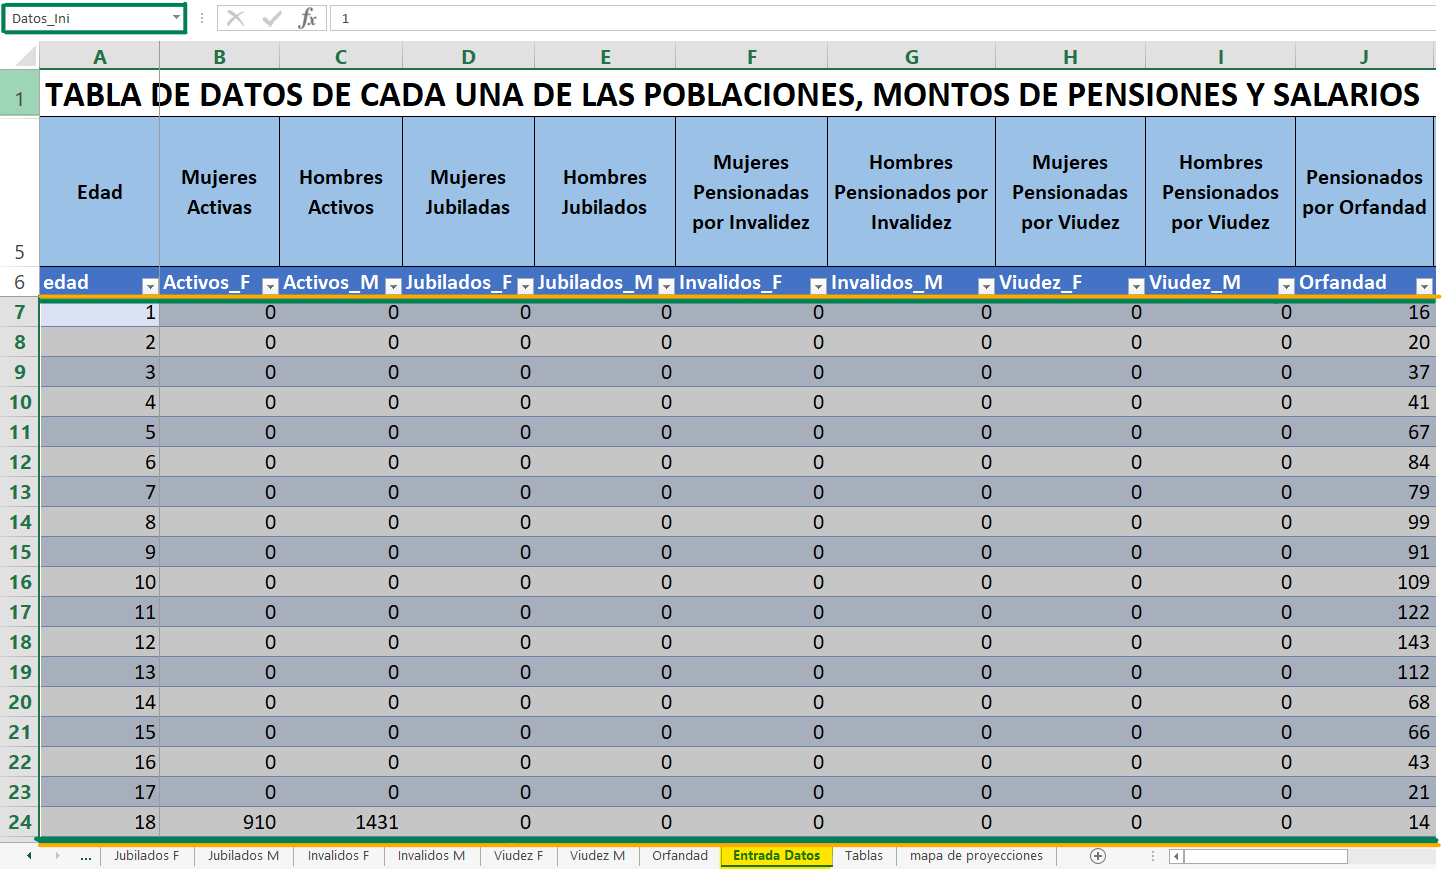
\includegraphics{images/F/Img1.png}

}

\caption{Hoja de entrada de datos}

\end{figure}

\hypertarget{tabla-para-escenario-de-revalorizaciuxf3n-de-pensiones}{%
\subsection{Tabla para Escenario de Revalorización de
Pensiones}\label{tabla-para-escenario-de-revalorizaciuxf3n-de-pensiones}}

A la información comprendida en esta tabla se le ha llamado
\emph{``Tpenrevalora''}. En esta sección se efectúan los cálculos para
mantener el poder adquisitivo de las pensiones a lo largo del tiempo de
otorgamiento del beneficio, tomando como parámetro de esta disminución
el efecto de alzas en el nivel de salarios, costo de la vida a partir de
la inflación y distribuyendo el incremento de conformidad a la escala
del beneficio adquirido, así como lo menciona el
\href{https://www.ilo.org/dyn/travail/docs/930/Reglamento\%20General\%20de\%20la\%20\%20Ley\%20del\%20IHSS.pdf}{Artículo
152} del Reglamento General de la Ley del Seguro Social.

\begin{itemize}
\tightlist
\item
  {[}\emph{Total de afiliados}{]} aquí se realiza la suma de las
  cantidades de pensionados Jubilados, Inválidos, Viudos y Orfandad por
  sexo, tomados de la tabla \emph{``Datos\_Ini''}
\end{itemize}

\[ 
Total\_af_{Y} =\sum_{x=1}^{110} Datos\_Ini[Y_x] 
\] Donde:

\(Total\_af_{Y}\) = cantidad total de afiliados por cada uno de los
tipos de beneficios \emph{Y}.\\
\(Y_x\) = cantidad de afiliados de Invalidez, Viudez, Orfandad y
Jubilados de edad \emph{x}.

\begin{itemize}
\item
  {[}\emph{Incremento por tipo de beneficio}{]} aquí se establece el
  nuevo monto para cada una de las pensiones de jubilados, inválidos,
  viudez y orfandad por sexo.
\item
  {[}\emph{Tpenrevalora}{]} aquí se establecen los cálculos para la
  revalorización de las pensiones promedios de los jubilados, inválidos,
  viudos y orfandad tanto por edad como por sexo, ejemplo:
\end{itemize}

\begin{equation} 
Tpenrev =\frac{Jubilados\_F \times Pen\_Jub\_F + \frac{Jubilados\_F}{Total\_af_{Jub} \times Incre\_bef_{Jub}}}{Jubilados\_F}
  \label{eq:Tpenrevalora}
\end{equation}

Donde:

\(Jubilados\_F\) = cantidad total de jubilados a la edad \emph{x}.\\
\(Pen\_Jub\_F\) = pensión promedio de jubilados de edad \emph{x}.\\
\(Total\_af\_{Jub}\) = cantidad total de afiliados jubilados.\\
\(Incre\_bef\_{Jub}\) = incremento por cada tipo de beneficio.

La fórmula antes descrita nos establece el monto promedio con la
revalorización de las pensiones para mujeres jubiladas, siguiendo esa
misma analogía se determina la revalorización para el resto de grupos y
género.

\begin{figure}

{\centering 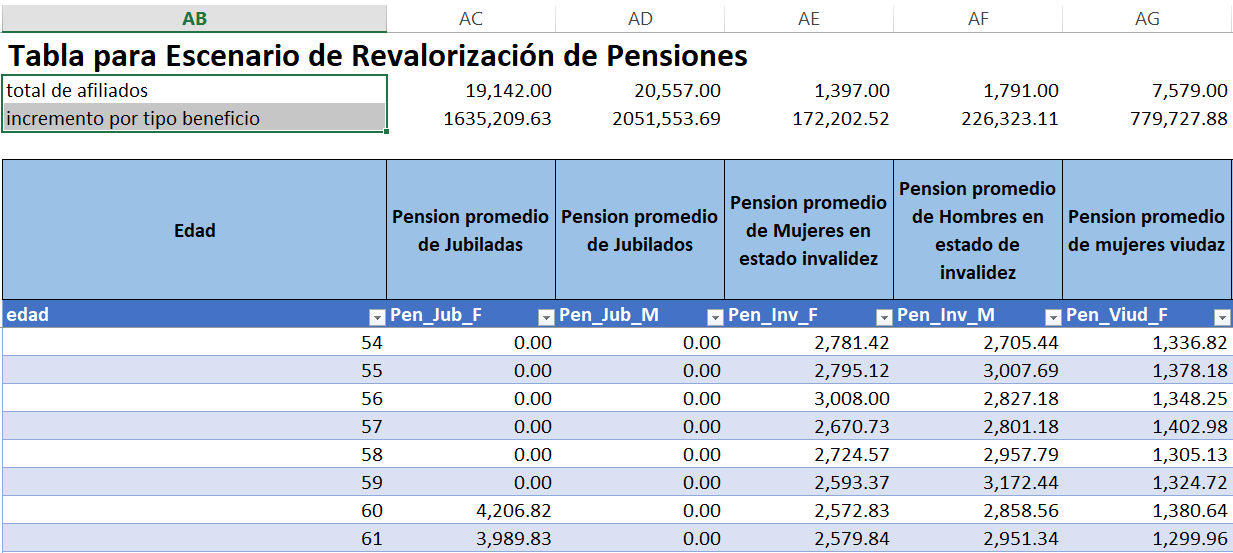
\includegraphics{images/F/Img2.png}

}

\caption{Tabla de Revalorización de pensiones}

\end{figure}

\bookmarksetup{startatroot}

\hypertarget{tablas-biomuxe9tricas}{%
\chapter{Tablas Biométricas}\label{tablas-biomuxe9tricas}}

\hypertarget{tablas}{%
\section{{[}Tablas{]}}\label{tablas}}

En esta sección nos encontramos con las distribuciones de probabilidad
según el estado del afiliado (Activo, Jubilado, Invalidez, Retiro,
Ingreso, Casado) por edad, a esta tabla se le ha llamado
\emph{``Tbiometrica''}, también incluimos dentro de esta, la sección de
decrementos múltiples y para este estudio en particular de 2022 se
tomaron en cuenta las probabilidades y tasas de mortalidad por efecto
del SARS-Cov-19 (Enfermedad por Coronavirus). Las probabilidades según
el estado del afiliado son extraídas conforme a lo indicado en la
Circular \emph{SPV No.~11/2017}, Memorando \emph{UNYS No.~1166-2017},
sobre el uso de Tablas Biométricas:

\begin{itemize}
\tightlist
\item
  Tabla de participantes activos
\item
  Tabla de jubilación estimada de los datos históricos del IHSS
\item
  Tabla de ingresos estimada de los datos históricos del IHSS
\item
  Mortalidad: 1980 Commissioners Standar Ordinary (CSO) -- Formerly
  Table K (F). Base: Age Nearest Birthday.
\item
  Invalidez: 1968-72 Total and Permanent Disability (50\% basis) Table
  -- Base: Age: Nearest Birthday
\item
  Rotación y despido: Tabla de mortalidad JONHIG
\item
  Tablas para pensionados
\item
  Mortalidad jubilados: Tabla de Mortalidad de Rentistas, Instituto de
  Seguros Sociales (TCMR ISS) 1980-1989
\item
  Mortalidad para inválidos: Tabla de mortalidad de inválidos,
  Superintendencia Bancaria de Colombia, Resolución 0585 de 1994
\item
  Tablas de probabilidad que un afiliado este casado corresponde al
  valor promedio del comportamiento histórico de los datos del IHSS.
\end{itemize}

\hypertarget{mortalidad}{%
\subsection{Mortalidad}\label{mortalidad}}

Estos bloques de información son las de mayor interés dentro del
análisis ya que nos permite estudiar los fallecimientos por sexo y edad.

\begin{itemize}
\tightlist
\item
  {[}\emph{qa\_X}{]} probabilidad de que un activo de género \emph{X}
  fallezca.
\item
  {[}\emph{qi\_X}{]} probabilidad de que un inválido de género \emph{X}
  fallezca.
\item
  {[}\emph{qj\_X}{]} probabilidad de que un jubilado de género \emph{X}
  fallezca.
\end{itemize}

\begin{figure}

{\centering 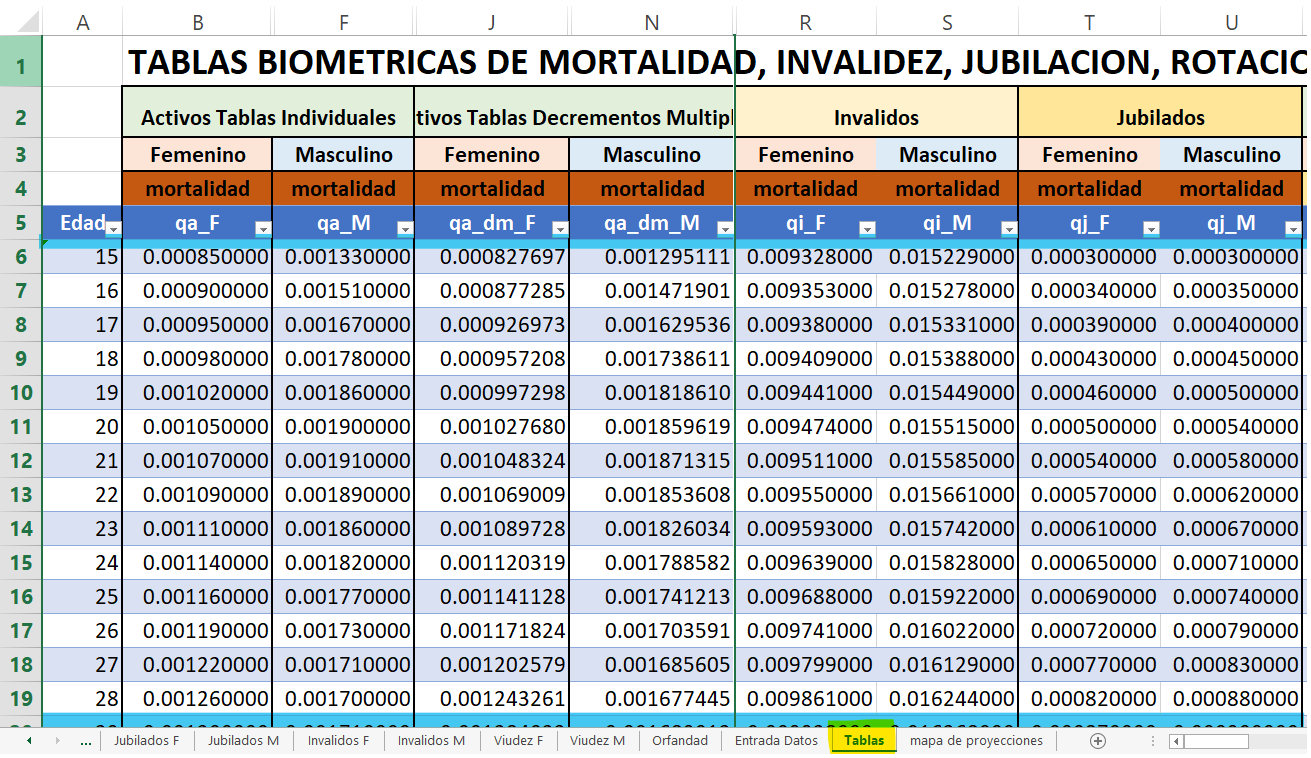
\includegraphics{images/F/Img3.png}

}

\caption{Probabilidades de mortalidad}

\end{figure}

\hypertarget{salida}{%
\subsection{Salida}\label{salida}}

En esta sección se incluyen las probabilidades de dejar de formar parte
de los cotizantes activos ya sea por retiro, jubilación o invalidez.

\begin{itemize}
\tightlist
\item
  {[}\emph{ra\_X}{]} probabilidad que un activo de género \emph{X} se
  retire.
\item
  {[}\emph{pja\_X}{]} probabilidad que un activo de género \emph{X} se
  jubile.
\item
  {[}\emph{ia\_X}{]} probabilidad que un activo de género \emph{X} se
  invalide.
\end{itemize}

\begin{figure}

{\centering 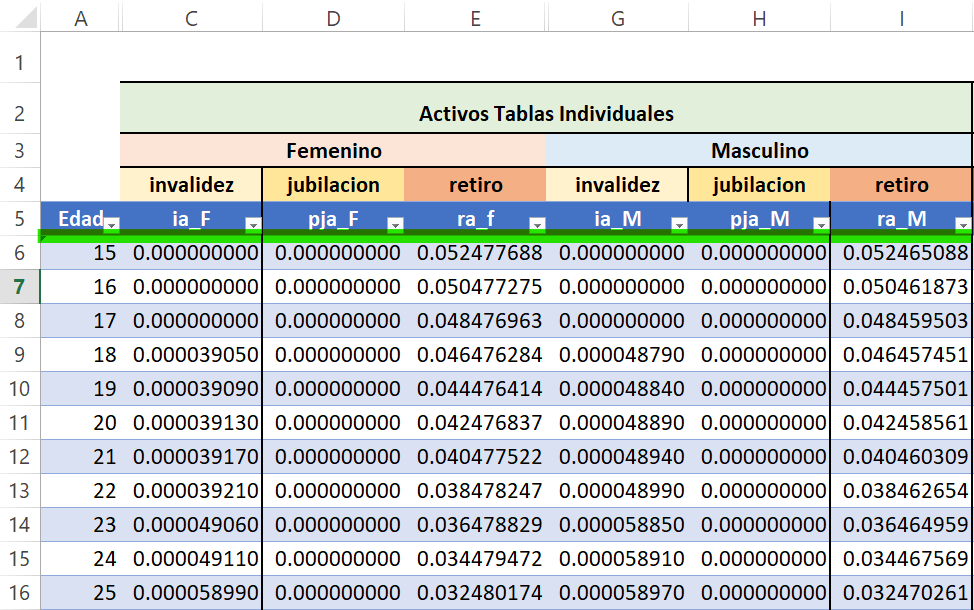
\includegraphics[width=5.65625in,height=\textheight]{images/F/Img4.png}

}

\caption{Probabilidades de salidas del sistema}

\end{figure}

En esta sección se toman en cuenta las probabilidades que tiene un
afiliado de ingresar al sistema

\begin{itemize}
\tightlist
\item
  {[}\emph{ping\_X}{]} probabilidad que un afiliado de género \emph{X}
  ingrese al sistema.
\end{itemize}

\begin{figure}

{\centering 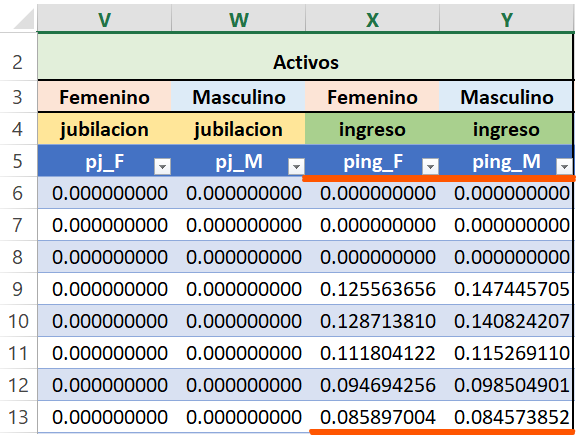
\includegraphics[width=4.15625in,height=\textheight]{images/F/Img5.png}

}

\caption{Probabilidades de ingreso al sistema}

\end{figure}

\hypertarget{estado-civil}{%
\subsection{Estado Civil}\label{estado-civil}}

Aquí se consideran las probabilidades que un afiliado este casado o
casada, esta distribución será la misma para ambos sexos y para todas
las edades.

\begin{itemize}
\tightlist
\item
  {[}\emph{pcas\_X}{]} probabilidad de que un afiliado de género
  \emph{X} este casado.
\end{itemize}

\begin{figure}

{\centering 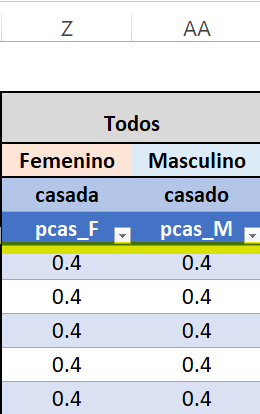
\includegraphics[width=1.85417in,height=\textheight]{images/F/Img6.png}

}

\caption{Probabilidades de estar casado}

\end{figure}

\hypertarget{decrementos-muxfaltiples}{%
\subsection{Decrementos Múltiples}\label{decrementos-muxfaltiples}}

Aquí se toman en cuenta las probabilidades de que un afiliado abandone
el sistema por una única causa (Muerte, Vejez, Invalides, Retiro), para
ello se hace uso de la fórmula 2.1 para estimar probabilidades de los
decrementos múltiples que se encuentra en (Nota Técnica de Proyección de
Flujos del Régimen del Seguro de Previsión Social, a diciembre 2020):

\begin{align} q_x^{(k)} &= q_x^{\prime(k)} \left( 1-\frac{\sum_{i=1,i\neq k}^{4}q_x^{\prime(i)}}{2} + \frac{q_x^{\prime(k+1)}\times q_x^{\prime(k+2)}+\left(q_x^{\prime(k+1)}+q_x^{\prime(k+2)}\right)\times q_x^{\prime(2+3)}}{3}\right.\nonumber  \\ &\qquad \left.\vphantom{\int_t} -\frac{\prod_{i=1,i\neq k}^{4}q_x^{\prime(i)}}{4} \right) \end{align}

Donde:

\(q_x^{(i)}\): probabilidad de salir del grupo por la causa \emph{i}
para una persona de edad \emph{x}.\\
\(q_x^{\prime(i)}\): probabilidad individual de salir de un grupo por la
causa \emph{i} para una persona de edad \emph{x}.\\
\(i\): causa de salida, \(i=1,2,3,4...\)

Nota: entiéndase la notación siguiente como \((i+x)=modulo(i+x,4)\)

{[}\emph{qa\_dm\_X}{]} probabilidades de decremento múltiple de que un
activo de género \emph{X} fallezca.\\
{[}\emph{ia\_dm\_X}{]} probabilidad de decremento múltiple de que un
activo de género \emph{X} se invalide.\\
{[}\emph{pja\_dm\_X}{]} probabilidad de decremento múltiple de que un
activo de género \emph{X} se jubile.\\
{[}\emph{ra\_dm\_F}{]} probabilidad de decremento múltiple de que un
activo de género \emph{X} se retire.

A continuación se muestra un ejemplo de decrementos múltiples para el
caso de la mortalidad para cotizantes activos de sexo femenino:

\[=[@[qa_F]]*(1-SUMA(Tbiometrica[@[ia_F]:[ra_f]])/2+\]
\[([@[ia_F]]*[@[pja_F]]+([@[ia_F]]+[@[pja_F]])*[@[ra_f]])/3\]
\[-PRODUCTO(Tbiometrica[@[ia_F]:[ra_f]])/4)]\]

\begin{figure}

{\centering 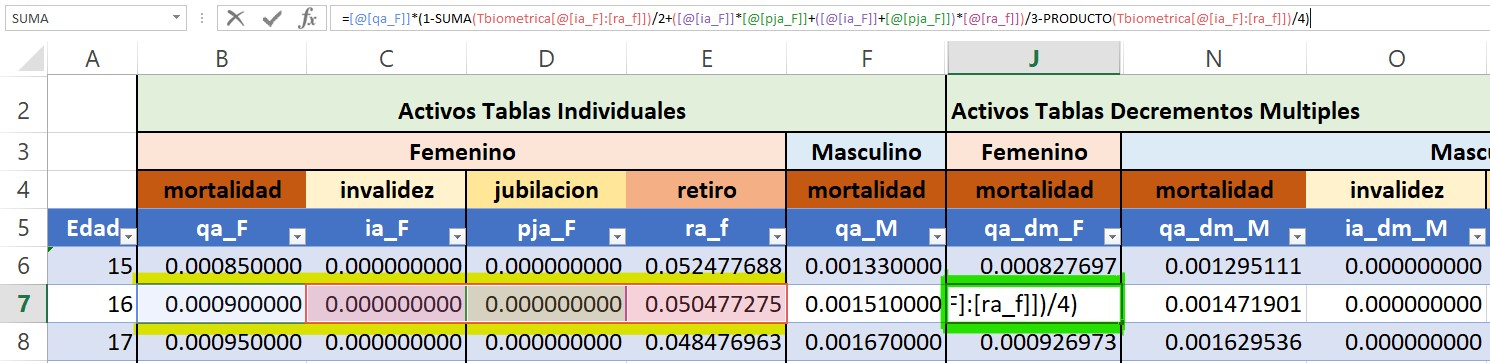
\includegraphics[width=6.53125in,height=\textheight]{images/F/Img7.jpg}

}

\caption{Ejemplo en tabla de decrementos multiples}

\end{figure}

\hypertarget{probabilidades-de-tener-hijos-de-cada-edad-hasta-los-18-auxf1os}{%
\subsection{Probabilidades de Tener Hijos de Cada Edad Hasta los 18
Años}\label{probabilidades-de-tener-hijos-de-cada-edad-hasta-los-18-auxf1os}}

\begin{itemize}
\tightlist
\item
  \textbf{Afiliados Activos}: esta tabla contiene las probabilidades de
  tener hijos de las distintas edades para afiliados activos de edad
  \emph{x}, a esta tabla se le ha llamado \emph{``Tphijos\_A''}
\end{itemize}

\begin{figure}

{\centering 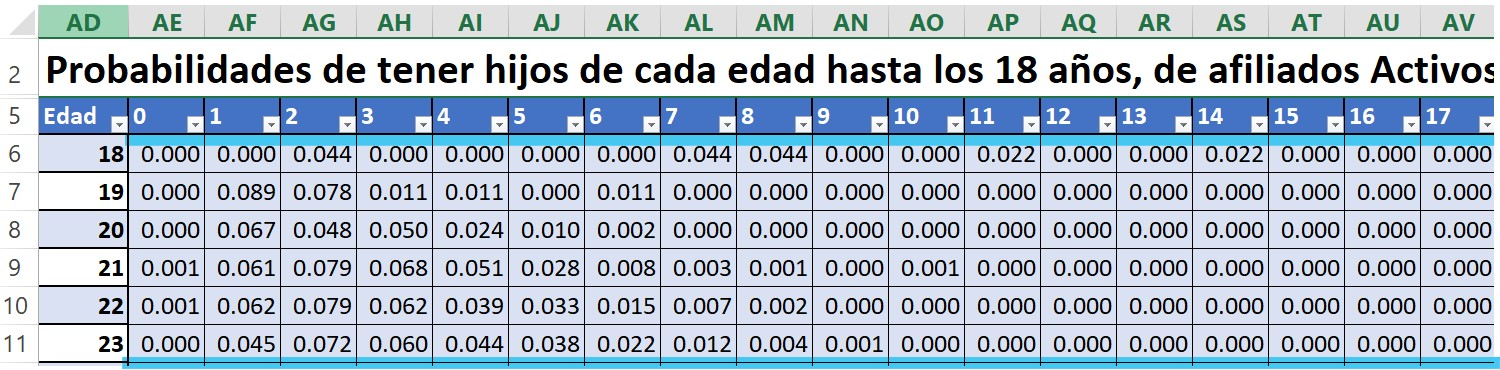
\includegraphics[width=6.5625in,height=\textheight]{images/F/Img8.jpg}

}

\caption{Probabilidad de que un activo tenga hijos}

\end{figure}

\begin{itemize}
\item
  \textbf{Jubilados}: esta tabla contiene las probabilidades de tener
  hijos de las distintas edades por edad de jubilados, a esta tabla se
  le ha llamado \emph{``Tphijos\_J''}.

  \begin{figure}

  {\centering 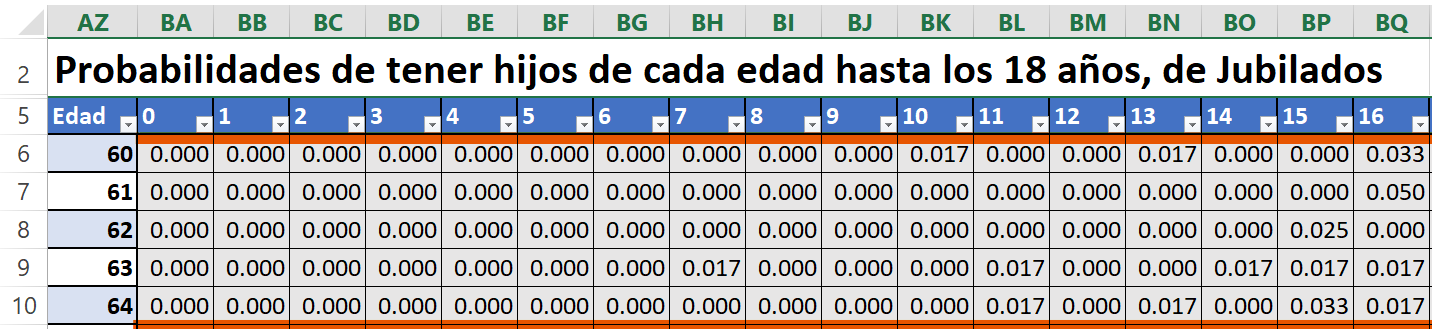
\includegraphics[width=7.29167in,height=\textheight]{images/F/Img9.png}

  }

  \caption{Probabilidad que un jubilado tenga hijos}

  \end{figure}
\item
  \textbf{Invalidez}: esta tabla contiene las probabilidades de tener
  hijos de las distintas edades por edad de afiliados inválidos, a esta
  tabla se le ha llamado \emph{``Tphijos\_I''}.
\end{itemize}

\begin{figure}

{\centering 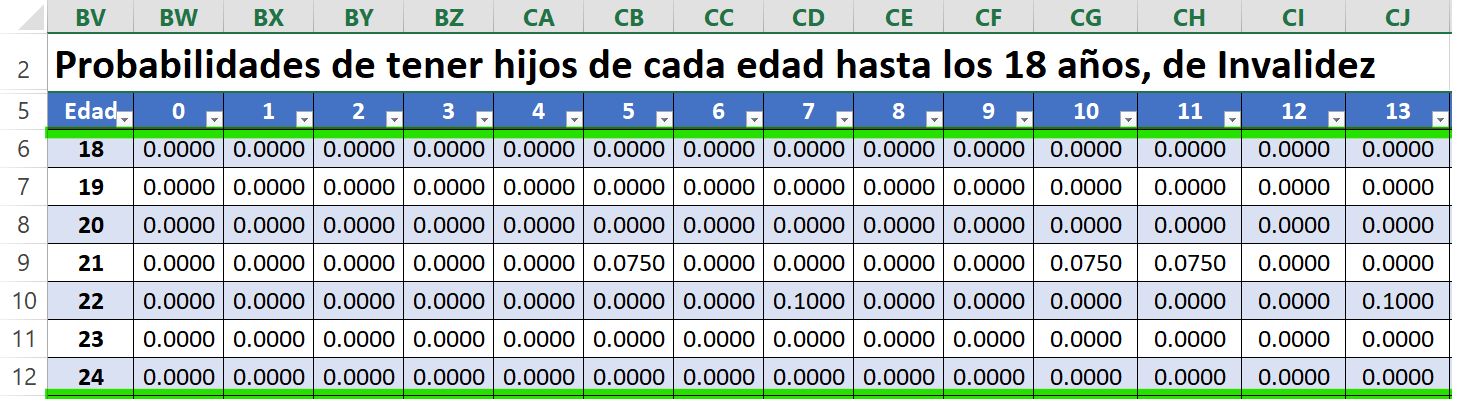
\includegraphics[width=6.5625in,height=\textheight]{images/F/Img10.png}

}

\caption{Probabilidad de que un invalido tenga hijos}

\end{figure}

\hypertarget{tasas-de-mortalidad-y-probabilidades-por-efecto-covid-19}{%
\subsection{Tasas de Mortalidad y Probabilidades por Efecto
COVID-19}\label{tasas-de-mortalidad-y-probabilidades-por-efecto-covid-19}}

Para el Estudio Actuarial con cifras a Diciembre de 2020 se consideraron
los efectos en las tasas de mortalidad y sus respectivas probabilidades
a causa de la pandemia por COVID-19. En la tabla de tasas de mortalidad
por COVID se incluyen valores como el rango de edad de las personas, el
número de fallecidos para cada uno de los rangos de edad, el número de
contagios, los contagios que se esperan alcanzar y las respectivas tasas
de mortalidad

\begin{itemize}
\tightlist
\item
  La columna \('DW'\) llamada {[}\emph{Contag-Expand}{]}, lo que realiza
  es un producto con cada fila de la columna \('DV'\) llamada
  {[}\emph{Contagios}{]} y el {[}\emph{factor\_exp}{]} cuyo valor
  constante es \emph{38}.
\end{itemize}

\[[DW_i={DV}_i \ast factor\_exp]\] Donde \emph{i} es la fila del archivo
en Excel.

\begin{itemize}
\tightlist
\item
  La columna \('DX'\) llamada {[}\emph{tasas\_de\_mortalidad}{]} se
  determina realizando el cociente de cada uno de los valores de la
  columna \('DU'\) llamada {[}\emph{fallecidos}{]} y
  {[}\emph{Contg\_Expand}{]}.
\end{itemize}

\[[DX_i={DU}_i/{DW}_i]\]

\begin{itemize}
\tightlist
\item
  La columna \('DY'\) llamada {[}\emph{suavizados}{]} se estima
  realizando un promedio del valor anterior y el siguiente de la
  {[}\emph{tasas\_de\_mortalidad}{]} a excepción del primer y último
  valor que se coloca el mismo valor.
\end{itemize}

\[DY_i=PROMEDIO({DX}_{i-1}:{DX}_{i+1})\]

\begin{itemize}
\tightlist
\item
  La columna \('DQ'\) llamada {[}\emph{q\_adicional}{]} es el factor
  adicional que se establecerá a las tablas de mortalidad recargadas por
  COVID-19, este se estima haciendo uso de la siguiente formula:
\end{itemize}

\[DQ_i=INDICE(\$DY\$6:\$DY\$27,COINCIDIR(Tcovid[@Edad]-1,\]
\[\$DT\$6:\$DT\$27,1)+1,1)*\$DQ\$4\]

**\emph{INDICE} esta se encarga de devolver el valor de una celda dentro
de la columna {[}\emph{suavizados}{]} en la posición de la fila y/o la
columna que ocupa dentro de ella.

**\emph{COINCIDIR} busca la edad de los afiliados en el intervalo de
celdas llamado {[}Hasta{]} y después devuelve la posición relativa de
dicho elemento en el rango.

\begin{figure}

{\centering 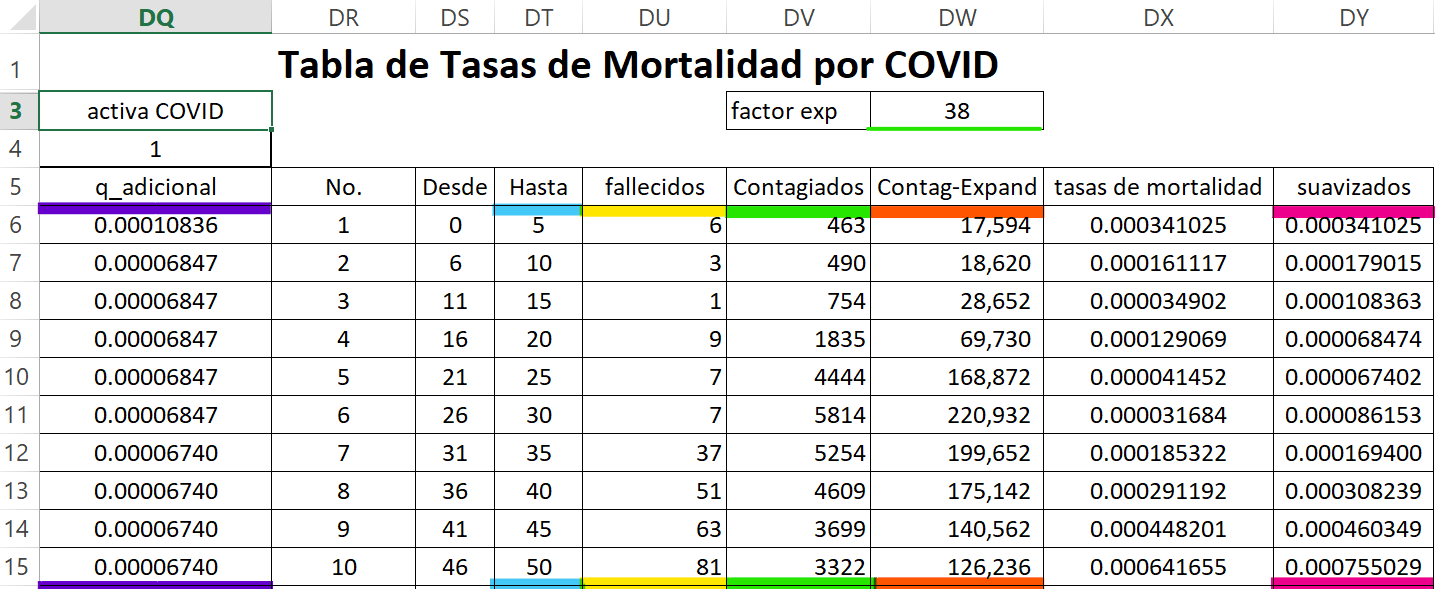
\includegraphics[width=7.52083in,height=\textheight]{images/F/Img11.png}

}

\caption{Tasas de mortalidad por COVID}

\end{figure}

\textbf{NOTA}: esta sección fue tomada para el análisis del Estudio
Actuarial con cifras a diciembre 2020 por la pandemia COVID-19, en otros
estudios estos valores no son tomados en cuenta.

A la tabla de probabilidades recargadas por COVID-19 se le ha llamado
\emph{``Tcovid''} y este valor resulta de la suma de las tablas
biométricas de mortalidad ({[}\emph{qa}{]}, {[}\emph{qi}{]} y
{[}\emph{qj}{]}) \emph{``Tbiometrica''} más el valor calculado en la
tabla de tasas de mortalidad por COVID-19 llamada
{[}\emph{q\_adicional}{]}.

\[=Tbiometrica[@[q]]+DQ_i]\]

\begin{figure}

{\centering 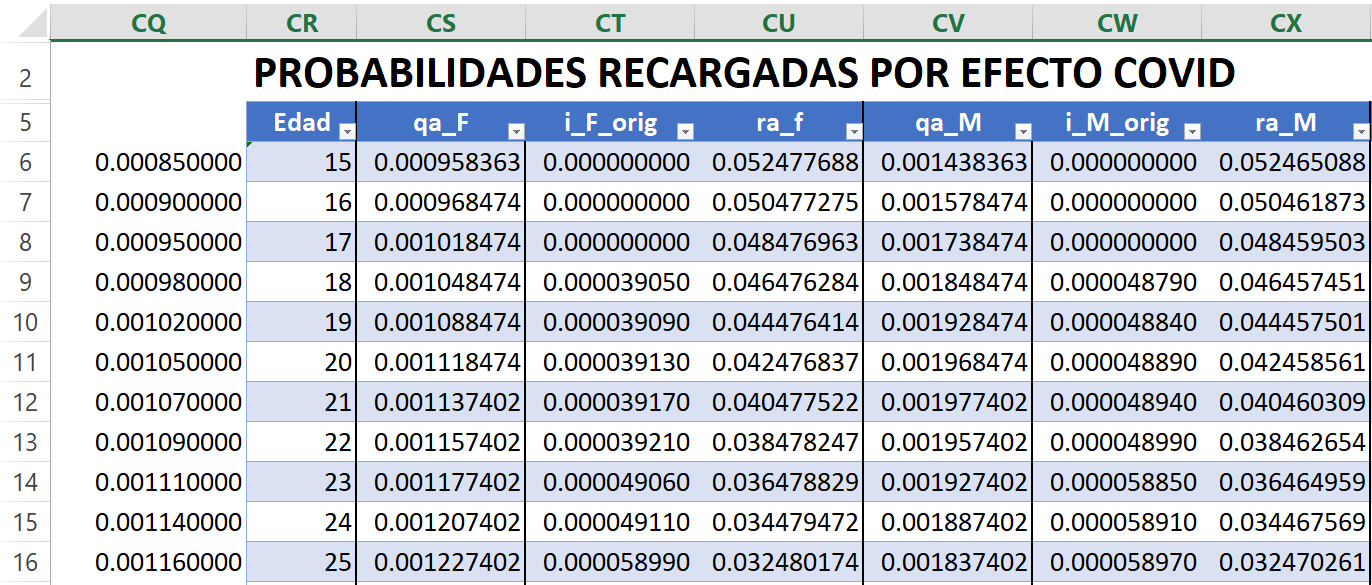
\includegraphics{images/F/Img12.png}

}

\caption{Probabilidades recargadas por efecto COVID}

\end{figure}

\bookmarksetup{startatroot}

\hypertarget{escenarios}{%
\chapter{Escenarios}\label{escenarios}}

\hypertarget{creaciuxf3n-de-escenarios-creaciuxf3n-escenarios}{%
\section{Creación de Escenarios {[}Creación
Escenarios{]}}\label{creaciuxf3n-de-escenarios-creaciuxf3n-escenarios}}

En esta sección se establece el conjunto de tablas que permiten modelar
y establecer parámetros que simulan distintos tópicos dentro del
régimen, estableciendo hipótesis o cambiando valores dependiendo del
tipo de escenario que se desee plantear. Estas tablas interactúan entre
sí con cada uno de los escenarios que se planteen y este se divide en
dos tablas: la tabla de escenarios y la tabla de valores de supuestos
por cada escenario.

\hypertarget{tabla-de-escenarios}{%
\subsection{Tabla de Escenarios}\label{tabla-de-escenarios}}

Los campos establecidos en esta tabla nos permiten agrupar los datos
posteriores en el tipo de escenario establecido, a esta tabla se le
llama \emph{``Tescenarios''}.

\begin{itemize}
\item
  {[}\emph{No.}{]} \textbf{Numero de Escenario}, se va generando
  mediante una secuencia y diferente en cada caso.
\item
  {[}\emph{Escenario}{]} \textbf{tipo de escenario}, escenario que se
  proyectará a esta tabla se le ha llamado \emph{``Lescenarios''}
\item
  {[}\emph{desc\_escena}{]} \textbf{Descripción de Escenario}, en este
  espacio agregamos una descripción relevante del tipo de escenario.
\item
  {[}\emph{prim\_pto\_c}{]} \textbf{Primer Punto Crítico}, año en el
  cual los ingresos corrientes que recibe el RSPS no son suficientes
  para cubrir los gastos y en este caso se recurre a los ingresos
  financieros.
\item
  {[}\emph{seg\_pto\_c}{]} \textbf{Segundo Punto Crítico}, este es el
  año en que el total de los ingresos que recibe el RSPS no son
  suficientes para cubrir el gasto total del régimen y es necesario
  tomar recursos del patrimonio.
\item
  {[}\emph{ter\_pto\_c}{]} \textbf{Tercer Punto Crítico}, año en que se
  ha consumido todo el patrimonio y ya no existen recursos para cubrir
  el déficit de ingresos para obtener el gasto total.
\item
  {[}\emph{num\_proy}{]} registra el Conteo de veces que esta un
  escenario en el almacén de proyecciones
\item
  Las celdas {[}\emph{Desde}{]} y {[}\emph{Hasta}{]} aquí establece el
  valor mínimo y máximo del número de escenarios que se han creado, esto
  servirá posteriormente para crear la proyección.
\item
  {[}\emph{Agregar\_Escenario}{]} este botón nos permite iniciar el
  proceso de proyección de flujos.
\end{itemize}

\begin{figure}

{\centering 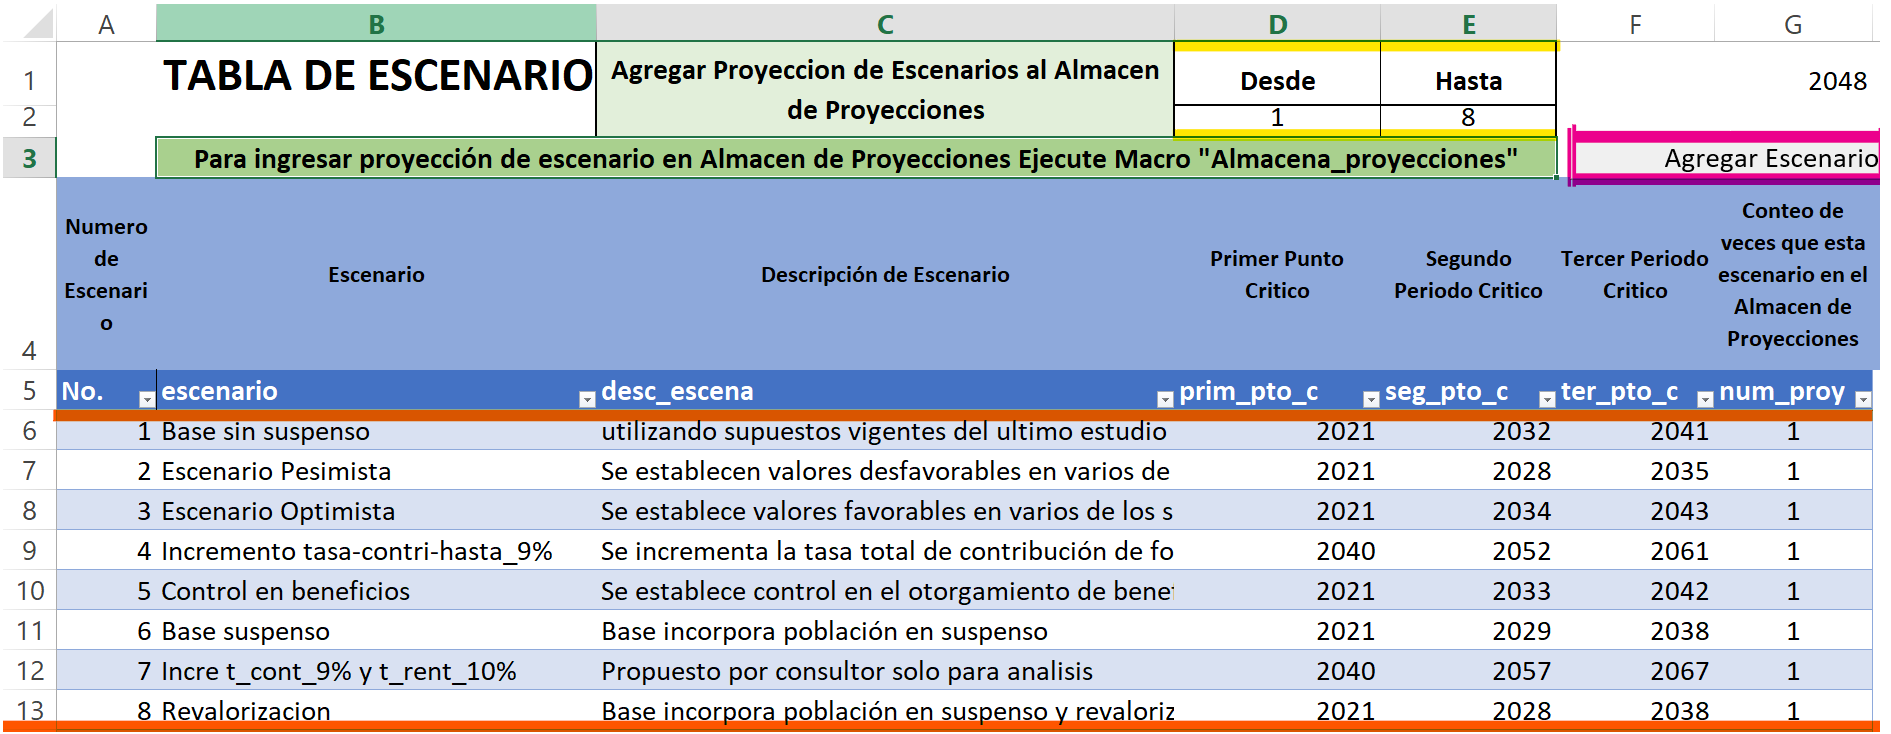
\includegraphics{images/F/Img13.png}

}

\caption{Tabla de creación de escenarios}

\end{figure}

\hypertarget{tabla-de-valores-supuestos-para-cada-escenario}{%
\subsection{Tabla de Valores Supuestos Para Cada
Escenario}\label{tabla-de-valores-supuestos-para-cada-escenario}}

En cada uno de los campos de esta sección se incluyen una gran variedad
de parámetros, se le ha llamado a esta tabla ``Tesena\_supues'' estos
valores van a depender de la información de diversas fuentes como ser
datos estadísticos y en su mayoría de la Ley del Seguro Social y sus
Reglamentos. Estos valores a su vez van a cambiar con el tipo de
escenario y supuesto que se establezca, eso lo veremos a detalle a
continuación.

\textbf{Escenarios que se establecieron}:

\begin{itemize}
\item
  Base (Con suspenso y sin suspenso)
\item
  Pesimista
\item
  Optimista
\item
  Incremento de la tasa de contribución
\item
  Control de beneficios
\item
  Incremento de la tasa total de contribución y la de rendimiento
  efectiva
\item
  Revalorización de pensiones.
\end{itemize}

Los escenarios antes mencionados son definidos para este estudio en
particular pero estos pueden variar considerando otros factores ya sea
por reformas de ley, comportamiento de los datos, por decisión de los
miembros del Comité de Asuntos Actuariales entre otros, es por ello que
esta sección es flexible a cambios.

\begin{itemize}
\item
  {[}\emph{act\_pob\_abierta}{]} \textbf{Proyección de población}, esta
  puede ser abierta y se establece el valor de 1 o cerrada y se define
  dicho valor como 0. (Para este estudio se tomarón en todos los
  escenarios como población abierta)
\item
  {[}\emph{por\_crece\_pob}{]} \textbf{Porcentaje de crecimiento de la
  población de afiliados}, es un dato de tipo demográfico y estadístico
  este índice se emplea con el fin de establecer cómo será el incremento
  de la población de afiliados del Regimen a lo largo de los años y en
  base a cada escenario planteado inicialmente.
\item
  {[}\emph{ttecnica\_real}{]} \textbf{Tasa Técnica Real}, es la Tasa de
  rentabilidad ajustada al efecto inflacionario, este valor depende de
  otros parámetros como ser la tasa de rendimiento efectiva
  {[}\(trend\_{efect}\){]} y la tasa de inflación
  {[}\(tinf\_{real}\){]}. Para ello se hace uso de la siguiente formula.
\end{itemize}

\begin{equation} 
ttecnica\_{real}=\frac{1+\ trend\_{efect}}{1+ tinf\_{real}}-1
 \label{eq:ttreal}
\end{equation}

\begin{itemize}
\item
  {[}\emph{trev\_pen}{]} \textbf{Tasa de revalorización de pensiones},
  este factor depende en su totalidad de la tasa de inflación, es por
  ello que colocamos el mismo valor en ambos campos.
\item
  {[}\emph{trev\_efect}{]} Tasa de rendimiento de las inversiones del
  fondo o la \textbf{Tasa de rendimiento efectiva} es un parámetro
  estadístico y nos permite ver el beneficio que se obtendrá por
  mantener dinero en un producto financiero o el rendimiento de una
  inversión a lo largo de los años proyectados y dependiendo del
  escenario que se plantee.
\item
  {[}\emph{tincre\_salarial}{]} \textbf{Tasa de incremento de los
  salarios sujetos de contribución}, este es un dato estadístico en el
  cual se analiza la opción a realizar un aumento en los salarios por
  contribuciones de un afiliado, este factor esta relacionado con la
  inflación
\item
  {[}\emph{ttot\_contri}{]} \textbf{Tasa total de contribución}, este
  parámetro es un elemento que se establece en el
  \href{https://honduras.eregulations.org/media/ley_del_seguro_social.pdf}{Articulo
  55-A} de la ley del Seguro Social el cual hace mención de que la tasa
  de cotización será de dos por ciento (\(2\%\)) para el empleador y del
  uno por ciento (\(1\%\)) para el trabajador afiliado, teniendo una
  tasa total de tres por ciento (\(3\%\)).
\item
  {[}\emph{por\_ga}{]} \textbf{Porcentaje de gastos administrativos} en
  relación al ingreso por contribuciones, este es un parámetro
  estadístico el cual representa el ajuste a todo lo relacionado con los
  egresos necesarios para el funcionamiento optimo del regimen. se
  mantiene en un ocho por ciento (\(8\%\)) en la mayor parte de los
  escenarios, excepto en aquel escenario que se busca un incremento en
  la tasa de contribución, ya que este parámetro es inversamente
  proporcional al porcentaje de gastos. Esta dado por la siguiente
  formula:
\end{itemize}

\begin{equation} 
por\_{ga}=\frac{0.03\times 0.08}{ttot\_{contri}}
 \label{eq:porga}
\end{equation}

\begin{itemize}
\item
  {[}\emph{num\_contri}{]} \textbf{Numero de contribuciones al año},
  según el reglamento del IHSS es de 12 contribuciones por año.
\item
  {[}\emph{por\_salud}{]} \textbf{Porcentaje Aporte Salud} para
  pensionados por Invalidez y vejez, este es un factor que se establece
  en el
  \href{https://www.ilo.org/dyn/travail/docs/930/Reglamento\%20General\%20de\%20la\%20\%20Ley\%20del\%20IHSS.pdf}{Articulo
  112} del reglamento para la atención medica de los jubilados y
  pensionados el cual es de diez punto cinco por ciento (\(10.5\%\)).
\item
  {[}\emph{num\_pension}{]} \textbf{número de pensiones por año}, se
  establece un total de 14 pensiones.
\item
  {[}\emph{dif\_edad\_matri}{]} \textbf{Diferencia de edades entre
  hombres y mujeres casados}, este es un dato de tipo estadístico el
  cual se establece en 5 años.
\item
  {[}\emph{tremp\_viudez}{]} \textbf{Tasa remplazo pensiones viudez}, es
  un beneficio establecido en el
  \href{https://www.ilo.org/dyn/travail/docs/930/Reglamento\%20General\%20de\%20la\%20\%20Ley\%20del\%20IHSS.pdf}{Artículo
  124} del Reglamento General de la ley del Seguro Social el cual se
  establece en \(40\%\)
\item
  {[}\emph{tremp\_orfa}{]} \textbf{Porcentaje de transferencia de
  pensión a cada huérfano}. Este beneficio se establece en el
  \href{https://www.ilo.org/dyn/travail/docs/930/Reglamento\%20General\%20de\%20la\%20\%20Ley\%20del\%20IHSS.pdf}{Artículo
  127} del reglamento del IHSS, el cual se establece en \(20\%\).
\item
  {[}\emph{tremp\_ascend}{]} \textbf{Tasa remplazo pensiones por
  ascendencia}, este beneficio se establece en el
  \href{https://www.ilo.org/dyn/travail/docs/930/Reglamento\%20General\%20de\%20la\%20\%20Ley\%20del\%20IHSS.pdf}{Artículo
  130} del Reglamento General de la ley del Seguro Social, el cual se
  establece en \(20\%\).
\item
  {[}\emph{tmin\_jubila}{]}Tiempo mínimo de cotización para jubilarse el
  cual corresponde a 15 años.
\item
  {[}\emph{ej\_min}{]} \textbf{Edad Mínima de Jubilación}, estos valores
  están establecidos en el
  \href{https://www.ilo.org/dyn/travail/docs/930/Reglamento\%20General\%20de\%20la\%20\%20Ley\%20del\%20IHSS.pdf}{Artículo
  116} del Reglamento General de la ley del Seguro Social los cuales se
  establecen como 60 años para mujeres y 65 para Hombres.
\item
  {[}\emph{por\_min\_jubila}{]} \textbf{Porcentaje mínimo de
  transferencia} de pensión a los sobrevivientes. Es un dato establecido
  en el
  \href{https://www.ilo.org/dyn/travail/docs/930/Reglamento\%20General\%20de\%20la\%20\%20Ley\%20del\%20IHSS.pdf}{Artículo
  117} del Reglamento General de la ley del Seguro Social, el cual se
  establece como valor mínimo el \(50\%\).
\item
  {[}\emph{por\_max\_jubila}{]} \textbf{Porcentaje máximo de
  transferencia} de pensión a los sobrevivientes. Es un dato establecido
  en el
  \href{https://www.ilo.org/dyn/travail/docs/930/Reglamento\%20General\%20de\%20la\%20\%20Ley\%20del\%20IHSS.pdf}{Artículo
  117} del Reglamento General de la ley del Seguro Social, el cual se
  establece como valor mínimo el \(80\%\).
\item
  {[}\emph{cred\_jubila}{]} \textbf{Porcentaje de Crédito unitario
  anual} para calcular tasa remplazo jubilación se establece en el
  \href{https://www.ilo.org/dyn/travail/docs/930/Reglamento\%20General\%20de\%20la\%20\%20Ley\%20del\%20IHSS.pdf}{Artículo
  111} del Reglamento General de la ley del Seguro Social.
\item
  {[}\emph{tprom\_jubila}{]} \textbf{Tiempo Promedio cotizado para
  jubilación} es un dato de tipo estadístico el cual se establece en 25.
\item
  {[}\emph{tprom\_remp\_jubila}{]} \textbf{Tasa de remplazo promedio de
  jubilación}, este es un factor que resulta de la aplicación de la
  siguiente formula:
\end{itemize}

\begin{equation} 
tprom\_remp\_jubila = \left ( tprom\_jubila - tmin\_jubila \right ) \times cred\_jubila + por\_min\_jubila
 \label{eq:tpromjubila}
\end{equation}

\begin{itemize}
\item
  {[}\emph{sa\_af\_inicio}{]} \textbf{Salario de referencia para otorgar
  beneficio de ayuda por sepelio}, este dato se establece en el
  \href{https://www.ilo.org/dyn/travail/docs/930/Reglamento\%20General\%20de\%20la\%20\%20Ley\%20del\%20IHSS.pdf}{Artículo
  57} del Reglamento General de la ley del Seguro Social. Para ello
  tomamos el valor más bajo de
  \href{https://www.ccichonduras.org/spanish/comunicados/2021/Junio/TABLA\%20AJUSTE\%20SALARIO\%20MINIMO.pdf}{(Tabla
  de Salario Mínimo Año 2021)}
\item
  {[}\emph{tcrece\_afunebre}{]} \textbf{Tasa de incremento del salario
  de referencia para otorgar beneficio de ayuda por sepelio}, este es un
  beneficio de tipo estadístico el cual representa el porcentaje de
  aumento que se le aplicara a lo largo de los años proyectados a la
  suma única de dinero que es pagada por concepto de ayuda con los
  gastos funerarios de un afiliado.
\item
  {[}\emph{activar\_susp}{]} \textbf{Activar afiliados en suspenso},
  para ello aplicamos el valar de uno (1) para activar la población en
  suspenso y cero (0) para desactivarlo.
\item
  {[}\emph{fact\_rec\_ga}{]} \textbf{Recargo por Gasto Administrativo},
  es un dato de tipo estadístico en el cual colocamos el valor de 1 para
  dejar el escenario sin recargo y mayor que uno en caso contrario.
\item
  {[}\emph{jub\_obli\_ehombre}{]} y {[}\emph{jub\_obli\_emujer}{]}
  \textbf{Edad de jubilación obligatoria} para hombres y mujeres, en
  este caso asignamos el valor de 110 años para desactivar la jubilación
  obligatoria.
\item
  {[}\emph{tinf\_real}{]} \textbf{Tasa de inflación}, es un dato
  económico en el cual se toman en cuenta diferentes efectos en cuanto a
  la política monetaria, en la mayoría de los escenarios es un valor que
  va cambiando con los años, a excepción de los escenarios Optimista en
  el cual se mantiene en su porcentaje más bajo y Pesimista se establece
  el más alto, esto para todos los años posteriores.
\item
  {[}\emph{act\_reval}{]} \textbf{activar revalorización}, para que el
  escenario a considerar realice una revalorización aplicamos 1, y si no
  queremos que revalorice colocamos 0. En todos los escenarios no se
  realiza revalorización a excepción del escenario que revaloriza las
  pensiones.
\end{itemize}

\bookmarksetup{startatroot}

\hypertarget{proyecciones-por-tipo-de-beneficio}{%
\chapter{Proyecciones por Tipo de
Beneficio}\label{proyecciones-por-tipo-de-beneficio}}

En esta sección se desarrollan las hojas que contemplan la proyección
del costo por tipo de beneficio y tipo de afiliado en base a la
información del año de estudio y con ello se proyecta a cien años, más
el comportamiento de las obligaciones que se deben cubrir con el fondo.
Se desglosan las seis hojas las cuales corresponden a afiliados activos,
afiliados en suspenso, jubilados, invalidez, viudez y orfandad por
género. En forma general estas hojas contienen especificaciones que
categorizan a estos grupos para analizarlos adecuadamente y estimar
proyección de nuevos ingresantes, variación en el salario o beneficios,
nuevas pensiones o decesos. Dichos resultados son concatenados en la
hoja de proyección de flujos donde se determinan como gastos por pago de
beneficios. A continuación veremos a detalle cada una de ellas y los
procesos que se implementan.

Tipos de beneficios:

\begin{itemize}
\tightlist
\item
  Activos
\item
  Suspenso
\item
  Jubilados
\item
  Inválidos
\item
  Viudez
\item
  Orfandad
\end{itemize}

\bookmarksetup{startatroot}

\hypertarget{activos}{%
\chapter{Activos}\label{activos}}

\hypertarget{activos-femeninos-activo-f}{%
\section{Activos femeninos {[}Activo
F{]}}\label{activos-femeninos-activo-f}}

En esta tabla se encuentra información detallada sobre la cantidad de
activos femeninos que se espera a lo largo de los años proyectados,
también información sobre los salarios, un resumen de todos estos datos
estimados, y otras proyecciones que son relevantes para el análisis, las
cuales describimos a continuación:

\hypertarget{proyecciuxf3n-de-las-personas}{%
\subsection{Proyección de las
personas}\label{proyecciuxf3n-de-las-personas}}

A esta tabla se le ha llamado \emph{``Tact\_F''} y aquí se estima la
cantidad de afiliados activos de género femenino, para determinar estos
datos se hacen uso de una serie de parámetros que se detallan a
continuación:
{[}\emph{qa\_dm}{]},{[}\emph{ia\_dm}{]},{[}\emph{ra\_dm}{]} y
{[}\emph{pja\_dm}{]} Probabilidades de fallecer, invalidez, retirarse y
jubilarse respectivamente. Estas son las probabilidades de que un
afiliado abandone el sistema, llamados decrementos múltiples las cuales
se encuentran en la hoja {[}\emph{Tablas}{]} en la matriz
\emph{``Tbiometrica''}

\begin{itemize}
\tightlist
\item
  {[}\emph{qtot}{]} Probabilidad total Salidas, este parámetro es la
  suma de todas las probabilidades antes descritas.
\item
  {[}\emph{pcas}{]} y {[}\emph{ping}{]} probabilidad de estar casada y
  probabilidad de ingresos al sistema.
\item
  {[}\emph{a1-a100}{]} son las cantidades de afiliados activos
  proyectadas que se realizan en el estudio, para este análisis se hace
  uso de la siguiente formula:
\end{itemize}

\begin{equation} 
{Can}_{x,j}=\ {Can}_{x-1,j-1}\times\left(1-{qtot}_{x-1}\right)+{ping}_x\times{Ingresos}_j
 \label{eq:canactivos}
\end{equation}

Donde:

\(Can_{x,j}\) = Cantidad de afiliados activos femeninos de edad x en el
año \emph{j}.\\
\(Can_{x-1,j-1}\) = Cantidad de afiliados activos femeninos de edad
\emph{x-1} en el año anterior.\\
\({qtot}_{x-1}\) = probabilidad total de salidas del sistema para un
afiliado de edad \emph{x-1}.\\
\({ping}_x\) = Probabilidad que un activo femenino de edad \emph{x}
ingrese al sistema.\\
\({Ingresos}_j\) = Cantidad de afiliados femeninos que ingresaron al
sistema en el año \emph{j}.

Lo antes descrito es una igualdad a la fórmula 3.3.9 Cantidad de
afiliados activos proyectada que se encuentra en (Nota Técnica de
Proyección de Flujos del Régimen del Seguro de Previsión Social, a
diciembre 2020)

\hypertarget{tabla-resumen}{%
\subsection{Tabla Resumen}\label{tabla-resumen}}

En esta sección se encuentra un resumen de información necesaria como lo
es el ingreso total de activos por años, las salidas de los mismos del
sistema, el porcentaje de crecimiento que se estima a lo largo de los
años entre otras, a continuación se describen a detalle cada una de
estas:

\begin{itemize}
\tightlist
\item
  {[}\emph{Total}{]} esta es la suma de todos los afiliados activos
  proyectados en el año \emph{j}.
\end{itemize}

\begin{equation}    
    Total_j=\sum_{x=18}^{110}{C{an}_{x,j}}
 \label{eq:totalactivos}
\end{equation}

\begin{itemize}
\tightlist
\item
  {[}\emph{Salidas}{]} representa la cantidad de afiliados activos que
  se esperan salgan del sistema en el año \emph{j}.
\end{itemize}

\begin{equation}    
Salidas_j=\sum_{x=18}^{109}{{qtot}_{x+1}\times{Can}_{x,j-1}}
 \label{eq:salidasact}
\end{equation}

Donde:

\({Can}_{x,j-1}\) = Cantidad de afiliados activos femeninos de edad
\emph{x} en el año anterior.\\
\({qtot}_{x+1}\) = probabilidad total de salidas del sistema para un
afiliado de edad \emph{x+1}.

\begin{itemize}
\tightlist
\item
  {[}\emph{Ingresos}{]} es la cantidad de nuevos ingresantes al sistema,
  si en la hoja llamada {[}\emph{Proyección supuestos}{]} la celda
  \emph{(act\_pob\_abierta) = 1} se realiza lo siguiente:
\end{itemize}

\begin{equation}
Ingresos_j=por\_{crece\_{pob}}\times{Total}_{j-1}+{Salidas}_j
\end{equation}

Donde:

\(por\_crece\_pob\) = porcentaje de crecimiento poblacional.\\
\({Total}_{j-1}\) = total de activos femeninos proyectados para el año
anterior.

\begin{itemize}
\tightlist
\item
  {[}\emph{verifica tasa crece}{]} representa la tasa de crecimiento
  poblacional proyectada relacionada con el año anterior y el presente,
  para ello se hace uso de la siguiente formula:
\end{itemize}

\begin{equation}
{vtc}_j=\frac{{Total}_j}{{Total}_{j-1}}-1
\end{equation}

Este parámetro se calcula como un valor agregado para comprobar que los
procedimientos realizados por Excel son verídicos, este dato es el mismo
al valor estadístico planteado al inicio del modelo al cual llamamos
porcentaje de crecimiento poblacional.

\begin{itemize}
\tightlist
\item
  {[}\emph{Fallecidos}{]} esta representa la suma total de la cantidad
  proyectada de fallecidos activos (para orfandad) llamada
  \emph{``Tfall\_AF''} ubicada en la misma tabla. Para ello hacemos uso
  de lo siguiente:
\end{itemize}

\begin{equation}
{Fallecidos}_j=\sum_{x=18}^{110}{Mue}_{x,j}
\end{equation}

\begin{figure}

{\centering 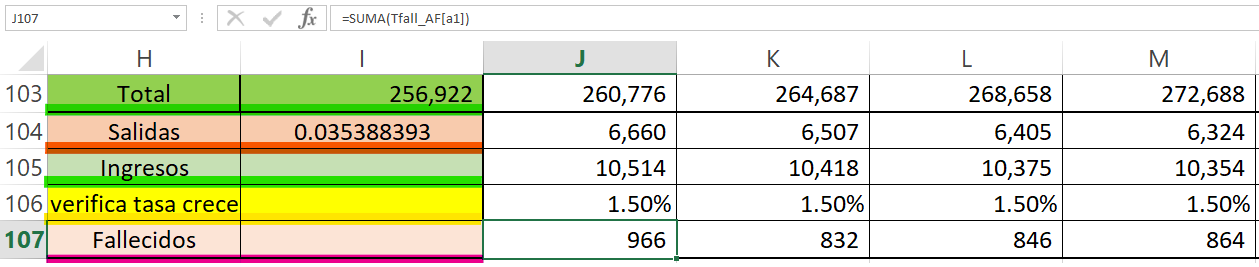
\includegraphics{images/F/Img14.png}

}

\caption{Tabla resumen para activos}

\end{figure}

\hypertarget{proyecciuxf3n-de-salarios}{%
\subsection{Proyección de salarios}\label{proyecciuxf3n-de-salarios}}

A esta tabla se le llamado \emph{``Tsalario\_F''}, para ello se hace uso
de la fórmula 3.3.10 Sueldo promedio de los afiliados activos
proyectado, que se encuentra en (Nota Técnica de Proyección de Flujos
del Régimen del Seguro de Previsión Social, a diciembre 2020)

\begin{equation}
{Sal\_act}_{x,j}= {Sal\_act}_{x,j-1}\times(1+{tincre\_sal}_j)
\end{equation}

Donde:

\({Sal\_act}_{x,j}\) = sueldo promedio de afiliados activos de edad
\emph{x} en el año \emph{j}.\\
\({Sal\_act}_{x,j-1}\) = sueldo promedio de afiliados activos de edad
\emph{x} en el año anterior.\\
\({tincre\_sal}_j\) = porcentaje de Incremento salarial en el año
\emph{j}.

\begin{figure}

{\centering 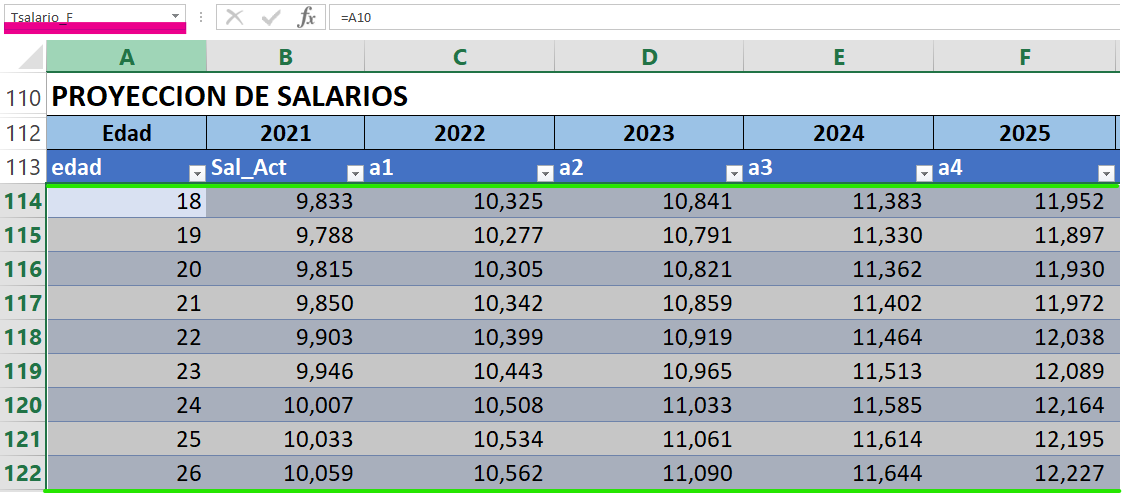
\includegraphics{images/F/Img15.png}

}

\caption{Proyección de salarios para activos}

\end{figure}

\hypertarget{resumen-de-proyecciuxf3n-de-datos}{%
\subsection{Resumen de Proyección de
datos}\label{resumen-de-proyecciuxf3n-de-datos}}

En esta tabla se realiza un resumen de las contribuciones y ayudas que
reciben los afiliados activos de género femenino, a esta tabla se le ha
llamado \emph{``Tresum\_AF''}. Para ello vemos a detalle cada uno de los
parámetros involucrados en dicha tabla

\begin{itemize}
\tightlist
\item
  {[}\emph{Contribuciones}{]} este dato representa la cantidad total de
  contribuciones por afiliados activos de género femenino, para dicho
  cálculo se hace uso de la fórmula 3.3.7 Total de contribución de
  afiliados activos, que se encuentra en (Nota Técnica de Proyección de
  Flujos del Régimen del Seguro de Previsión Social, a diciembre 2020)
\end{itemize}

\begin{equation}
{Contri}_j={num\_contri}_j\times{ttot\_contri}_j\ \times\sum{{Sal\_act}_{x,j}\times{Can}_{x,j}}
\end{equation}

Donde:

\({Contri}_j\) = total de contribución de afiliados activos en el año
\emph{j}.\\
\({ttot\_contri}_j\) = porcentaje de contribución que realizan los
afiliados activos.\\
\({num\_contri}_j\) = total de meses de contribución que realizan los
afiliados activos en el año.\\
\({Can}_{j,x}\) = cantidad de afiliados activos femeninos de edad
\emph{x} en el año \emph{j}.\\
\({Sal\_act}_{j,x}\) = sueldo promedio de los afiliados activos a la
edad \emph{x} en el año \emph{j}.

\begin{itemize}
\tightlist
\item
  {[}\emph{Ayuda Fúnebre}{]} este parámetro representa la cantidad
  monetaria que se le otorga a los familiares de los derecho-habientes
  jubilados, pensionados o fallecidos para gastos fúnebres, aquí se
  realiza un cálculo total por año proyectado, para ello se aplica la
  siguiente formula:
\end{itemize}

\begin{equation}
AFunebre_j=\ AFunbre_{j-1}\times(1+{tcrece\_afunebre}_j)
\end{equation}

Donde:

\(AFunbre_j\) = ayuda monetaria que se otorga en el año \emph{j}.\\
\(AFunbre_{j-1}\) = ayuda monetaria que se otorga en el año anterior.\\
\(tcrece\_afunebre\) = es la tasa de incremento del salario de
referencia para otorgar beneficio de ayuda por sepelio en el año
\emph{j}.

\begin{itemize}
\tightlist
\item
  {[}\emph{Tot.~Ben.~A.~F.}{]} Total de beneficios por ayuda fúnebre,
  este parámetro representa la cantidad total de beneficios que se
  conceden por ayuda fúnebre por toda la cantidad de fallecidos para el
  año proyectado
\end{itemize}

\begin{equation}
Tot.Ben.A.f_j=AFunebre_j\times{Fallecidos}_j
\end{equation}

\begin{figure}

{\centering 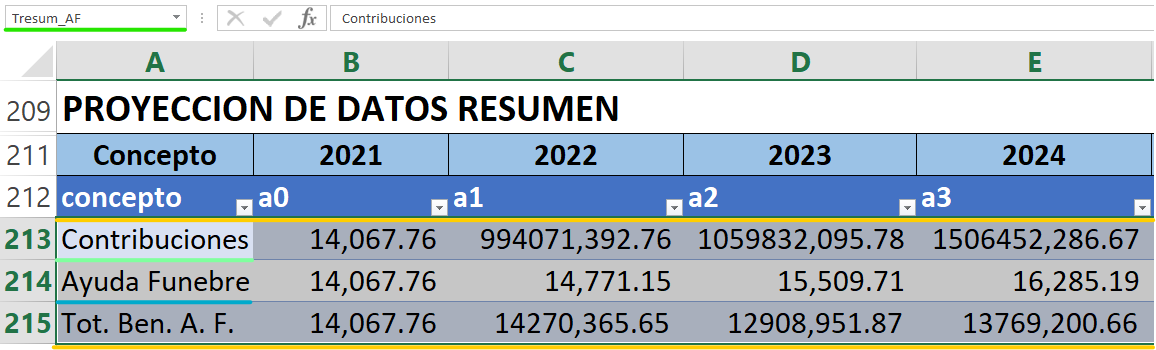
\includegraphics{images/F/Img16.png}

}

\caption{Tabla resumen de activos}

\end{figure}

\hypertarget{proyecciuxf3n-de-viudos}{%
\subsection{Proyección de viudos}\label{proyecciuxf3n-de-viudos}}

Este parámetro muestra la cantidad de viudos a la muerte de un activo
femenino, a esta tabla se le ha llamado \emph{``Tnviudez\_AFM''}, Para
estimar la proyección de viudos se toma en cuenta la probabilidad de
fallecer para un afiliado así como la probabilidad de estar casado.

\begin{equation}
CanV\_A_{x,j}={qa\_dm}_x\times pcas_x\times{Can}_{x-1+d,j-1}
\end{equation}

Donde:

\(CanV\_A_{x,j}\) = cantidad de viudos al fallecimiento de un activo de
edad \emph{x} en el año \emph{j}.\\
\({qa\_dm}_x\) = probabilidad de decremento múltiple de que un activo
fallezca a la edad \emph{x}.\\
\(pcas_x\) = probabilidad de que un afiliado este casado a la edad
\emph{x}.\\
\({Can}_{x-1+d,j-1}\) = cantidad de afiliados activos femeninos de edad
\emph{x-1} en el año anterior, \emph{d} representa la cantidad de año de
desfase de las edades entre hombre y mujeres tomando a \emph{d = -5} en
la tabla de féminas y \emph{d = 5} en masculino.

\begin{figure}

{\centering 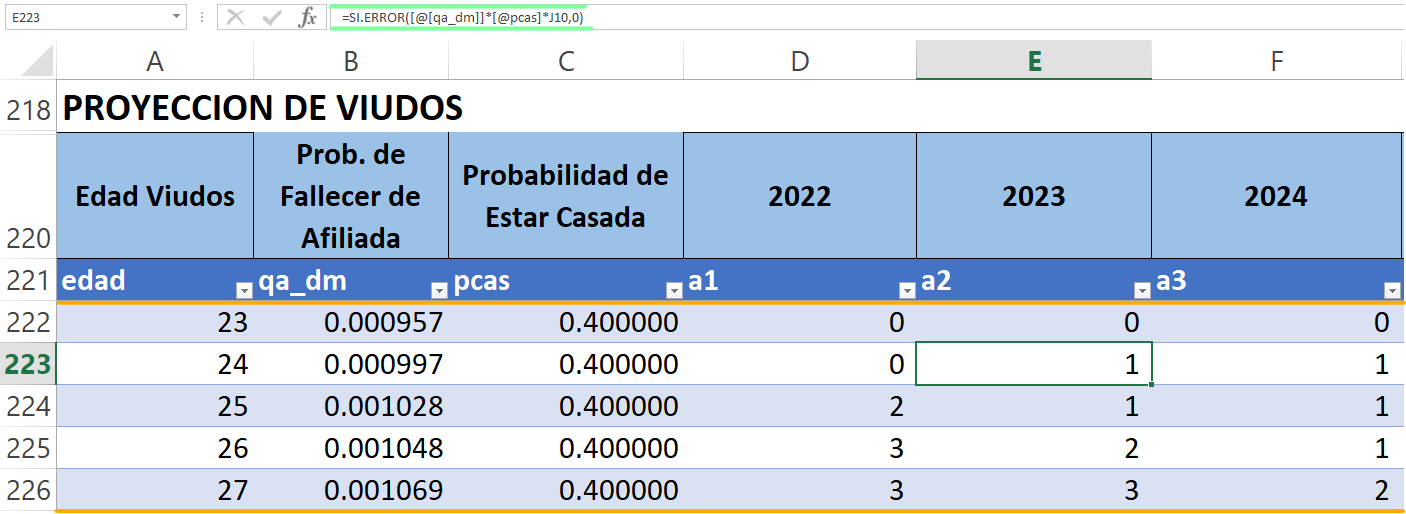
\includegraphics{images/F/Img17.png}

}

\caption{Proyección de viudos}

\end{figure}

\hypertarget{proyecciuxf3n-de-monto-calculado-de-pensiones-al-fallecimiento-de-activos-para-la-base-de-la-pensiuxf3n-por-viudez}{%
\subsection{Proyección de Monto Calculado de Pensiones al Fallecimiento
de Activos, Para la base de la pensión por
viudez}\label{proyecciuxf3n-de-monto-calculado-de-pensiones-al-fallecimiento-de-activos-para-la-base-de-la-pensiuxf3n-por-viudez}}

A esta tabla se le ha llamado \emph{``TMpenviud\_AFM''} y estos
parámetros se determinan haciendo uso de la siguiente formula, la cual
nos devuelve un porcentaje limitado por los valores \emph{0.5} y
\emph{0.8} los cuales representan los porcentajes mínimos y máximos de
transferencia de pensiones respectivamente formula llamada 1.3.2. Tasa
de Reemplazo a la edad de Jubilación la encontramos en (Valuación de
actualización Actuarial, pág. 220) y dicho valor es multiplicado por el
salario promedio de los activos.

\textbf{Tasa de Reemplazo a la Edad de Jubilación} \begin{equation}
TR=\ \left(t+x-ej-t_a\right)\times 1\%+50\%
\end{equation}

Donde:

\(TR\) = tasa de reemplazo a la edad de jubilación.\\
\(x\) = edad del afiliado.\\
\(ej\) = edad mínima de jubilación.\\
\(ta\) = tiempo de aportaciones a la edad \emph{x} en años.\\
\(t\) = tiempo total de aportaciones.

La ecuación antes establecida representa una igualdad a la fórmula
dentro de corchetes que se muestra a continuación que es la descrita en
el Excel.

\begin{equation}
tcot_j = {tprom\_{jub}}_j + x + d - {ej\_{min}}_j
  \label{eq:tcot}
\end{equation}

Donde:

\(tcot_j\) = tiempo cotizado de un afiliado para el año \emph{j}.\\
\({tprom\_{jub}}_j\) = tasa de reemplazo promedio de jubilación para el
año \emph{j}.\\
\(x+d\) = \emph{x} representa la edad del afiliado y \emph{d} la
diferencia de edades entre hombres y mujeres para este caso, en la tabla
femeninos \emph{d = -5} y en la tabla masculinos \emph{d = 0}\\
\({ej\_{min}}_j\) = edad mínima de jubilación para el año \emph{j}.

\begin{equation}
cred\_jubila_j = \frac{{tprom\_{remp\_{jub}}}_j-{por\_{min\_{jub}}}_j}{{tprom\_{jub}}_j-t{min\_{jub}}_j}
  \label{eq:credjub}
\end{equation}

Donde:

\(cred\_jubila_j\) = crédito unitario para el año \emph{j}.\\
\(t{min\_{jubila}}_j\) = tiempo mínimo de cotización para el año
\emph{j}.\\
\({tprom\_{remp\_{jub}}}_j\) = tasa de reemplazo promedio de jubilación
para el año \emph{j}.\\
\({por\_{min\_{jub}}}_j\) = porcentaje mínimo de transferencia de
pensión para el año \emph{j}.

Para determinar la proyección del monto de pensiones al fallecimiento de
un activo hacemos uso de las ecuaciones de crédito unitario y tiempo de
cotización, dada de la seguiente forma:

\begin{align} {Pen\_v}_{x,j} &= \left[ {por\_{min\_{jub}}}_j + \left( {\color{red}{tcot_j}} - \right. \right.\nonumber  \\ &\qquad \left. \left. tmin\_jub_j \right) \times {\color{gray}{cred\_jubila_j}}\right] \times Sal\_{act_{x+d,j}} \end{align}

Donde:

\({Pen\_v}_{x,j}\) = monto de pensiones al fallecimiento de un activo de
edad \emph{x} en el año \emph{j}.\\
\({Sal\_act}_{x+d,j}\) = sueldo promedio de afiliados activos de edad
\emph{x+d} en el año \emph{j}.

\begin{figure}

{\centering 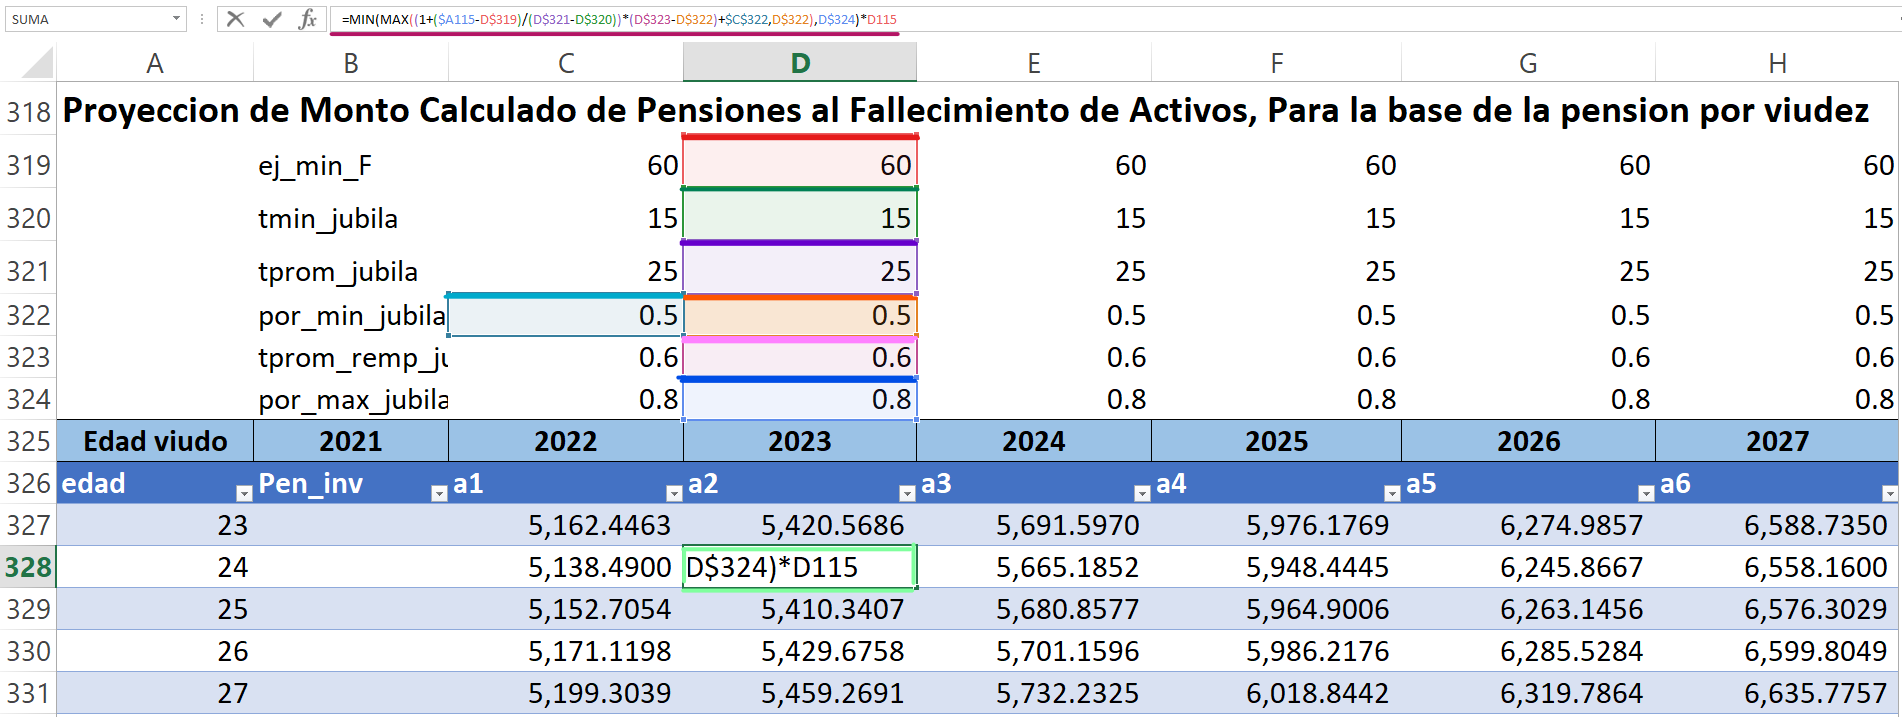
\includegraphics{images/F/Img18.png}

}

\caption{Proyección de pensiones al fallecimiento de activos}

\end{figure}

\hypertarget{proyecciuxf3n-del-producto-de-monto-pensiuxf3n-por-numero-de-pensiones-nuevas-de-viudez}{%
\subsection{Proyección Del Producto De Monto Pensión por Numero De
Pensiones Nuevas De
Viudez}\label{proyecciuxf3n-del-producto-de-monto-pensiuxf3n-por-numero-de-pensiones-nuevas-de-viudez}}

A esta tabla se le ha llamado \emph{``Tnew\_penxnum\_AFM''}, aquí se
establece el monto total de las pensiones para un viudo al fallecimiento
de su esposa activa, estos parámetros son el resultado de la
multiplicación del monto de pensión al fallecimiento de un activo de
edad \emph{x} en el año \emph{j} ubicados en la tabla
\emph{``TMpenviud\_AFM''} y el número de viudos proyectados de edad
\emph{x} en el año \emph{j}.

\begin{equation}
{TPen\_v}_{x,j}={Pen\_v}_{x,j}\times{CanV\_A}_{x,j}
\end{equation}

Donde:

\({TPen\_v}_{x,j}\) = monto Total de pensiones al fallecimiento de un
activo de edad \emph{x} en el año \emph{j}.\\
\({Pen\_v}_{x,j}\) = monto de pensiones al fallecimiento de un activo de
edad \emph{x} en el año \emph{j}.\\
\(Can{V\_A}_{x,j}\) = cantidad de viudos al fallecimiento de un activo
de edad \emph{x} en el año \emph{j}.

\begin{figure}

{\centering 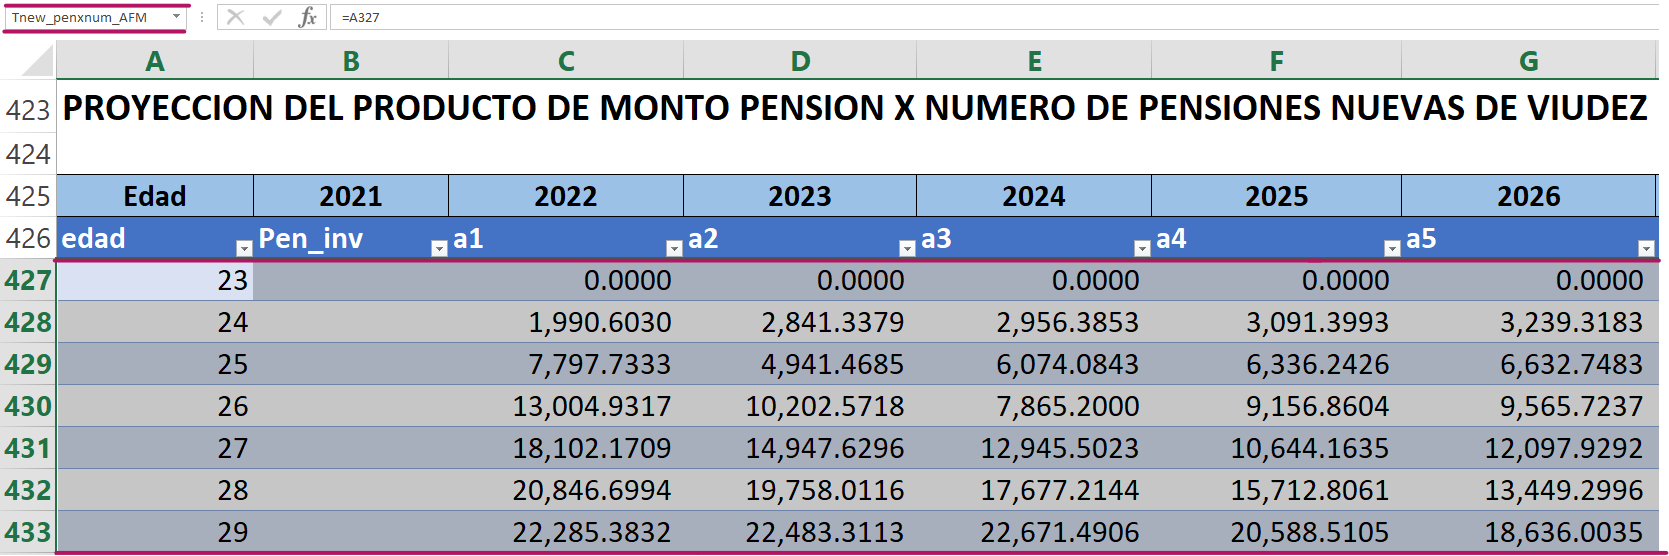
\includegraphics{images/F/Img19.png}

}

\caption{Proyección del monto de pensiones por número de pensiones
nuevas}

\end{figure}

\hypertarget{proyecciuxf3n-fallecidos-activos-principalmente-para-orfandad}{%
\subsection{Proyección Fallecidos Activos (Principalmente Para
Orfandad)}\label{proyecciuxf3n-fallecidos-activos-principalmente-para-orfandad}}

A esta tabla se le ha llamado \emph{``Tfall\_AF''}, aquí se establece la
cantidad de activos fallecidos de género femenino, dichos parámetros se
determinan haciendo el producto de la probabilidad de fallecer o salidas
por muerte {[}qa\_dm{]} de la sección de decrementos múltiples y la
cantidad de personas proyectadas de edad \emph{x-1} en el año anterior
\({Can}_{x-1,j-1}\) ubicados en la tabla \emph{``Tact\_F''}.

\begin{equation}
{Mue}_{x,j}={Can}_{x-1,j-1}\times{qa\_dm}_x
\end{equation}

Donde:

\(Mue_{x,j}\) = cantidad de afiliados activos que fallecen a la edad
\emph{x} en el año \emph{j}.\\
\(Can_{x-1,j-1}\) = cantidad de afiliados activos de edad \emph{x-1} en
el año anterior.\\
\({qa\_dm}_x\) = probabilidad de decremento múltiple de que un activo
fallezca a la edad \emph{x}.

\begin{figure}

{\centering 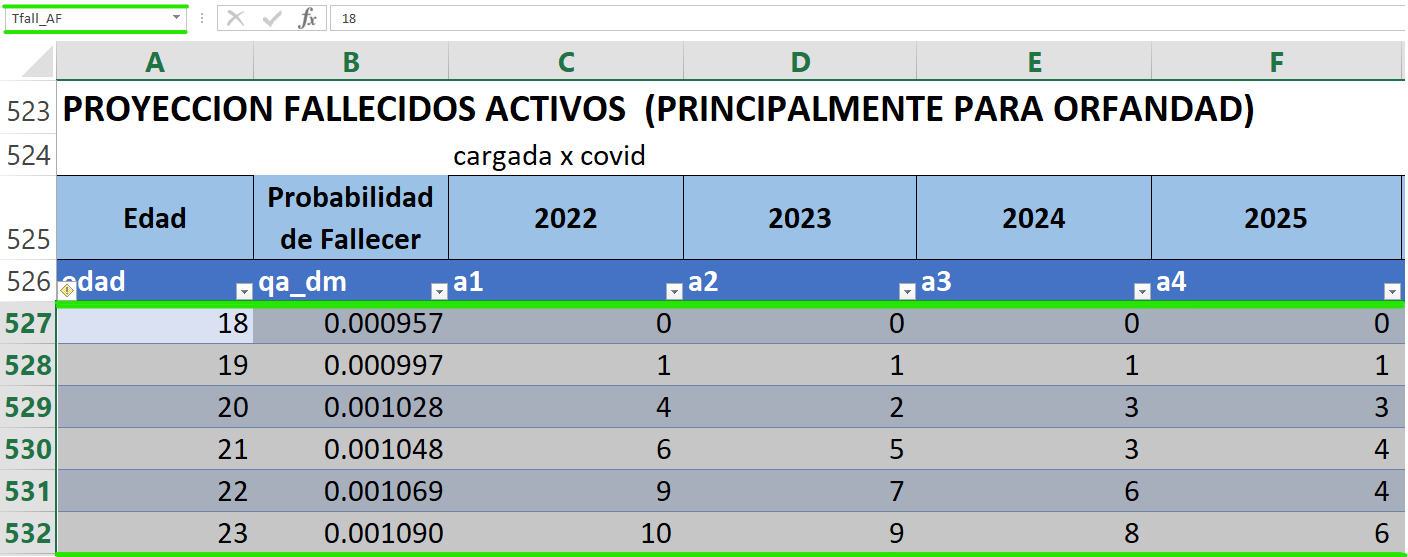
\includegraphics{images/F/Img20.png}

}

\caption{Proyección de activos fallecidos}

\end{figure}

\hypertarget{proyecciuxf3n-de-fallecidos-por-el-monto-de-pensiuxf3n}{%
\subsection{Proyección De Fallecidos Por El Monto De
Pensión}\label{proyecciuxf3n-de-fallecidos-por-el-monto-de-pensiuxf3n}}

A esta tabla se le ha llamado \emph{``Tpenfall\_AF''} Este parámetro
determina la cantidad de pensión total proyectada para todos los
fallecidos de edad \emph{x} en el año \emph{j} , este se obtiene
multiplicando la probabilidad de fallecer {[}qa\_dm{]} por el monto
calculado de pensiones al fallecimiento de activos de edad \emph{x} en
el año \emph{j} ubicados en la tabla \emph{``TMpenviud\_AFM''} y la
cantidad de activos proyectados para el año anterior
\({\ CantA}_{j-1,x-1+z}\) ubicado en la tabla \emph{``Tact\_F''}.

\begin{equation}
{TMue}_{x,j}={qa\_dm}_x\times{Pen\_v}_{x+5,j}\times{Can}_{x-1+d,j-1}
\end{equation}

Donde:

\({TMue}_{j,x}\) = cantidad total de montos de pensiones por
fallecimiento de activo de edad \emph{x} en el año \emph{j}.\\
\({qa_dm}_x\) = probabilidad de decremento múltiple de que un activo
fallezca a la edad \emph{x}.\\
\(Can_{j-1,x-1+z}\) = cantidad de afiliados activos proyectada a la edad
de \emph{x-1+d} años para el año anterior, \emph{d = 0} en caso femenino
y \emph{d = 5} en caso masculino.\\
\({Pen\_v}_{x,j}\) = monto de pensiones al fallecimiento de un activo de
edad \emph{x} en el año \emph{j}.

\begin{figure}

{\centering 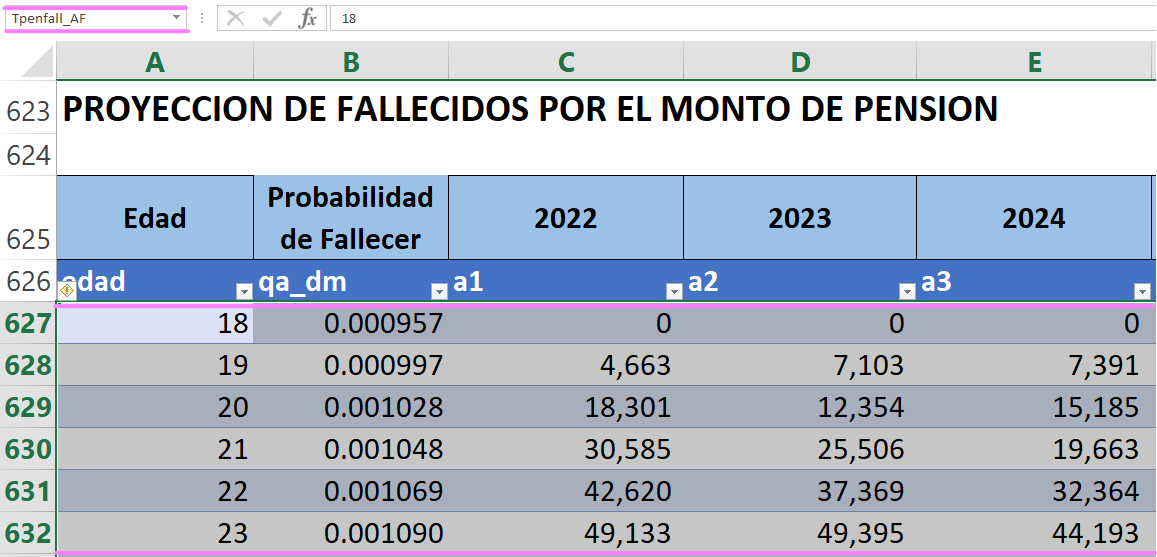
\includegraphics{images/F/Img21.png}

}

\caption{Proyección de fallecidos por el monto de pension}

\end{figure}

\textbf{NOTA}: Todos los parámetros y tablas antes descritas siguen el
mismo patrón y proceso para el caso masculino, habiendo ligeros cambios
en los nombres y variables siendo estos cambios por la inicial del
género (\emph{M}).

\bookmarksetup{startatroot}

\hypertarget{suspenso}{%
\chapter{Suspenso}\label{suspenso}}

\hypertarget{suspensos-femeninos-suspenso-f}{%
\section{Suspensos Femeninos {[}Suspenso
F{]}}\label{suspensos-femeninos-suspenso-f}}

En esta tabla se encuentra información detallada sobre la cantidad de
personas femeninas en suspenso que se espera a lo largo de los años
proyectados, también información sobre los salarios, un resumen de todos
estos datos estimados, y otras proyecciones que son relevantes para el
análisis, las cuales describimos a continuación.

\hypertarget{proyecciuxf3n-de-las-personas-1}{%
\subsection{Proyección de las
personas}\label{proyecciuxf3n-de-las-personas-1}}

A esta tabla se le ha llamado \emph{``Tsus\_F''} está contiene las
probabilidades de fallecer y jubilarse, así como los datos proyectados
de las personas en suspenso de edad \emph{x} a lo largo de los años
\emph{j}. Para el cálculo de estos parámetros se muestra la siguiente
formula:

\begin{equation}
Ca{nS}_{x,j}=Ca{nS}_{x-1,j-1}\times\left(1-{qa}_{x-1}-p{ja\_dm}_{x-1}\right)
\end{equation}

Donde:

\(Ca{nS}_{x,j}\) = cantidad de afiliados en suspenso de edad \emph{x} en
el año \emph{j}.\\
\({CanS}_{x-1,j-1}\) = cantidad de afiliados en suspenso de edad
\emph{x-1} en el año anterior.\\
\({qa}_x\) = probabilidad de que un activo fallezca a la edad
\emph{x}.\\
\(p{ja\_dm}_x\) = probabilidad de decremento múltiple de que un activo
se jubile a la edad \emph{x}.

\begin{figure}

{\centering 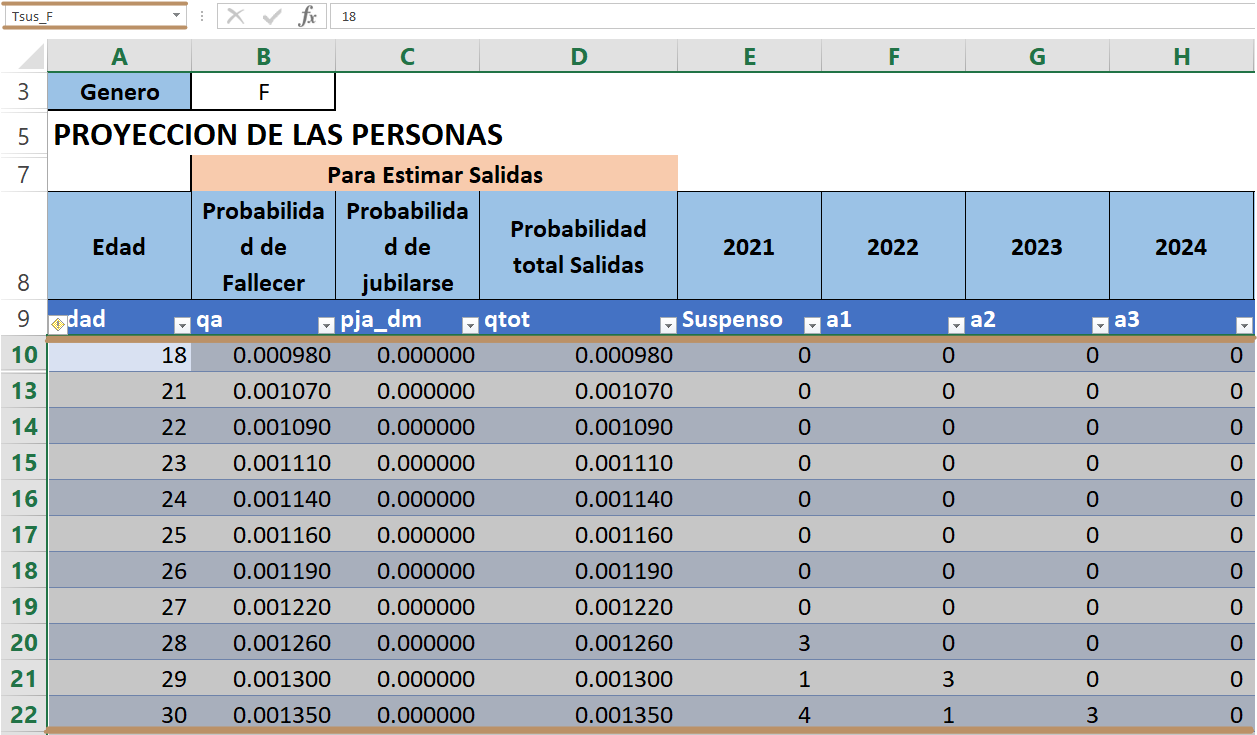
\includegraphics{images/F/Img22.png}

}

\caption{Cantidad de afiliados en suspenso}

\end{figure}

\hypertarget{proyecciuxf3n-de-salarios-1}{%
\subsection{Proyección De Salarios}\label{proyecciuxf3n-de-salarios-1}}

A esta tabla se le llamado \emph{``Tsal\_sus\_f''}, y contiene la
proyección de los salarios para un suspenso, para ello se hace uso de la
fórmula 4.3.4 Sueldo promedio de los afiliados en suspenso proyectado,
que se encuentra en (Nota Técnica de Proyección de Flujos del Régimen
del Seguro de Previsión Social, a diciembre 2020)

\begin{equation}
{Sal\_sus}_{x,j}=\ {Sal\_sus}_{x-1,j-1}\times(1+{tincre\_sal}_j)\ \end{equation}

Donde:

\({Sal\_sus}_{x,j}\) = salario promedio de los afiliados en suspenso de
edad \emph{x} en el año \emph{j}.\\
\({Sal\_sus}_{x-1,j-1}\) = salario promedio de los afiliados en suspenso
de edad \emph{x-1} en el año anterior.\\
\({tincre\_sal}_j\) = tasa de incremento salarial en el año \emph{j}.

\begin{figure}

{\centering 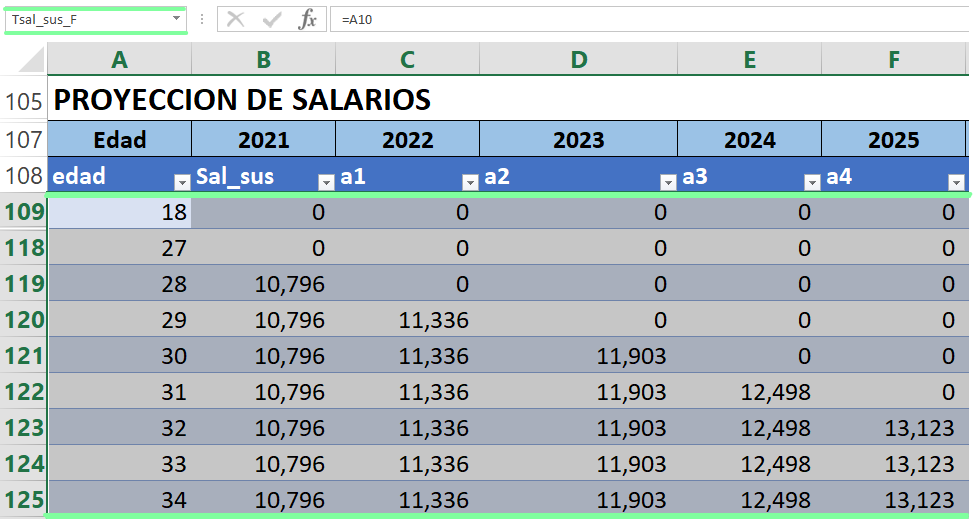
\includegraphics{images/F/Img23.png}

}

\caption{Proyección de salarios para personas en suspenso}

\end{figure}

\hypertarget{proyecciuxf3n-de-monto-calculado-de-pensiones-de-vejez-de-afiliados-en-suspenso}{%
\subsection{Proyección de Monto Calculado de Pensiones de vejez de
Afiliados en
Suspenso}\label{proyecciuxf3n-de-monto-calculado-de-pensiones-de-vejez-de-afiliados-en-suspenso}}

A esta tabla se le ha llamado \emph{``Tpenvej\_sus\_F''} y estos
parámetros se determinan haciendo uso de la siguiente formula, la cual
nos devuelve un porcentaje que tiene que estar entre el porcentaje
mínimo y máximo de transferencia de pensiones y dicho valor es
multiplicado por el salario de los afiliados en suspenso.

\begin{align} {Pen\_vs}_{x,j} &= \left[\left({por\_min\_jub}_j\right)+\left({tcot\_sus}_{x,j}- \right. \right.\nonumber  \\ &\qquad \left. \left. {tmin\_jub}_j\right)\times{cred\_jubila}_j\right]\times{Sal\_sus}_{x,j} \end{align}

Donde:

\({Pen\_vejs}_{x,j}\) = monto proyectado de pensión por vejez de
afiliados en suspenso de edad \emph{x} para el año \emph{j}.\\
\({por\_{min\_{jub}}}_j\) = porcentaje mínimo de transferencia de
pensión en el año \emph{j}.\\
\({tcot\_sus}_{x,j}\) = tiempo de cotización de afiliados en suspenso de
edad \emph{x} para el año \emph{j}.\\
\(t{min\_{jub}}_j\) = tiempo mínimo de cotización.

La ecuación presentada anteriormente y descrita en la fórmula de Excel
se muestra a continuación.

\begin{figure}

{\centering 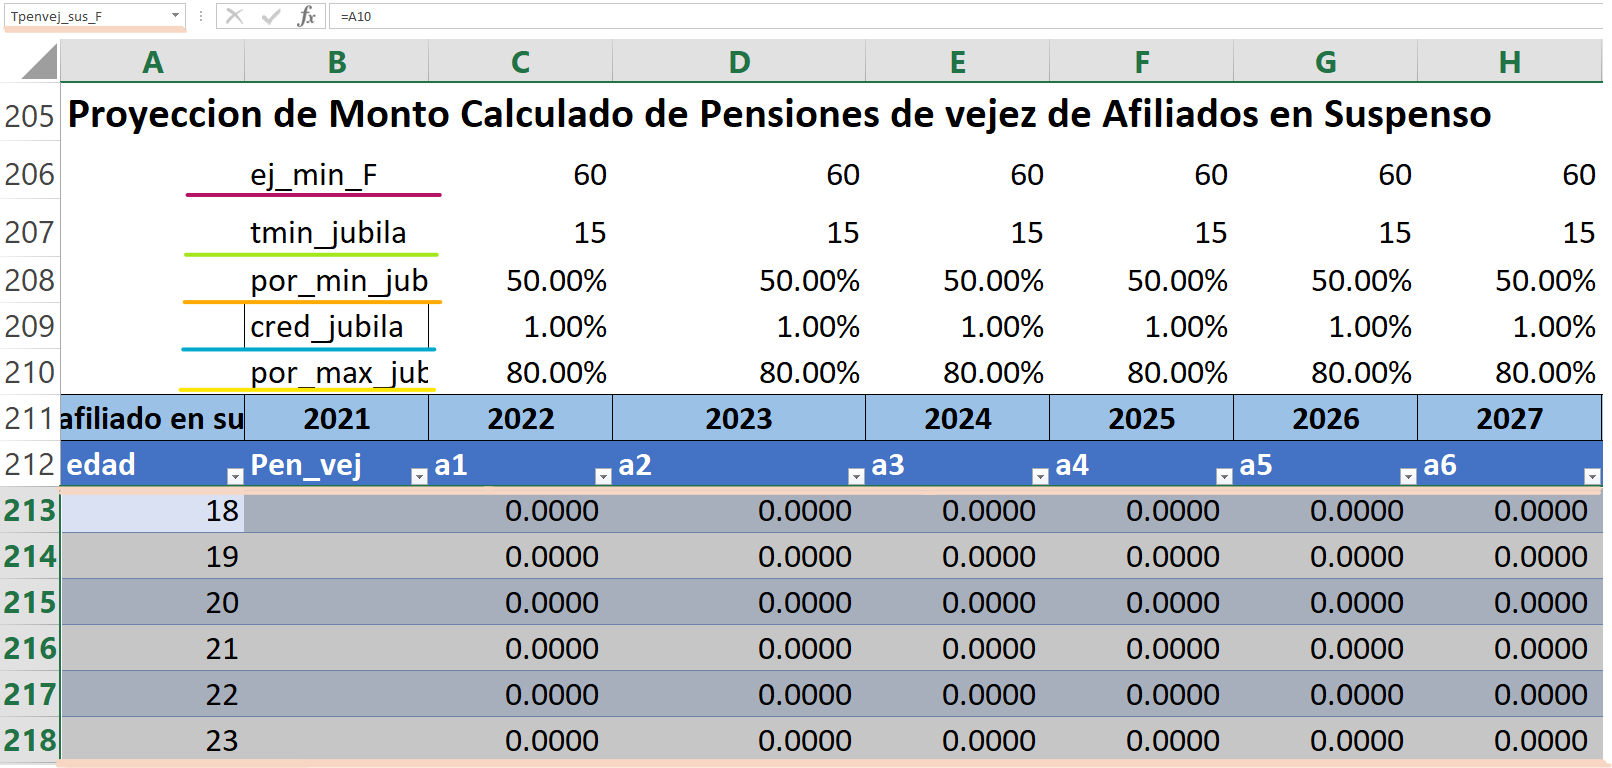
\includegraphics{images/F/Img24.png}

}

\caption{Proyección de pensiones}

\end{figure}

\hypertarget{proyecciuxf3n-de-jubilados}{%
\subsection{Proyección De Jubilados}\label{proyecciuxf3n-de-jubilados}}

Este parámetro representa la cantidad de afiliados en suspenso que se
jubila a lo largo de los años, a dicha tabla se le llamado
\emph{``Tjub\_sus\_M''} para determinar estos valores hacemos uso de la
fórmula 4.3.2 Cantidad de afiliados en suspenso que se jubila que se
encuentra en (Nota Técnica de Proyección de Flujos del Régimen del
Seguro de Previsión Social, a diciembre 2020):

Para dicho cálculo realizamos el producto de \([pja\_dm]\) probabilidad
de jubilarse, \([{CanS}_{x-1,j-1}]\) cantidad de afiliados jubilados en
suspenso del año anterior y edad \emph{x-1} y multiplicado por el factor
\([activar\_susp]\)

\begin{equation}
{jub\_sus}_{j,x}={pja\_dm}_x\times{CanS}_{x-1,j-1}\times activar\_susp
\end{equation}

Donde:

\({CanS}_{x-1,j-1}\) = cantidad de afiliados en suspenso de edad
\emph{x-1} en el año anterior.\\
\(p{ja\_dm}_x\) = probabilidad de decremento múltiple de que un activo
se jubile a la edad \emph{x}.\\
\(activar\_susp\) = factor donde se toma en cuenta la población en
suspenso.

\begin{figure}

{\centering 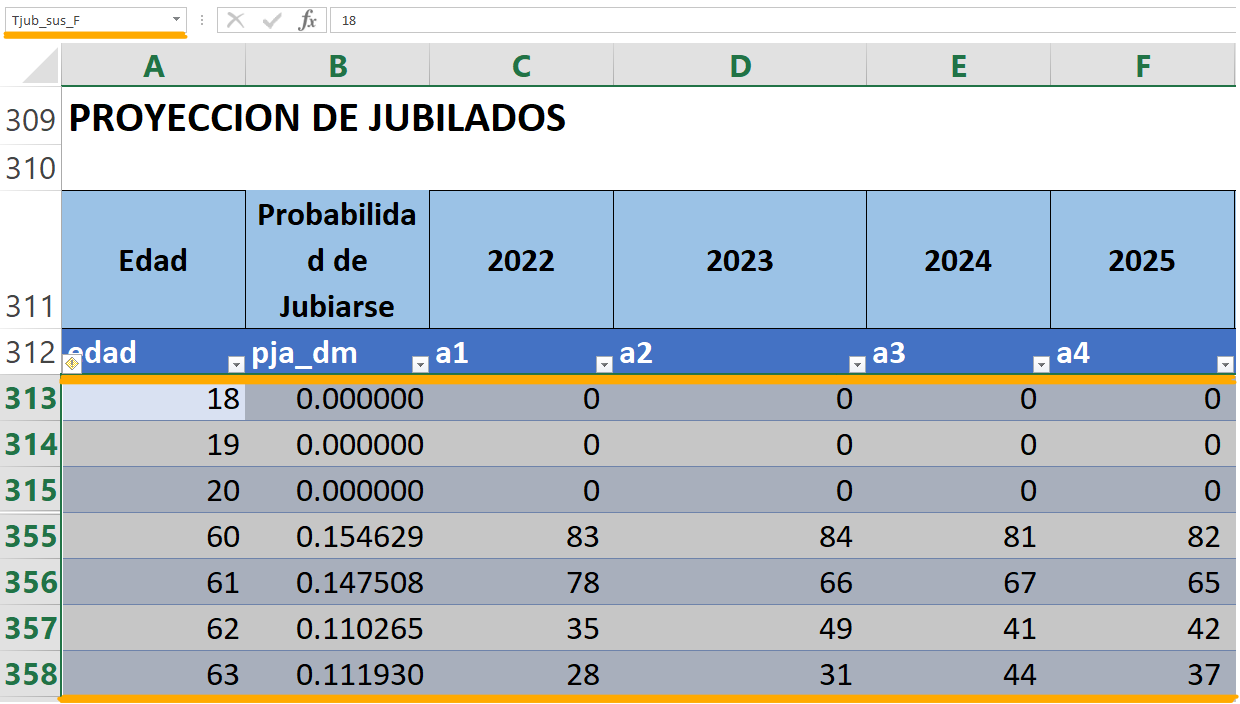
\includegraphics{images/F/Img25.png}

}

\caption{Proyección de jubilados en suspenso}

\end{figure}

\hypertarget{proyecciuxf3n-tiempo-cotizado-de-afiliadas-en-suspenso}{%
\subsection{Proyección Tiempo Cotizado De Afiliadas En
Suspenso}\label{proyecciuxf3n-tiempo-cotizado-de-afiliadas-en-suspenso}}

A esta tabla se le ha llamado \emph{``Ttcot\_sus\_F''} esta contiene el
tiempo promedio de cotización de un afiliado en suspenso por cada edad y
año proyectado.

\begin{equation}
{tcot\_sus}_{x,j}={tcot\_ini}_{x-1,j-1}
\end{equation}

Donde:

\({tcot\_ini}_{x,j}\) = tiempo de cotización inicial de afiliados en
suspenso de edad \emph{x-1} para el año anterior.

\textbf{NOTA}: Todos los parámetros y tablas antes descritas siguen el
mismo patrón y proceso para el caso masculino, habiendo ligeros cambios
en los nombres siendo este cambio por la inicial del género (\emph{M}).

\bookmarksetup{startatroot}

\hypertarget{jubilados}{%
\chapter{Jubilados}\label{jubilados}}

\hypertarget{jubilados-femeninos-jubilados-f}{%
\section{Jubilados Femeninos {[}Jubilados
F{]}}\label{jubilados-femeninos-jubilados-f}}

En esta tabla se encuentra información relevante sobre la cantidad de
Jubilados femeninos que se espera a lo largo de los años proyectados,
también información sobre los salarios, un resumen de todos estos datos
estimados, y otras proyecciones que son importantes para el análisis.

\hypertarget{proyecciuxf3n-de-las-personas-2}{%
\subsection{Proyección de las
personas}\label{proyecciuxf3n-de-las-personas-2}}

A esta tabla en general se le ha llamado \emph{``Tjub\_F''} para
determinar estos datos se toman en cuenta parámetros que se detallan a
continuación:

\begin{itemize}
\tightlist
\item
  {[}\emph{qj}{]} y {[}\emph{pja\_dm}{]} Las probabilidades de fallecer
  y jubilarse respectivamente. Aquí se hace uso de las probabilidades de
  que un afiliado abandone el sistema por vejez, llamados decrementos
  múltiples las cuales se encuentran en la hoja {[}\emph{Tablas}{]} en
  la matriz \emph{``Tbiometrica''}
\item
  {[}\emph{a1-a100}{]} cantidades de afiliados jubilados proyectadas que
  se realizan en el estudio, para este análisis se hace uso de la
  siguiente formula:
\end{itemize}

\begin{align} {CanJ}_{x,j} &= \left(1-{qj}_{x-1}\right)\times{CanJ}_{x-1,j-1} + \nonumber  \\ &\qquad {pja\_dm}_{x-1}\times{Can}_{x-1,j-1\ }+\ {jub\_sus}_{x,j-1} \end{align}

Donde:

\({CanJ}_{x,j}\) = cantidad de afiliados jubilados de edad x* en el año
\emph{j}.\\
\({pja\_dm}_x\) = probabilidad de decremento múltiple de que un activo
se jubile a la edad \emph{x}.\\
\(Can\_{x-1,j-1}\) = cantidad de afiliados activos de edad \emph{x-1} en
el año anterior.\\
\({qj}_x\) = Probabilidad de que un jubilado fallezca a la edad
\emph{x}.\\
\({jub\_sus}_{j,x}\) = cantidad de afiliados en suspenso de edad
\emph{x} en el año \emph{j}, este se encuentra en la tabla
\emph{``Tjub\_sus\_F''} de la hoja Suspenso \emph{F}.

Lo antes descrito es una igualdad a la fórmula 5.3.2 Cantidad de
afiliados jubilados proyectada que se encuentra en (Nota Técnica de
Proyección de Flujos del Régimen del Seguro de Previsión Social, a
diciembre 2020)

\begin{figure}

{\centering 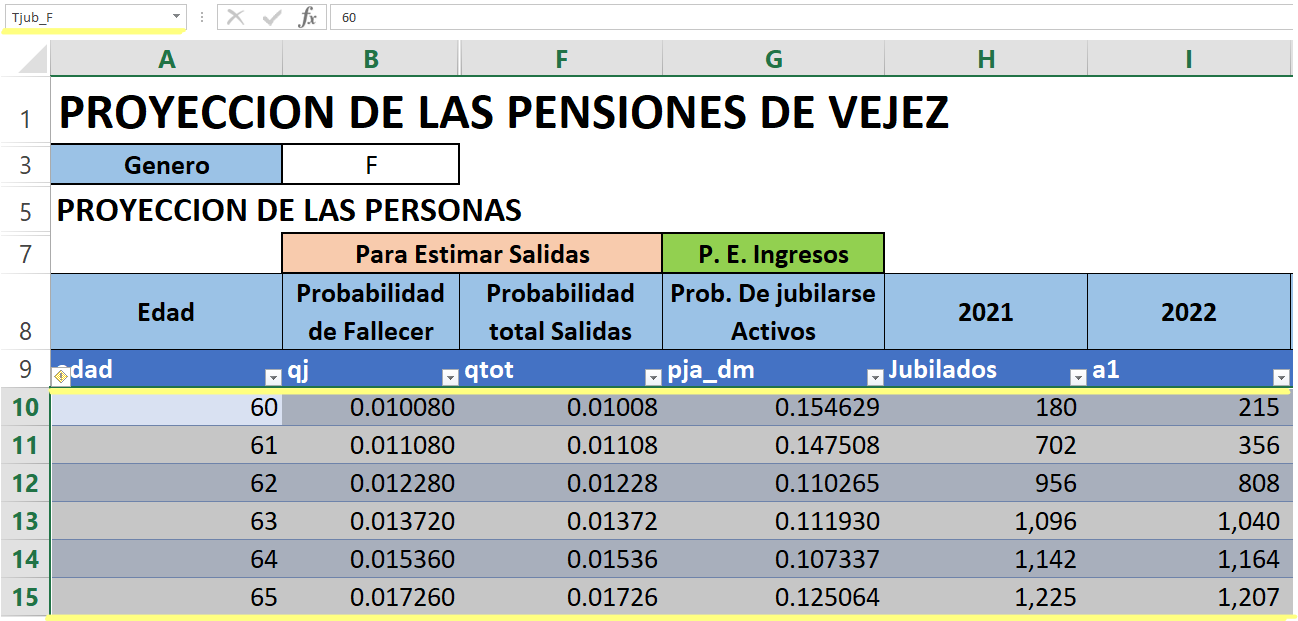
\includegraphics{images/F/Img26.png}

}

\caption{Proyección de jubilados}

\end{figure}

\hypertarget{tabla-resumen-1}{%
\subsection{Tabla Resumen}\label{tabla-resumen-1}}

En esta sección se encuentra un resumen de información relevante entre
ellas, el total de jubilados por años, el porcentaje de crecimiento que
se estima a lo largo de los años entre otras, a continuación se
describen a detalle cada una de estas:

\begin{itemize}
\tightlist
\item
  \([Total]\) esta es la suma de todos los afiliados jubilados
  proyectados por año de todas las edades.
\end{itemize}

\begin{equation}
Total_j=\sum_{x=18}^{110}{C{anJ}_{x,j}}
\end{equation}

\begin{itemize}
\tightlist
\item
  \([Tasa\_de\_crecimiento]\) representa la tasa de crecimiento
  poblacional proyectada relacionada con el año anterior y el presente,
  para ello se hace uso de la siguiente formula
\end{itemize}

\begin{equation}
{tc}_j=\frac{{Total}_j}{{Total}_{j-1}}-1
\end{equation}

\begin{itemize}
\tightlist
\item
  \([Fallecidos]\) esta representa la suma total de la cantidad
  proyectada de fallecidos jubilados llamada \emph{``Tfall\_JF''} y
  ubicada en la misma tabla.
\end{itemize}

\begin{equation}
{Fallecidos}_j=\sum_{x=18}^{110}{MueJ}_{x,j}
\end{equation}

\begin{figure}

{\centering 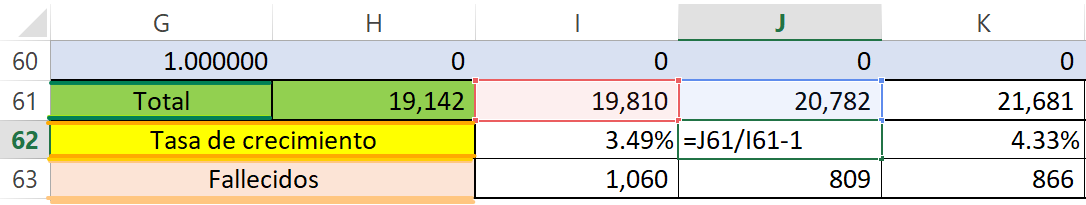
\includegraphics{images/F/Img27.png}

}

\caption{Tabla resumen de jubilados}

\end{figure}

\hypertarget{proyecciuxf3n-de-pensiones}{%
\subsection{Proyección de Pensiones}\label{proyecciuxf3n-de-pensiones}}

Esta tabla llamada \emph{``Tpenjub\_F''} contiene la proyección del
monto por pensiones que se le otorga a un jubilado. Para ello se hace
uso de la siguiente formula, la cual establece una igualdad con la
fórmula 5.3.3 Pensión por vejez que se encuentra en (Nota Técnica de
Proyección de Flujos del Régimen del Seguro de Previsión Social, a
diciembre 2020):

\begin{align}
{Pen\_vJ}_{x,j} & = \nonumber \\ 
& \hspace{2 em}{Pen\_vJ}_{x-1,j-1} \times \left ( 1+trev\_pen_j \right ) \times {CanJ}_{x-1,j-1} \times \left ( 1-{qj}_{x-1} \right ) \nonumber \\
& \underline{ \hspace{1.2 em} +  { Pen\_v}_{x,j}\times{Can}_{x-1,j-1}\times{pja\_{dm}}_{x-1}+{Pen\_vs}_{x,j}\times{jub\_sus}_{x,j} \hspace{2 em}} \nonumber \\
&\hspace{1 em}{CanJ}_{x-1,j-1}\times\left(1-{qj}_{x-1}\right)+{Can}_{x-1,j-1}\times{pja\_{dm}}_{x-1}+{jub\_sus}_{x,j} 
\end{align} Donde:

\({Pen\_vJ}_{x,j}\) = monto calculado de pensión para jubilados de edad
\emph{x} en el año \emph{j}.\\
\({trev\_{pen}}_j\) = tasa de revalorización de pensiones por año
proyectado.\\
\({CanJ}_{x-1,j-1}\) = cantidad de afiliados jubilados de edad
\emph{x-1} en el año anterior.\\
\(Can_{x-1,j-1}\) = cantidad de afiliados activos de edad \emph{x-1} en
el año anterior.\\
\({Pen\_vs}_{x,j}\) = monto calculado de pensión por vejez de afiliados
en suspenso\\
\({Pen\_v}_{x,j}\) = monto calculado de pensión al fallecimiento de
activos, para la base de la pensión por viudez.\\
\({jub\_sus}_{x,j}\) = cantidad de afiliados en suspenso de edad
\emph{x} en el año \emph{j}.

\begin{figure}

{\centering 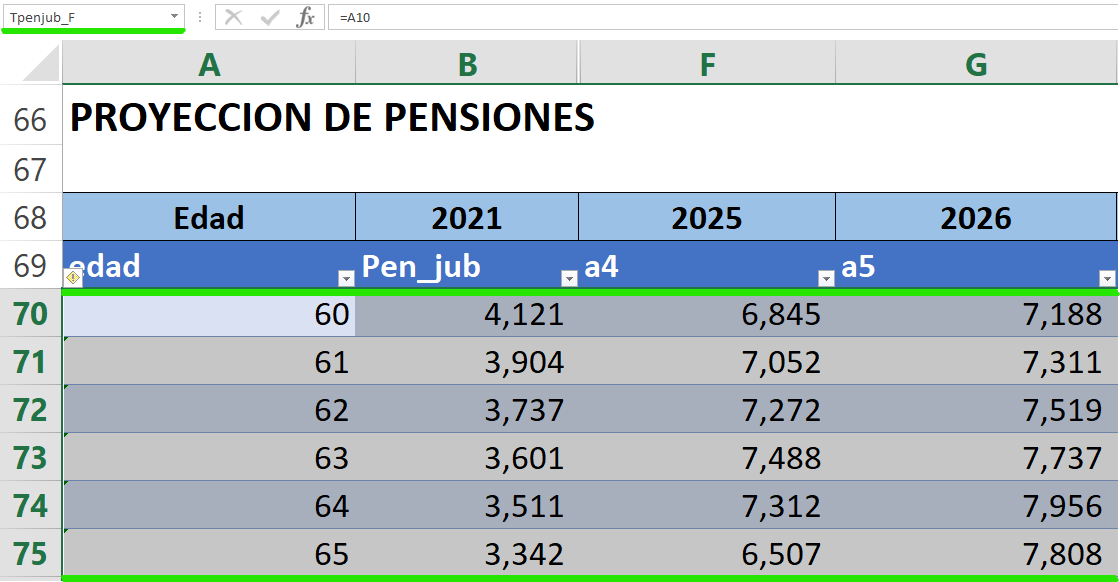
\includegraphics{images/F/Img28.png}

}

\caption{Proyección del Monto calculado de pensión para jubilados}

\end{figure}

\hypertarget{resumen-de-proyecciuxf3n-de-datos-1}{%
\subsection{Resumen de Proyección de
datos}\label{resumen-de-proyecciuxf3n-de-datos-1}}

Aquí se establece un resumen de las contribuciones y ayudas que reciben
los afiliados jubilados de género femenino, a esta tabla se le ha
llamado \emph{``Tresum\_JF''}. Para ello vemos a detalle cada uno de los
parámetros involucrados en dicha tabla

\begin{itemize}
\tightlist
\item
  \([Pensión\ promedio]\) este parámetro contiene el promedio de las
  pensiones para jubilados, para dicho cálculo se hace uso de la fórmula
  5.3.1 Pensión promedio para jubilados que se encuentra en (Nota
  Técnica de Proyección de Flujos del Régimen del Seguro de Previsión
  Social, a diciembre 2020)
\end{itemize}

\begin{equation}
{PensPromJ}_{x,j}= \frac{\sum{CanJ_{x,j}\times Pen{\_vJ}_{x,j}}}{\sum{CanJ_{x,j}}}
\end{equation}

Donde:

\({PensPromJ}_{x,j}\) = pensión promedio para jubilados de edad \emph{x}
en el año \emph{j}.\\
\(CanJ_{x,j}\) = cantidad de afiliados jubilados de edad \emph{x} en el
año \emph{j}.\\
\(Pen{\_vJ}_{x,j}\) = pensión que se le otorga a un jubilado de edad
\emph{x} en el año \emph{j}.

\begin{itemize}
\tightlist
\item
  \([Beneficio\ pensiones]\) este parámetro contiene el total de
  beneficios por pensiones para jubilados, fórmula similar a la fórmula
  5.3.4 Pago total de pensiones por jubilación al año, que se encuentra
  en (Nota Técnica de Proyección de Flujos del Régimen del Seguro de
  Previsión Social, a diciembre 2020)
\end{itemize}

\begin{equation}
{PenJT}_j={num\_pension}_j\times\sum{{Pen\_vJ}_{x,j}\times {CanJ}_{x,j}}
\label{eq:penjt}
\end{equation} Donde:

\(CanJ_{x,j}\) = cantidad de afiliados jubilados a la edad \emph{x} en
el año \emph{j}.\\
\(Pen{\_vJ}_{x,j}\) = pensión que se le otorga a un jubilado a la edad
\emph{x} en el año \emph{j}.\\
\({num\_pension}_j\) = número de pensiones en el año \emph{j}.

\begin{itemize}
\tightlist
\item
  \([Aporte\ de\ salud]\) determina el total de aportes por salud
  proyectada por año y para ello se hace uso de la siguiente formula:
\end{itemize}

\begin{equation}
{Apor\_salud}_j={num\_contri}_j\times{por\_salud}_j\times\ \sum{{Pen\_vJ}_{x,j}\times{CanJ}_{x,j}}
\end{equation}

\begin{itemize}
\tightlist
\item
  \([Ayuda\ Fúnebre]\) este parámetro representa la cantidad que se les
  dará a los familiares de los derecho-habientes jubilados, pensionados
  o fallecidos para gastos fúnebres, aquí se realiza un cálculo total
  por año proyectado, para ello se aplica la siguiente formula:
\end{itemize}

\begin{equation}
AFunebr{eJ}_j=\ AFunbr{eJ}_{j-1}\times(1+{tcrece\_afunebre}_j)
\end{equation}

Donde:

\(AFunbr{eJ}_j\) = ayuda que se otorga en el año \emph{j}.\\
\(AFunbr{eJ}_{j-1}\) = ayuda que se otorga en el año anterior.\\
\(tcrece\_afunebre\) = tasa de incremento del salario de referencia para
otorgar beneficio de ayuda por sepelio.

\begin{itemize}
\tightlist
\item
  \([Tot.\ Ben.\ A.\ F.]\) Total de beneficios por ayuda fúnebre, este
  parámetro representa la cantidad total de beneficios que se conceden
  por ayuda fúnebre por toda la cantidad de fallecidos para el año
  proyectado.
\end{itemize}

\begin{equation}
Tot.Ben.A.f_j = AyudaFunebre_j\times{Fallecidos}_j
\end{equation}

\begin{figure}

{\centering 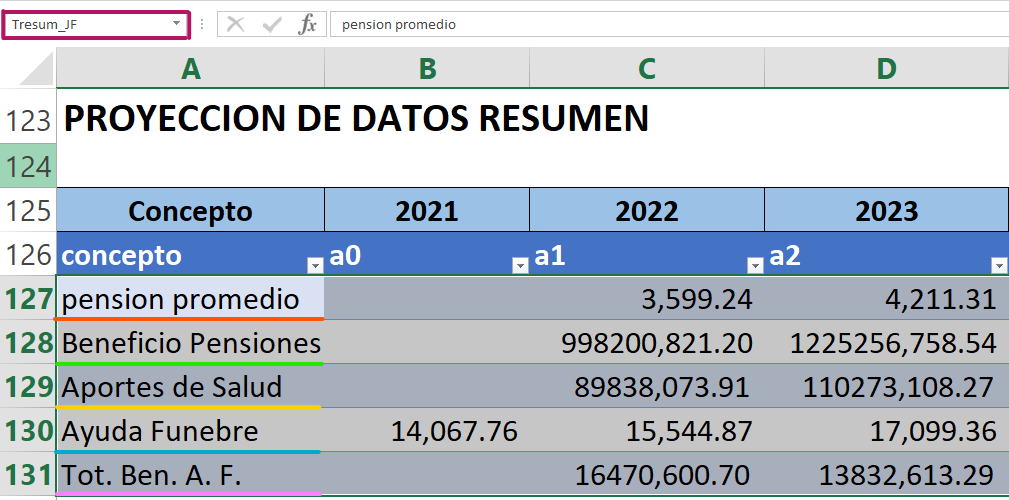
\includegraphics{images/F/Img29.png}

}

\caption{Resumen de datos para Jubilados}

\end{figure}

\hypertarget{proyecciuxf3n-de-viudos-1}{%
\subsection{Proyección de viudos}\label{proyecciuxf3n-de-viudos-1}}

A esta tabla se le llama \emph{``Tnviudez\_JFM''} aquí se estima la
proyección de viudos por la muerte de un jubilado, también se toma en
cuenta la probabilidad de fallecer para una jubilada y la probabilidad
de estar casada,

\begin{equation}
{CanV\_J}_{j,x}={qj}_{x-1}\times pcas_{x-1}\times{CanJ}_{j-1,x-1-5}
\end{equation}

Donde:

\(Can{V\_J}_{j,x}\) = cantidad de viudeces por la muerte de un jubilado
de edad \emph{x} en el año \emph{j}.\\
\({qj}_{x-1}\) = probabilidad de que un jubilado fallezca a la edad
\emph{x-1}.\\
\(pcas_{x-1}\) = probabilidad de que un afiliado este casado a la edad
\emph{x-1}.\\
\({CanJ}_{x-1-5,j-1}\) = cantidad de afiliados jubilados de edad
\emph{x-1} en el año anterior.

\begin{figure}

{\centering 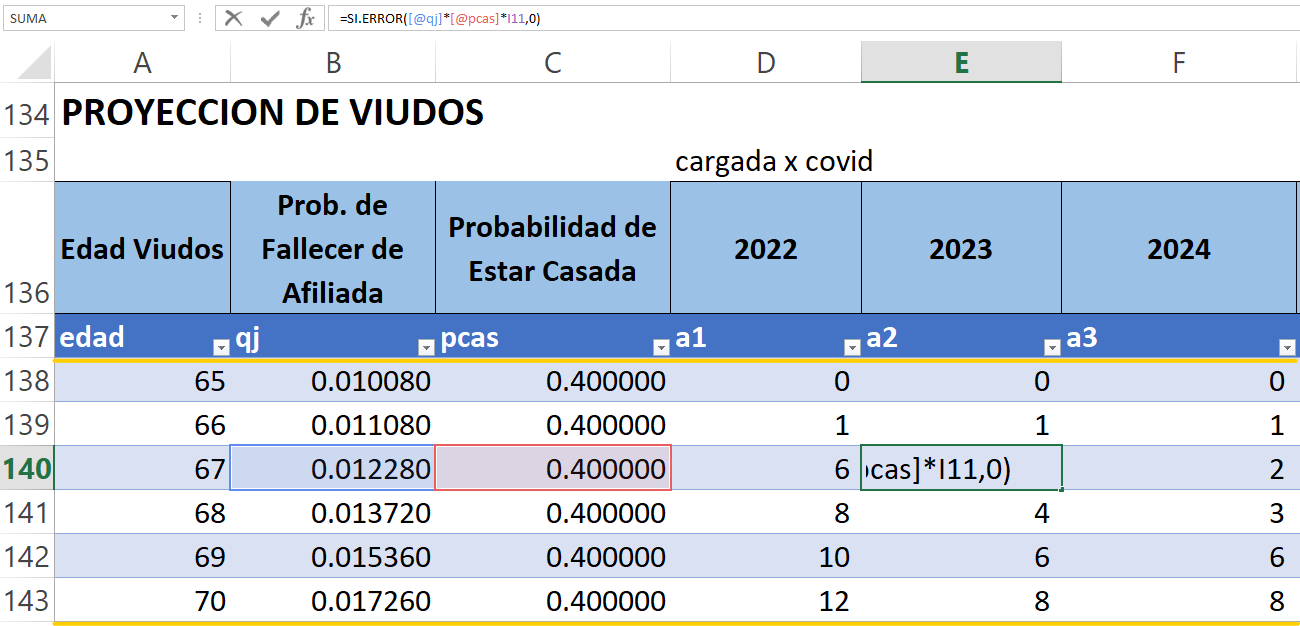
\includegraphics{images/F/Img30.png}

}

\caption{Cantidad de viudos por la muerte de un jubilado}

\end{figure}

\hypertarget{proyecciuxf3n-del-producto-de-monto-pensiuxf3n-por-nuxfamero-de-pensiones-nuevas-de-viudez-para-la-base-de-cuxe1lculo-de-la-pensiuxf3n-promedio-de-viudez}{%
\subsection{Proyección del producto de monto pensión por número de
pensiones nuevas de viudez, para la base de cálculo de la pensión
promedio de
viudez}\label{proyecciuxf3n-del-producto-de-monto-pensiuxf3n-por-nuxfamero-de-pensiones-nuevas-de-viudez-para-la-base-de-cuxe1lculo-de-la-pensiuxf3n-promedio-de-viudez}}

A esta tabla se le ha llamado \emph{``Tnew\_penxnum\_JFM''}, aquí se
determina el monto total para las pensiones por viudeces a la muerte de
un jubilado femenino, estos parámetros son el resultado de la
multiplicación del monto de pensión proyectado para la jubilada ubicados
en la tabla \emph{``Tpenjub\_F''} y el número de viudos proyectados
ubicados en la tabla \emph{``Tnviudez\_JFM''}.

\begin{equation}
{TPen\_vJ}_{x,j}={Pen\_vJ}_{x,j}\times{CanV\_J}_{x,j}
\end{equation}

Donde:

\({TPen\_vJ}_{x,j}\)= Monto Total de pensión al fallecimiento de un
jubilado de edad \emph{x} en el año \emph{j}.\\
\({Pen\_vJ}_{x,j}\)= Monto de pensión al fallecimiento de un jubilado de
edad \emph{x} en el año \emph{j}.\\
\(Can{V\_J}_{x,j}\) = Cantidad de viudos al fallecimiento de un jubilado
de edad \emph{x} en el año \emph{j}.

\begin{figure}

{\centering 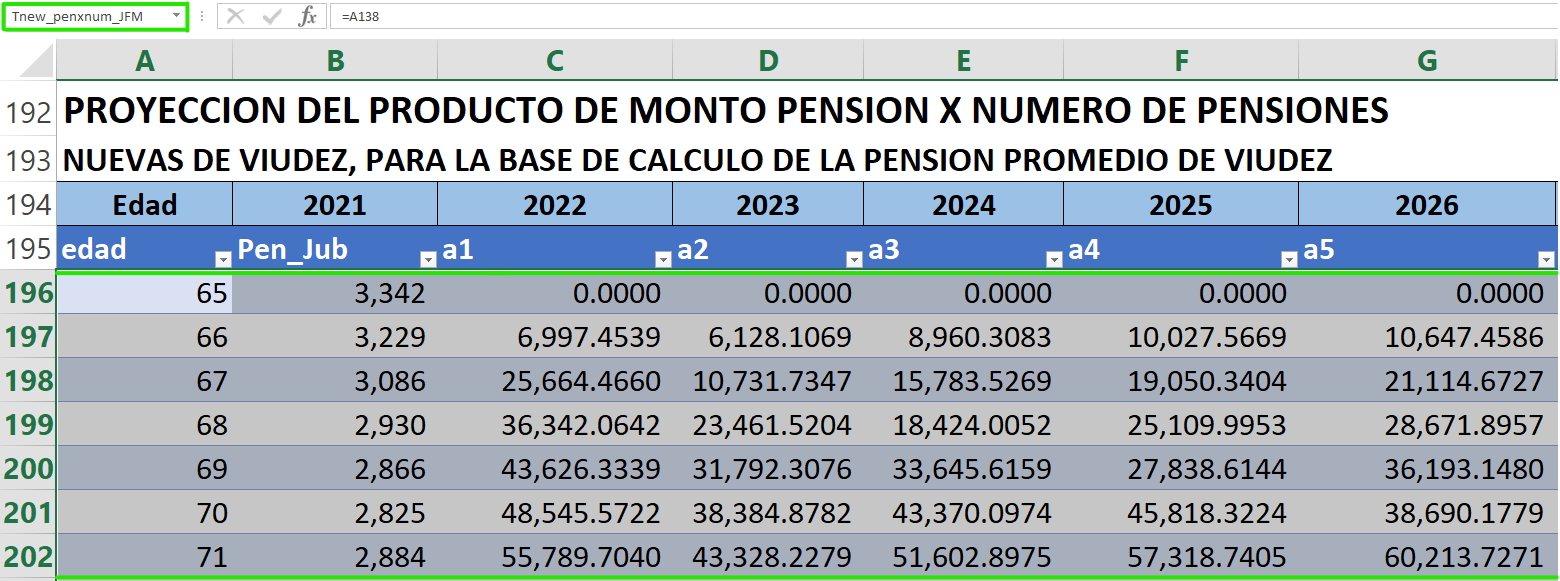
\includegraphics{images/F/Img31.png}

}

\caption{Monto total para las pensiones por viudeces a la muerte de un
jubilado}

\end{figure}

\hypertarget{proyecciuxf3n-fallecidos-activos}{%
\subsection{Proyección fallecidos
activos}\label{proyecciuxf3n-fallecidos-activos}}

a esta tabla se le ha llamado \emph{``Tfall\_JF''}, aquí se establece la
cantidad de jubilados que fallecen, estos parámetros se determinan
haciendo el producto de la probabilidad de fallecer para un jubilado y
la cantidad de personas proyectadas por edad \emph{x} y por año \emph{j}
ubicados en la tabla \emph{``Tjub\_F''}. Para ello se hace uso de la
siguiente formula, la cual establece una igualdad con la fórmula 5.3.5
Cantidad de jubilados que fallecen en (Nota Técnica de Proyección de
Flujos del Régimen del Seguro de Previsión Social, a diciembre 2020):

\begin{equation}
MueJ_{x,j}=CanJ_{x-1,j-1}\times{qj}_{x-1}
\end{equation}

Donde:

\(MueJ_{x,j}\) = cantidad de jubilados que fallecen a la edad \emph{x}
en el año \emph{j}.\\
\(CanJ_{x-1,j-1}\) = cantidad de afiliados jubilados de edad \emph{x-1}
en el año anterior.\\
\({qj}_{x-1}\) = probabilidad de que un jubilado fallezca a la edad
\emph{x-1}.

\begin{figure}

{\centering 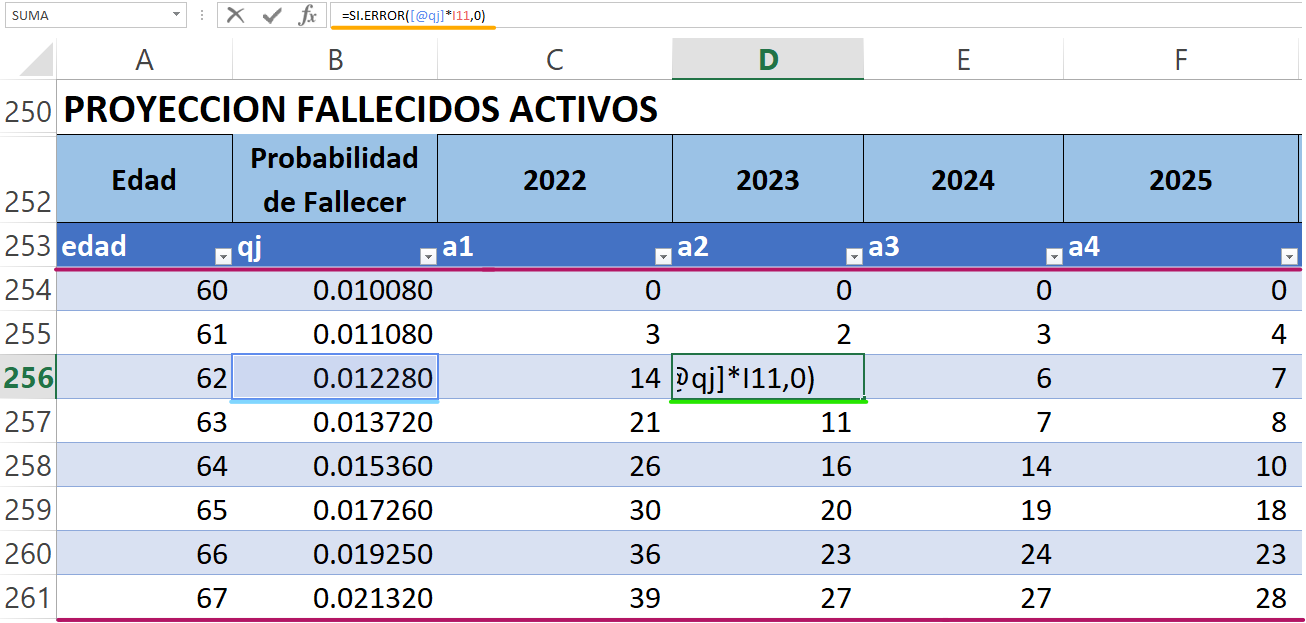
\includegraphics{images/F/Img32.png}

}

\caption{Cantidad de jubilados que fallecen}

\end{figure}

\hypertarget{proyecciuxf3n-de-fallecidos-por-el-monto-de-pensiuxf3n-1}{%
\subsection{Proyección de fallecidos por el monto de
pensión}\label{proyecciuxf3n-de-fallecidos-por-el-monto-de-pensiuxf3n-1}}

A esta tabla se le ha llamado \emph{``Tpenfall\_JF''} Este parámetro
determina la cantidad de pensión proyectada para un jubilado fallecido,
se obtiene multiplicando la probabilidad de fallecer por el monto
calculado de pensiones al fallecimiento de un jubilado en la tabla
\emph{``Tpenjub\_F''} y la cantidad de activos proyectados para el año
anterior ubicado en la tabla \emph{``Tjub\_F''}.

\begin{equation}
{TMueJ}_{x,j}={qj}_{x-1}\times{Pen\_vJ}_{x,j}\times{CanJ}_{x-1+d,j-1}
\end{equation}

Donde:

\({TMueJ}_{j,x}\) = cantidad total montos de pensiones por fallecimiento
de jubilado de edad \emph{x} en el año \emph{j}.\\
\({qj}_{x-1}\) = probabilidad de que un jubilado fallezca a la edad
\emph{x-1}.\\
\(Ca{nJ}_{j-1,x-1+d}\) = cantidad de afiliados jubilados proyectada de
edad de \emph{x-1+d} años para el año anterior, \emph{d = 0} en caso
femenino y \emph{d = 5} en caso masculino.\\
\({Pen\_vJ}_{x,j}\) = monto de pensión al fallecimiento de un jubilado
de edad \emph{x} en el año \emph{j}.

\begin{figure}

{\centering 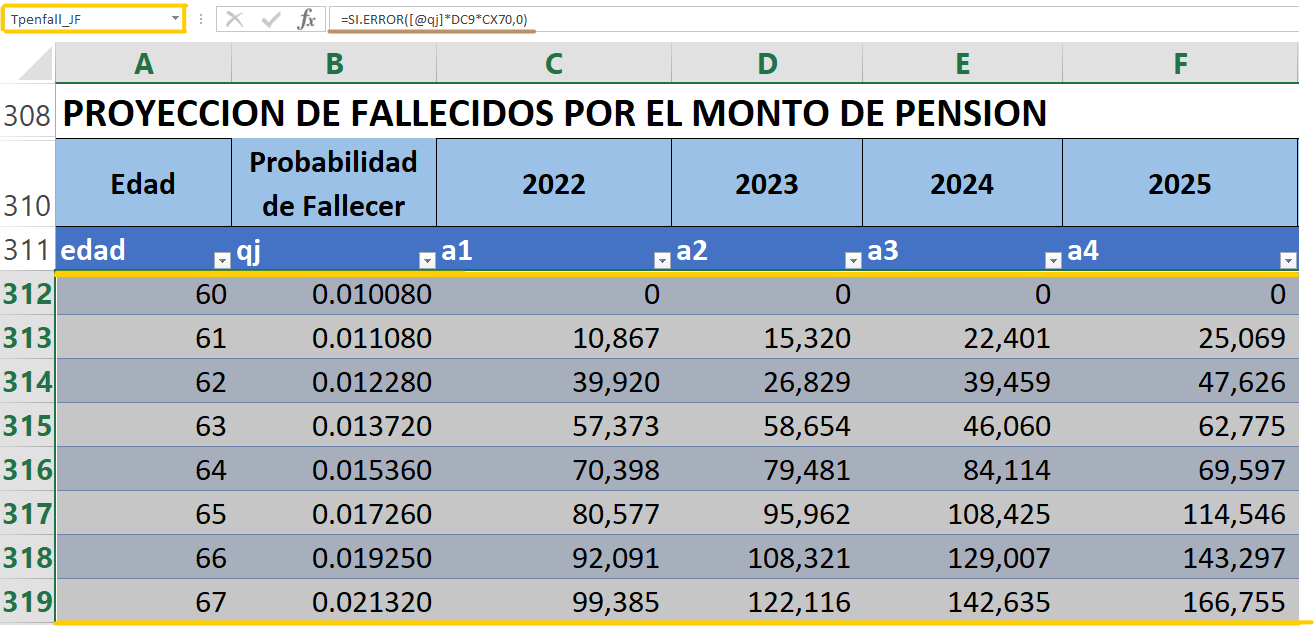
\includegraphics{images/F/Img33.png}

}

\caption{cantidad de pensión proyectada para un jubilado fallecido}

\end{figure}

\textbf{NOTA}: Todos los parámetros y tablas antes descritas siguen el
mismo patrón y proceso para el caso masculino, habiendo ligeros cambios
en los nombres siendo este cambio por la inicial del género (\emph{M}).

\bookmarksetup{startatroot}

\hypertarget{invuxe1lidos}{%
\chapter{Inválidos}\label{invuxe1lidos}}

\hypertarget{invalidez-femenina-invuxe1lidos-f}{%
\section{Invalidez Femenina {[}Inválidos
F{]}}\label{invalidez-femenina-invuxe1lidos-f}}

En esta tabla se encuentra información detallada sobre la cantidad de
inválidos femeninos que se espera a lo largo de los años proyectados,
información sobre los montos por invalidez, un resumen de todos estos
datos estimados, y otras proyecciones que son relevantes para el
análisis, las cuales describimos a continuación:

\hypertarget{proyecciuxf3n-de-las-personas-3}{%
\subsection{Proyección de las
personas}\label{proyecciuxf3n-de-las-personas-3}}

A esta tabla en general se le ha llamado \emph{``Tinv\_F''} aquí se
determinan la cantidad de afiliados en estado de invalidez a lo largo de
los años proyectados, para determinar estos datos se hacen uso de una
serie de parámetros que detallaremos a continuación:

\begin{itemize}
\item
  \([qi]\) y \([ia\_dm]\) estas son las probabilidades de fallecer e
  invalidarse respectivamente. Aquí se hace uso de las Probabilidad de
  que un inválido fallezca a la edad \emph{x} y la Probabilidad de
  decremento múltiple de que un activo se invalide a la edad \emph{x},
  las cuales se encuentran en la hoja \emph{{[}Tablas{]}} en la matriz
  \emph{``Tbiometrica''}.
\item
  \([a1-a100]\) son las cantidades de personas proyectadas que se
  realizan en el estudio, para este análisis se hace uso de la siguiente
  formula:
\end{itemize}

\begin{equation}
{CanI}_{x,j}=\ {Can}_{x-1,j-1}\times{ia\_dm}_{x-1}+{CanI}_{x-1,j-1}\times\left(1-{qi}_{x-1}\right)
\end{equation}

Donde:

\({CanI}_{j,x}\) = cantidad de afiliados en estado de invalidez de edad
\emph{x} en el año \emph{j}.\\
\({Can}_{j-1,x-1}\) = cantidad de afiliados activos de edad \emph{x-1}
en el año anterior.\\
\({CanI}_{j-1,x-1}\) = cantidad de afiliados inválidos de edad
\emph{x-1} en el año anterior.\\
\({ia\_dm}_{x-1}\) = probabilidad de decremento múltiple de que un
activo se invalide a la edad \emph{x-1}.\\
\({qi}_{x-1}\) = probabilidad de que un inválido fallezca a la edad
\emph{x-1}.

Lo antes descrito es una igualdad a la fórmula 6.3.1 y 6.3.2 Cantidad de
afiliados en estado de invalidez por edad y Cantidad de afiliados en
estado de invalidez que fallecen respectivamente y que se encuentra en
(Nota Técnica de Proyección de Flujos del Régimen del Seguro de
Previsión Social, a diciembre 2020):

\begin{figure}

{\centering 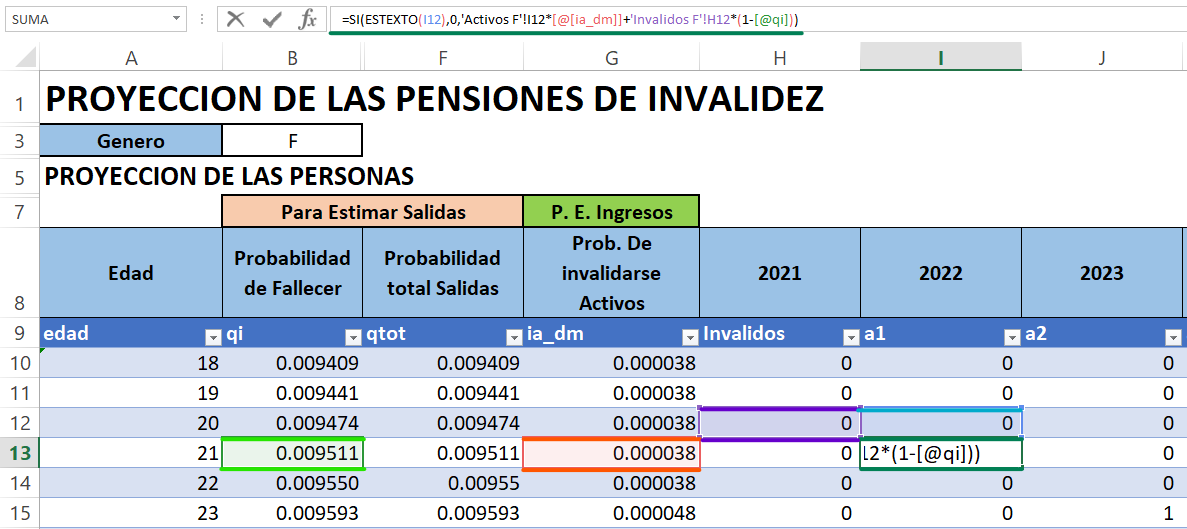
\includegraphics{images/F/Img34.png}

}

\caption{Cantidad de afiliados en estado de invalidez}

\end{figure}

\hypertarget{tabla-resumen-2}{%
\subsection{Tabla Resumen}\label{tabla-resumen-2}}

En esta sección se encuentra un resumen de los datos proyectados para
este estado como ser el total de inválidos por años, el porcentaje de
crecimiento que se estima a lo largo de los años entre otras, a esta
tabla se le ha llamado \emph{``Tresum\_IF''}. a continuación se
describen a detalle cada una de estas:

\begin{itemize}
\tightlist
\item
  \([Total]\) Es la suma de todos los afiliados en estado de invalidez
  proyectados por año.
\end{itemize}

\begin{equation}
Total_j=\sum_{x=18}^{110}{C{anI}_{x,j}}
\end{equation}

Donde:

\(C{anI}_{x,j}\) = cantidad de afiliados en estado de invalidez de edad
\emph{x} en el año \emph{j}.

\begin{itemize}
\tightlist
\item
  \([Tasa\ de\ crecimiento]\) representa la tasa de crecimiento
  poblacional proyectada relacionada con el año anterior y el presente,
  para ello se hace uso de la siguiente formula
\end{itemize}

\begin{equation}
{tc}_j=\frac{{Total}_j}{{Total}_{j-1}}-1
\end{equation}

\begin{itemize}
\tightlist
\item
  \([Fallecidos]\) representa la suma total de la cantidad proyectada de
  fallecidos en estado de invalidez llamada \emph{``Tfall\_IF''} y
  ubicada en la misma tabla. Para ello hacemos uso de lo siguiente
\end{itemize}

\begin{equation}
{Fallecidos}_j=\sum_{x=18}^{110}{MueI}_{x,j}
\end{equation}

\begin{figure}

{\centering 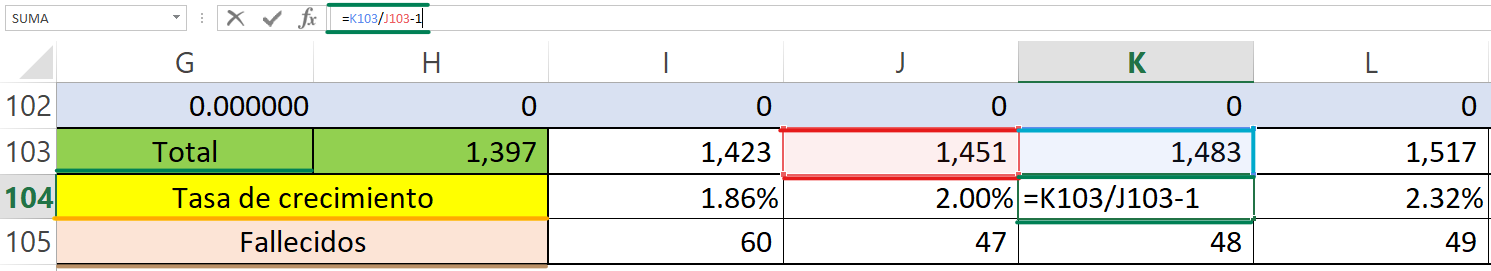
\includegraphics{images/F/Img35.png}

}

\caption{Tabla resumen de afiliados en estado de invalidez}

\end{figure}

\hypertarget{proyecciuxf3n-de-pensiones-1}{%
\subsection{Proyección de
Pensiones}\label{proyecciuxf3n-de-pensiones-1}}

Esta tabla llamada \emph{``Tpeninv\_F''} contiene la proyección del
monto por pensiones que se le otorga a un inválido. Para ello se hace
uso de la siguiente formula, la cual establece una igualdad con la
fórmula 6.3.3 Pensión por invalidez que se encuentra en (Nota Técnica de
Proyección de Flujos del Régimen del Seguro de Previsión Social, a
diciembre 2020)

\begin{align}
Pen\_vI_{x,j} = \nonumber \\
& Pen\_vI_{x-1,j-1} \times \left (1+trevpen_j \right ) \times ia\_dm_{x-1}\times \left(1-qi_{x-1}\right) \nonumber \\
& \underline{\hspace{4 em}+Pen\_v_{x+5,j}\times Can_{x-1,j-1}\times ia\_dm_{x-1} \hspace{4 em}}\nonumber \\ 
&\hspace{1 em} CanI_{x-1,j-1}\times\left(1-qi_{x-1}\right)+Can_{x-1,j-1}\times ia\_dm_{x-1}
\end{align}

Donde:

\({Pen\_vI}_{x,j}\) = monto de pensión al fallecimiento de un inválido
de edad \emph{x} en el año \emph{j}.\\
\({Pen\_vI}_{x-1,j-1}\) = monto de pensión al fallecimiento de un
inválido de edad \emph{x-1} en el año anterior.\\
\({Pen\_v}_{x+5,j}\) = monto de pensión al fallecimiento de un activo de
edad \emph{x} en el año \emph{j}.En este caso como se trata de la tabla
de viudos es necesario igualar esa cantidad de edades, para ello hacemos
uso del factor \emph{x+5}.\\
\({trev\_{pen}}_j\) = tasa de revalorización de pensiones por año
\emph{j} proyectado.\\
\({CanI}_{x-1,j-1}\) = cantidad de afiliados inválidos de edad
\emph{x-1} en el año anterior.\\
\({Can}_{j-1,x-1}\) = cantidad de afiliados activos de edad \emph{x-1}
en el año anterior.\\
\({ia\_dm}_{x-1}\) = probabilidad de decremento múltiple de que un
activo se invalide a la edad \emph{x-1}.\\
\({qi}_{x-1}\) = probabilidad de que un inválido fallezca a la edad
\emph{x-1}.

\textbf{Nota}: Para el caso de análisis comparativo de viudez, para
tener edades comparativas entre estas en caso femenino hay que tener
\emph{x-5} años y para el caso masculino serian \emph{x+5} años.

\begin{figure}

{\centering 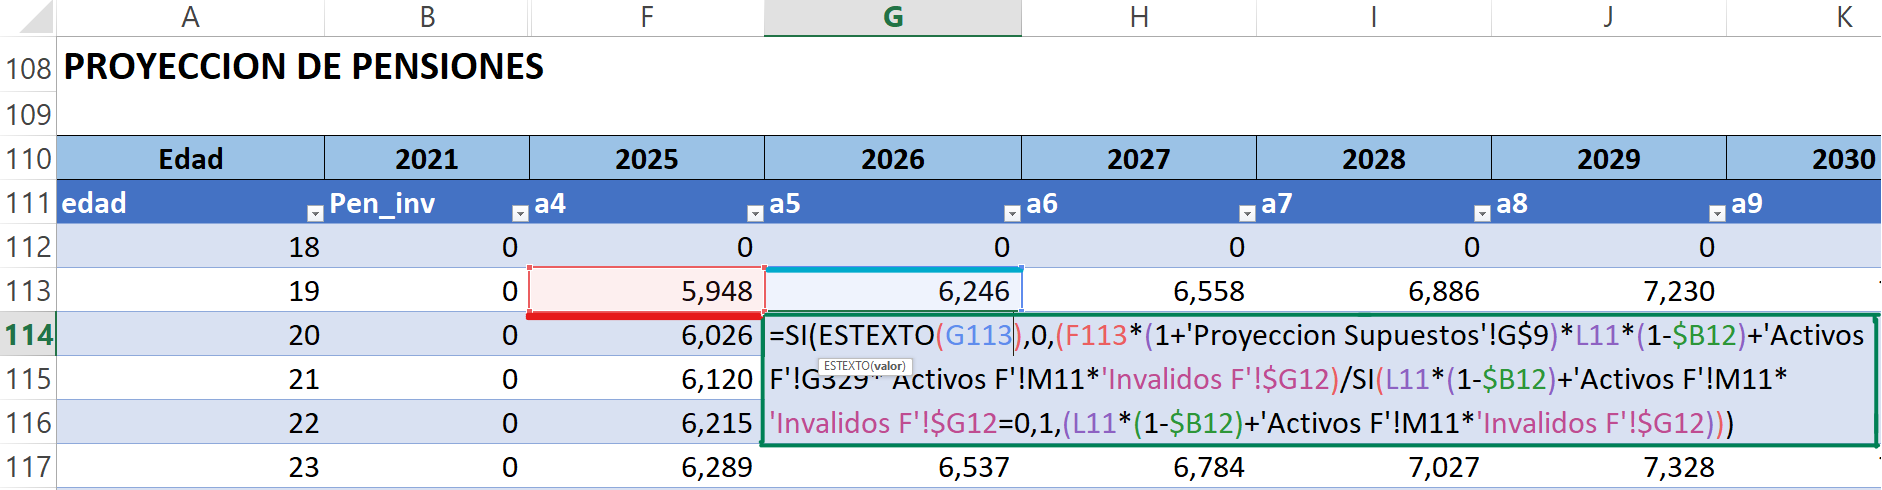
\includegraphics{images/F/Img36.png}

}

\caption{Monto de pensiones que se le otorga a un inválido}

\end{figure}

\hypertarget{resumen-de-proyecciuxf3n-de-datos-2}{%
\subsection{Resumen de Proyección de
datos}\label{resumen-de-proyecciuxf3n-de-datos-2}}

En esta tabla se realiza un resumen de las contribuciones y ayudas que
reciben los afiliados inválidos de género femenino. Para ello vemos a
detalle cada uno de los parámetros involucrados en dicha tabla.

\begin{itemize}
\tightlist
\item
  \([Pensión\ promedio]\) este parámetro contiene el promedio de las
  pensiones para inválidos, para dicho cálculo se hace uso de la fórmula
  6.3.4 Pensión promedio para inválidos que se encuentra en (Nota
  Técnica de Proyección de Flujos del Régimen del Seguro de Previsión
  Social, a diciembre 2020)
\end{itemize}

\begin{equation}
{PensPromI}_{x,j}=\frac{\sum{{Pen\_vI}_{x,j}\times{CanI}_{x,j}}}{Total_j}
\end{equation}

Donde:

\({CanI}_{x,j}\) = cantidad de afiliados inválidos de edad de \emph{x}
en el año \emph{j}.\\
\({Pen\_vI}_{j,x}\) = monto de pensión al fallecimiento de un inválido
de edad \emph{x} en el año \emph{j}.

\begin{itemize}
\tightlist
\item
  \([Beneficio\ pensiones]\) este parámetro contiene el total de
  beneficio por pensiones para invalidez, fórmula similar a la fórmula
  6.3.5 Pago total de pensiones por invalidez al año que se encuentra en
  (Nota Técnica de Proyección de Flujos del Régimen del Seguro de
  Previsión Social, a diciembre 2020)
\end{itemize}

\begin{equation}
{PenIT}_{j}={num\_pension}_j\times\sum{{Pen\_vI}_{x,j}\times{CanI}_{x,j}}
\label{eq:penit}
\end{equation}

Donde:

\({num\_pension}_j\) = número de pensiones en el año \emph{j}.

\begin{itemize}
\tightlist
\item
  \([Aporte\ de\ salud]\) muestra el total de aportes a la salud
  proyectada por año y para ello se hace uso de la siguiente formula
\end{itemize}

\begin{equation}
{Apor\_saludI}_j={num\_contri}_j\times{por\_salud}_j\times\ \sum{{Pen\_vI}_{x,j}\times{CanI}_{x,j}}
\end{equation}

\begin{itemize}
\tightlist
\item
  \([Ayuda\ Fúnebre]\) este parámetro representa la cantidad que se les
  dará a los familiares de los derecho-habientes jubilados, pensionados
  o fallecidos para gastos fúnebres, aquí se realiza un cálculo total
  por año proyectado, para ello se aplica la siguiente formula
\end{itemize}

\begin{equation}
AFunebr{eI}_j=\ AFunbr{eI}_{j-1}\times(1+tcrece\_afunebre)
\end{equation}

Donde:

\(AFunbr{eI}_j\) = ¿ayuda que se otorga en el año \emph{j}.\\
\(AFunbr{eI}_{j-1}\) = ayuda que se otorga en el año anterior.\\
\(tcrece\_afunebre\) = tasa de incremento del salario de referencia para
otorgar beneficio de ayuda por sepelio.

\begin{itemize}
\tightlist
\item
  \([Tot.\ Ben.\ A.\ F.]\) Total de beneficios por ayuda fúnebre, este
  parámetro representa la cantidad total de beneficios que se conceden
  por ayuda fúnebre por toda la cantidad de fallecidos para el año
  proyectado
\end{itemize}

\begin{equation}
Tot.Ben.A.f_j=AyudaFunebre_j\times{Fallecidos}_j
\end{equation}

\begin{figure}

{\centering 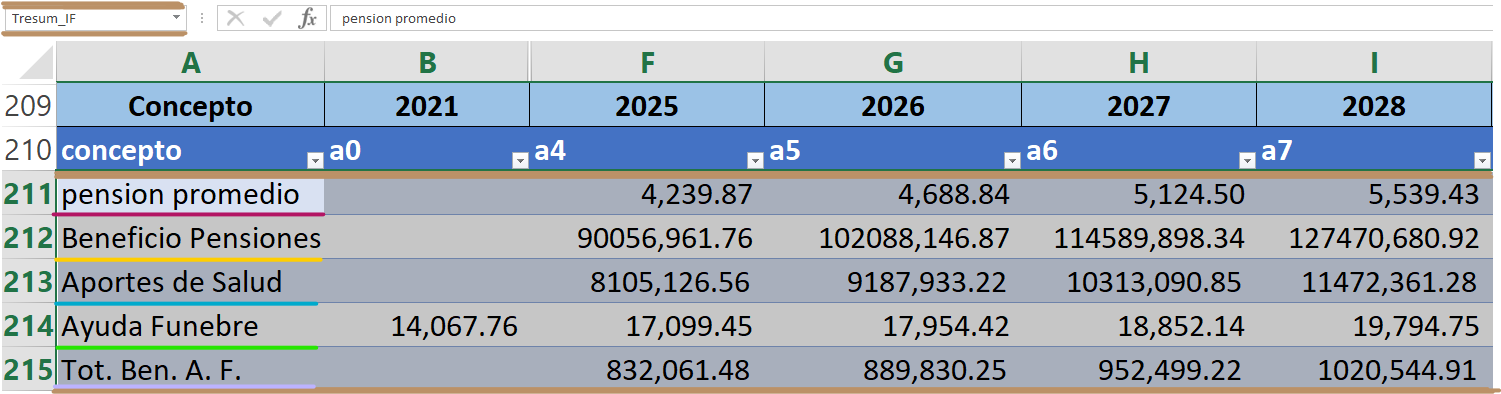
\includegraphics{images/F/Img37.png}

}

\caption{Tabla resumen de proyecciones}

\end{figure}

\hypertarget{proyecciuxf3n-de-viudos-2}{%
\subsection{Proyección de viudos}\label{proyecciuxf3n-de-viudos-2}}

A esta tabla se le llama \emph{``Tnviudez\_IFM''}, aquí se determina el
monto total para las pensiones por viudeces a la muerte de un invalido
femenino, en este caso se realiza una adaptación comparativa en las
edades, recordando que se considera que la edad de jubilación del hombre
es 5 años más, es por eso que se establece la edad \emph{x+5} es esta
tabla. Para estimar la proyección de viudos se toma en cuenta la
probabilidad de fallecer para una inválida y la probabilidad de estar
casada,

\begin{equation}
Can{V\_I}_{x,j}={qi}_{x-1}\times pcas_{x-1}\times{CanI}_{j-1,x-6}
\end{equation}

Donde:

\(Can{V\_I}_{x,j}\) = cantidad de viudos al fallecimiento de un inválido
de edad \emph{x} en el año \emph{j}.\\
\({qi}_{x-1}\) = probabilidad de fallecer de una invalida de edad
\emph{x-1}.\\
\(pcas\_{x-1}\) = probabilidad de que un afiliado este casado a la edad
\emph{x-1}.\\
\({CanI}_{x-1-5,j-1}\) = cantidad de afiliados inválidos proyectados
para el año anterior a la edad \emph{x-6}.

\begin{figure}

{\centering 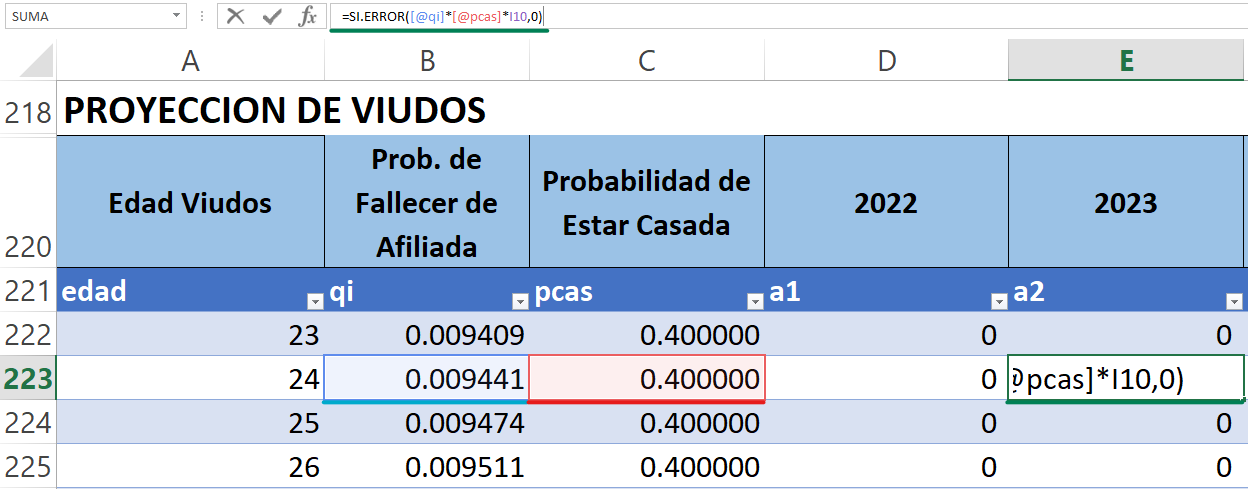
\includegraphics{images/F/Img38.png}

}

\caption{Cantidad de viudos al fallecimiento de un invalido}

\end{figure}

\hypertarget{proyecciuxf3n-del-producto-de-monto-pensiuxf3n-por-nuxfamero-de-pensiones-nuevas-de-viudez-para-calcular-pensiones-promedio-de-invalidez.}{%
\subsection{Proyección del producto de monto pensión por número de
pensiones nuevas de viudez, para calcular pensiones promedio de
invalidez.}\label{proyecciuxf3n-del-producto-de-monto-pensiuxf3n-por-nuxfamero-de-pensiones-nuevas-de-viudez-para-calcular-pensiones-promedio-de-invalidez.}}

A esta tabla se le ha llamado \emph{``Tnew\_penxnum\_IFM''}, y contiene
el monto total de las pensiones que se otorgan por el fallecimiento de
un invalido de edad \emph{x} en el año \emph{j}, estos parámetros son el
resultado de la multiplicación del monto de pensión para edad \emph{x-5}
(se parte de la edad del esposo) y por año proyectado \emph{j} ubicados
en la tabla \emph{``Tpeninv\_F''} y el número de viudos proyectados
\(CanI_{x,j}\) por edad \emph{x} en el año \emph{j} ubicados en la tabla
\emph{``Tnviudez\_IFM''}.

\begin{equation}
{TPen\_vI}_{x,j}={Pen\_vI}_{x,j}\times{CanV\_I}_{x,j}
\end{equation}

Donde:

\({TPen\_vI}_{x,j}\) = monto Total de pensión al fallecimiento de un
inválido de edad \emph{x} en el año \emph{j}.\\
\({Pen\_vI}_{x,j}\) = monto de pensión al fallecimiento de un inválido
de edad x en el año \emph{j}.\\
\(Can{V\_I}_{x,j}\) = cantidad de viudos al fallecimiento de un inválido
de edad \emph{x} en el año \emph{j}.

\begin{figure}

{\centering 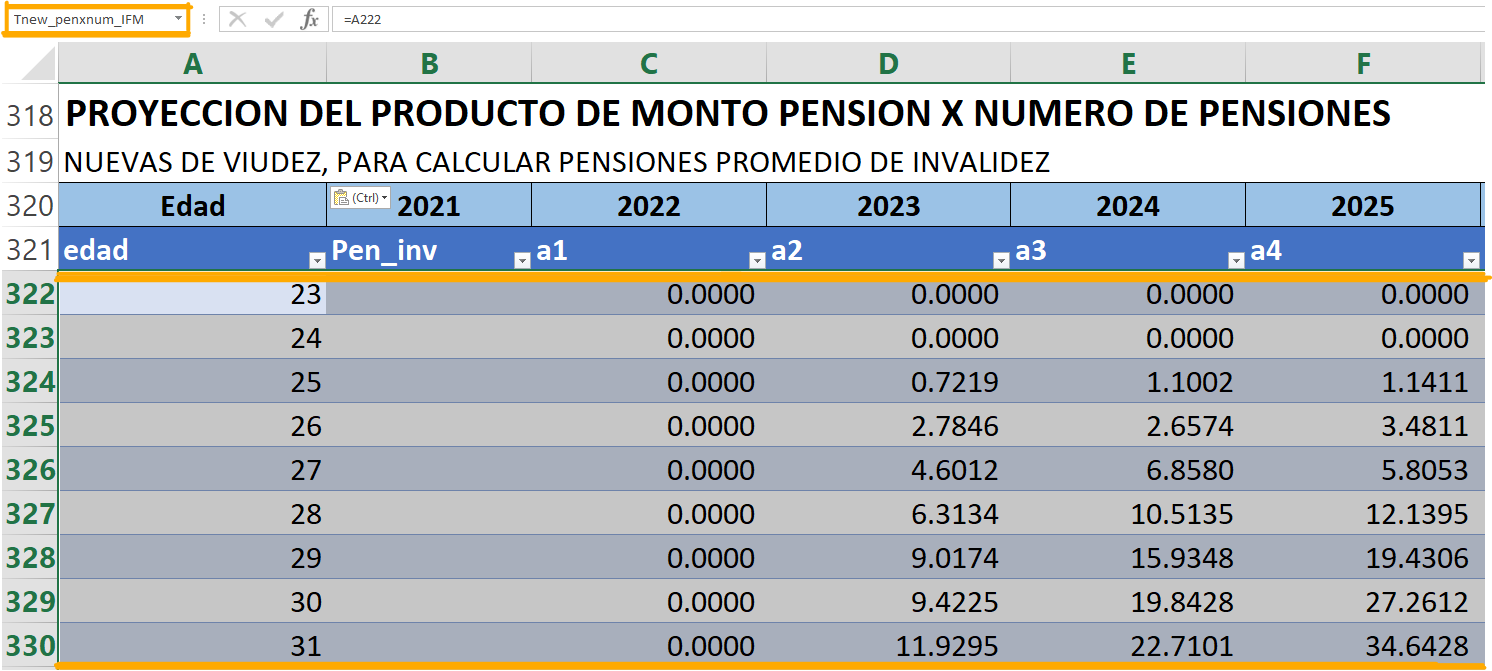
\includegraphics{images/F/Img39.png}

}

\caption{monto total de las pensiones que se otorgan por el
fallecimiento de un invalido}

\end{figure}

\hypertarget{proyecciuxf3n-fallecidos-activos-1}{%
\subsection{Proyección Fallecidos
Activos}\label{proyecciuxf3n-fallecidos-activos-1}}

A esta tabla se le ha llamado \emph{``Tfall\_IF''}, estos parámetros se
determinan haciendo el producto de la probabilidad de fallecer para un
invalido y la cantidad de afiliados en estado de invalidez por edad y
por año proyectado ubicados en la tabla \emph{``Tinv\_F''}. Para ello se
hace uso de la siguiente formula, la cual establece una igualdad con la
fórmula 6.3.2 Cantidad de afiliados en estado de invalidez que fallecen
(Nota Técnica de Proyección de Flujos del Régimen del Seguro de
Previsión Social, a diciembre 2020)

\begin{equation}
MueI_{x,j}=CanI_{x-1,j-1}\times{qi}_{x-1}
\end{equation}

Donde:

\(MueI_{x,j}\) = cantidad de inválidos que fallecen a la edad \emph{x}
en el año \emph{j}.\\
\(CanI_{x-1,j-1}\) = cantidad de afiliados inválidos de edad \emph{x-1}
en el año anterior.\\
\({qi}_{x-1}\) = probabilidad de que un inválido fallezca a la edad
\emph{x-1}.

\begin{figure}

{\centering 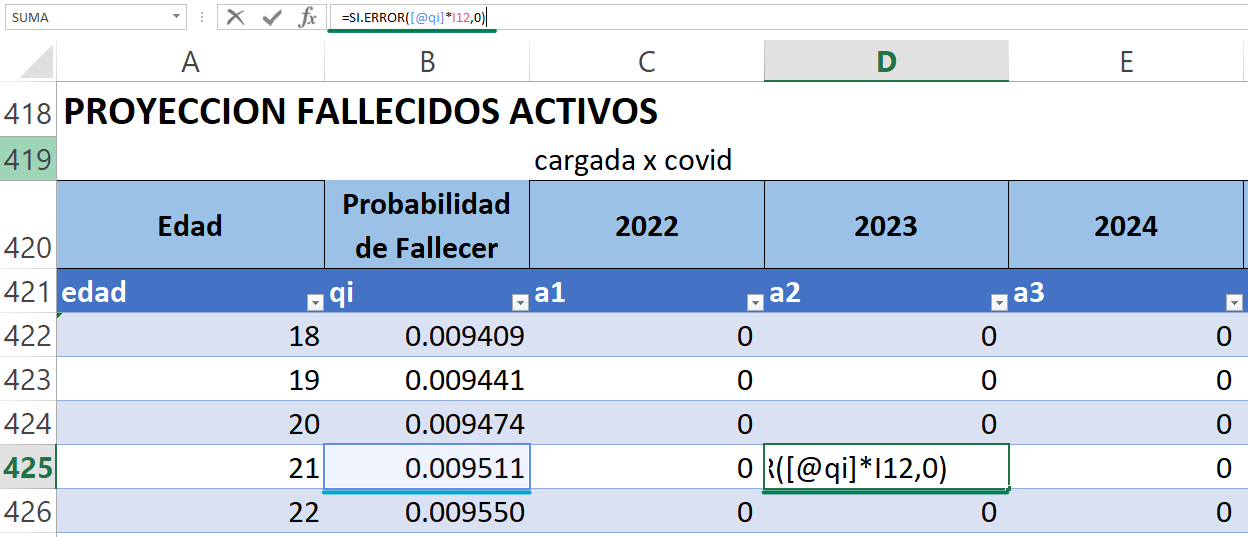
\includegraphics{images/F/Img40.png}

}

\caption{Cantidad de afiliados en estado de invalidez que fallecen}

\end{figure}

\hypertarget{proyecciuxf3n-de-fallecidos-por-el-monto-de-pensiuxf3n-2}{%
\subsection{Proyección De Fallecidos Por El Monto De
Pensión}\label{proyecciuxf3n-de-fallecidos-por-el-monto-de-pensiuxf3n-2}}

A esta tabla se le ha llamado \emph{``Tpenfall\_IF''} Este parámetro
determina la cantidad de pensión proyectada para un invalido que
fallece, se obtiene multiplicando la probabilidad de fallecer para un
invalido por el monto calculado de pensiones al fallecimiento de un
invalido ubicados en la tabla \emph{``Tpeninv\_F''} y la cantidad de
activos proyectados para el año anterior ubicado en la tabla
\emph{``Tinv\_F''}.

\begin{equation}
{TMueI}_{x,j}={qi}_{x-1}\times{Pen\_vI}_{x,j}\times{CanI}_{x-1+d,j-1}
\end{equation}

Donde:

\({TMueI}_{j,x}\) = cantidad total de pensiones por fallecimiento de
inválido de edad \emph{x} en el año \emph{j}.\\
\({qi}_{x-1}\) = probabilidad de que un inválido fallezca a la edad
\emph{x-1}.\\
\(Ca{nI}_{j-1,x-1+d}\) = cantidad de afiliados inválidos proyectada de
edad de \emph{x-1+d} años para el año anterior, \emph{d = 0} en caso
femenino y \emph{d = 5} en caso masculino.\\
\({Pen\_vI}_{x,j}\) = monto de pensión al fallecimiento de un inválido
de edad \emph{x} en el año \emph{j}.

\begin{figure}

{\centering 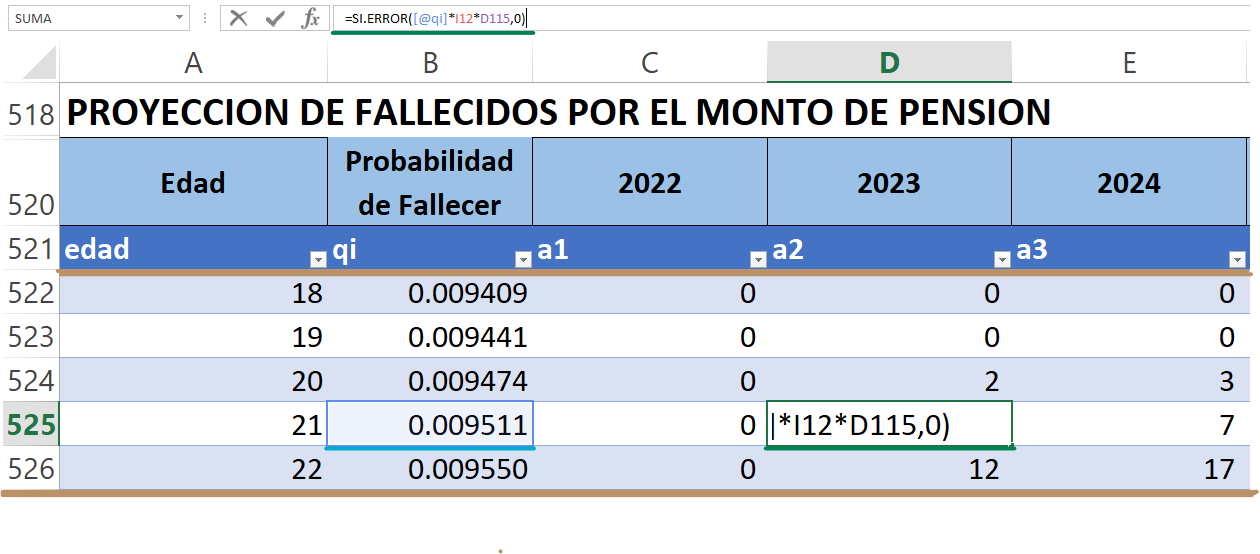
\includegraphics{images/F/Img41.png}

}

\caption{cantidad de pensión proyectada para un invalido que fallece}

\end{figure}

\textbf{NOTA}: Todos los parámetros y tablas antes descritas siguen el
mismo patrón y proceso para el caso masculino, habiendo ligeros cambios
en los nombres siendo este cambio por la inicial del género (\emph{M}).

\bookmarksetup{startatroot}

\hypertarget{references}{%
\chapter*{References}\label{references}}
\addcontentsline{toc}{chapter}{References}

\markboth{References}{References}

\hypertarget{refs}{}
\begin{CSLReferences}{0}{0}
\end{CSLReferences}



\end{document}
